% temp headsep for storage to reset at end of file
\newlength{\headseptemp}
\setlength{\headseptemp}{\headsep}
\setlength{\headsep}{.5cm}
\addtolength{\textheight}{-\headsep}

\DeclareDelimFormat[parencite]{finalnamedelim}{\addspace\&\space}
\DeclareDelimFormat[textcite]{finalnamedelim}{\addspace\&\space}
\DeclareDelimFormat[cite]{finalnamedelim}{\addspace\&\space}

\graphicspath{ {images/} }

\thispagestyle{empty}
\pagenumbering{roman}

{\center
\hfill
\vspace{2cm}

\textbf{\Large
N\textipa{\textvertline}uuki Namagowab Afrikaans English:\\
\textipa{\textdoublebarpipe}Xoaki\textipa{\textdoublebarpipe}xanisi/M\^{\i}di di \textipa{\textdoublebarpipe}Khanis/Woordeboek/Dictionary
}

\vspace{3cm}

\textbf{Chief editors}\\
Bonny Sands, Kerry Jones\\[2em]

\textbf{Editorial team}\\
Chris Collins, Alena Witzlack-Makarevich, Sylvanus Job, Francoise
(Betta) Steyn,\\
Dietloff van der Berg, Dotty Mantzel, Willem Damarah\\[2em]

\textbf{Computational linguist}\\
Menno van Zaanen\\[2em]

\textbf{Additional authors/contributors}\\[1em]

\textbf{Linguists}\\
Amanda Miller, Levi Namaseb, Johanna Brugman, Mats
Exter\\[2em]

\textbf{N\textipa{\textvertline}uu language}\\
Anna (Antjie) Kassie,
Griet Seekoei, Katrina Esau, Hannie Koerant, Andries Olyn,\\
Hanna Koper, Vytjie \textipa{\textvertline}Abaka Koper, Simon Sauls,
\textipa{\textvertline}Una Rooi, Kheis Brou, Elsie Vaalbooi\\[2em]

\textbf{N\textipa{\textvertline}uu Language Authority}\\
Katrina Esau,
Claudia Snyman, David van Wyk, Mietjie Sussie Bok\\[2em]

\textbf{Nama language}\\
Willem Damarah, Lys (Oulet) Kruiper Pietersen,
Izak Kruiper,\\
Lydia (Sakkas) Kruiper, Leonard Gewersk\\[2em]

\textbf{Afrikaans language}\\
Fritz Jagers, Magdalena James, Hannetjie
van der Westhuizen\\[2em]

} % end center

\newpage

%%%%%%%%%%%%%%%%%%%%%%%%%%%%%%%%%%%%%%%%%%%%%%%%%%%%%%%%%%%%%%%%%%%%%%%%%%%%%%%%
\thispagestyle{empty}

\hfill
\vfill

N\textipa{\textvertline}uuki Namagowab Afrikaans English:
\textipa{\textdoublebarpipe}Xoaki\textipa{\textdoublebarpipe}xanisi/M\^{\i}di
di \textipa{\textdoublebarpipe}Khanis/Woordeboek/Dictionary\\[1em]


All rights reserved\\[1em]


Copyright \copyright{} 2022 Bonny Sands and Kerry Jones\\[1em]


The chief editors Bonny Sands and Kerry Jones have made every effort
to obtain permission for and acknowledge the use of copyrighted
material. Refer all enquiries to the chief editors.\\[1em]


No part of this book may be reproduced or transmitted in any form or
by any electronic, photographic or mechanical means, including
photocopying and recording on record, tape or laser disk, on
microfilm, via the Internet, by email, or by any other information
storage and retrieval system, without prior written permission by the
publisher.\\[1em]

Views reflected in this publication are not necessarily those of the
publisher.\\[1em]

The terminology list was authenticated by the Khoi \& San National
Language Body, an advisory and quality assurance structure of PanSALB.
Claudia Snyman, Sussie Bok, working with Ouma Katrina Esau, were
involved in the process of authentication.\\[1em]

First edition 2022\\[1em]

ISBN 978-0-6397-1245-1 (print)\\
ISBN 978-0-6397-1246-8 (e-book)\\[1em]

Set in Computer Modern (10pt)\\[1em]

Project managed by African Tongue\\
\url{https://www.africantongue.co.za}\\
\url{africantongue@gmail.com}\\[1em]

Production by African Sun Media\\[1em]

Cover design: \copyright{} Francoise (Betta) Steyn,
\url{https://www.gimbalmedia.co.za}\hspace{2cm}
\raisebox{-1em}[0pt][0pt]{
\includegraphics[width=4cm]{gimbal.png}}
\\[1em]

Cover photo credit: \textipa{\textdoublebarpipe}Khomani San $|$ Hugh
Brody collection (BVF41), Special Collections, University of Cape Town
Libraries, used with permission from Hugh Brody.

\newpage
%%%%%%%%%%%%%%%%%%%%%%%%%%%%%%%%%%%%%%%%%%%%%%%%%%%%%%%%%%%%%%%%%%%%%%%%%%%%%%%%
\thispagestyle{empty}

\renewcommand{\contentsname}{Inhoud/Contents}
\markboth{}{}
\tableofcontents
\markboth{}{}

\newpage

%%%%%%%%%%%%%%%%%%%%%%%%%%%%%%%%%%%%%%%%%%%%%%%%%%%%%%%%%%%%%%%%%%%%%%%%%%%%%%%%
\thispagestyle{empty}


\markboth{}{}
\section*{Acknowledgements}
\markboth{}{}

We offer our deepest gratitude to the Department of Sport, Arts and
Culture (DSAC) of the Republic of South Africa, for their financial
support of this work \emph{Digital Dictionary Resources for
N\textipa{\textvertline}uu} as a response to the call for \emph{Human
Language Technology Projects}.  Additionally, the South African Centre
for Digital Language Resources (SADiLaR) provided outstanding
computational support crucial in bringing this project to completion.
We are grateful to African Tongue consultancy for administering the
DSAC grant and overseeing the project to a successful conclusion,
especially during difficult pandemic times in our global history.\\

Bonny Sands, Chris Collins, Amanda Miller and Johanna Brugman also
wish to thank the National Science Foundation of the United States for
their support of the research that enabled the creation of this
dictionary. This material is based on work supported by the National
Science Foundation, \emph{Documenting Endangered Languages Program}
under grant \emph{Collaborative Research: Descriptive and Theoretical
Studies of N\textipa{\textvertline}uu} to Cornell University
(BCS-0236735, Miller and Collins, co-PIs) and Northern Arizona
University (BCS-0236795, Sands, PI). Any opinions, findings, and
conclusions or recommendations expressed in this material are those of
the authors and do not necessarily reflect the views of the National
Science Foundation.\\

Alena Witzlack-Makarevich wishes to thank the Endangered Languages
Documentation Programme (ELDP) for their support under the grant
titled \emph{A text documentation of N\textipa{\textvertline}uu} to Max
Planck Institute for Evolutionary \mbox{Anthropology}, Leipzig, Germany
(MDP0157, PI Tom G\"{u}ldemann). We also thank collaborators Tom
G\"{u}ldemann, Sven Siegmund and Martina Ernszt-Shaw for all their
work in creating the corpus sponsored by this grant.\\

Mats Exter would like to thank the University of Cologne and the
German Academic Exchange Service (DAAD) for their support of his
fieldwork.\\

We also wish to thank the South African San Institute (SASI) and Grace
Humphries for facilitating our work and fieldwork translators:
Gertruida Sauls, Collin Louw, Magdalena Kassie, Karen Basson, Willem
Damarah and Gerhardus Damarah. We also thank Men\'{a}n Du Plessis for
extensive comments on an early version of the dictionary and for her
encouragement to apply for funding enabling us to significantly
enhance the quality of the work by including South African Nama and
local Afrikaans translations.\\

\begin{tabular}{lcc}
    
\includegraphics[width=6.3cm]{dsac.jpg} &
    
\includegraphics[width=5cm]{at.jpg} &
    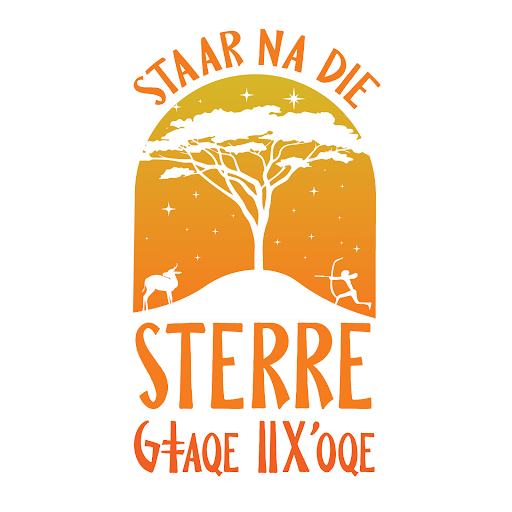
\includegraphics[width=3cm]{sterre.png} \\
    
\includegraphics[width=6cm]{dsi.png} &
    
\includegraphics[width=5cm]{sadilar.png} &
    
\includegraphics[width=5cm]{sun.jpg} \\
\end{tabular}

\newpage

\pagenumbering{arabic}


\section*{Elsie !Uxe Vaalbooi, 1997 -- Metafoor vir die herontmoeting met
N\textipa{\textvertline}uu\ldots}

``Praat ons, ons taal. Ek s\^{e}, hier is die man wat ek gekry het --
die eerste man -- en hy het weggeraak\ldots{} Laat ek hom nou nie sien.
Nou weet hy nie wat soek ek nie\ldots{} ek kon amper nie met hom praat
nie. Maar ek moet met hom praat, want hy't moeite gedoen om te kom. En
ek is bly om hom te sien en te groet. Maar nou praat ek nie meer nie,
ek loop l\^{e}, ek is siek. En met ons alles, my mense, ek dink ek het
seker nou genoeg gepraat. En waar ek sal nog 'n bietjie praat waar ons
alleen is sodat ek kan asem kry. Ek meen dat hy (Nigel Crawhall) vir
my vra dat ek byval wat ek ges\^{e} het om voor te loop nog s\^{e}. Ek
dink ek het nog 'n bietjie om te s\^{e}. Maar ek sal nou op hierdie
huidige oomblik, sal ek dit nie s\^{e} nie, want ek is moeg. Ek het my
nou genoeg onderwerp. Dis maar nog hy, ou Elsie Vaalbooi\ldots{}
\emph{he \textipa{\textdoublevertline}u
\textipa{\textdoublebarpipe}xoa, he \textipa{\textdoublevertline}u
!'h\^{o}e'a\ldots} Nou ja,
\emph{\textipa{\textdoublevertline}u} nou
\emph{n\textipa{\textvertline}ii.}
Nou ja \emph{\textipa{\textdoublevertline}u} nog \emph{cuu.} Nou nog
\emph{!'\^{a}u}.''\\
(1997\_04-08, \textipa{\textdoublebarpipe}Khomani San
\textipa{\textvertline} Hugh Brody collection)


\section*{Elsie !Uxe Vaalbooi, 1997 -- Metaphor for meeting
N\textipa{\textvertline}uu again\ldots}

``We spoke our language. I'm saying, this is my husband -- my first
husband -- and he disappeared\ldots{} I no longer see him anymore. Now
he doesn't know what I want\ldots{} I almost couldn't speak to him.
But I have to speak to him because he took the trouble to return. And
I'm happy to see him and to greet him. But now I can't speak anymore,
I am going to lie down, I'm sick. And with our everything, my people,
I think I've probably spoken enough. But I will speak a little more
where we are alone and I can catch my breath. I mean that he (Nigel
Crawhall) is asking me to remember what I said, and to say it again in
future. I think I still have a little more to say. But at this current
moment, I will not say it, because I am tired. I have subjected myself
enough now. It is still me, the same old Elsie Vaalbooi\ldots{}
\emph{what was not said, what was not asked\ldots{}} Yes now, \emph{he
does not see}. Yes now, \emph{he does not hear} anymore.  It is still
the \emph{land}.''\\
(1997\_04-08, \textipa{\textdoublebarpipe}Khomani San
\textipa{\textvertline} Hugh Brody collection)\\[2cm]


\begin{center}
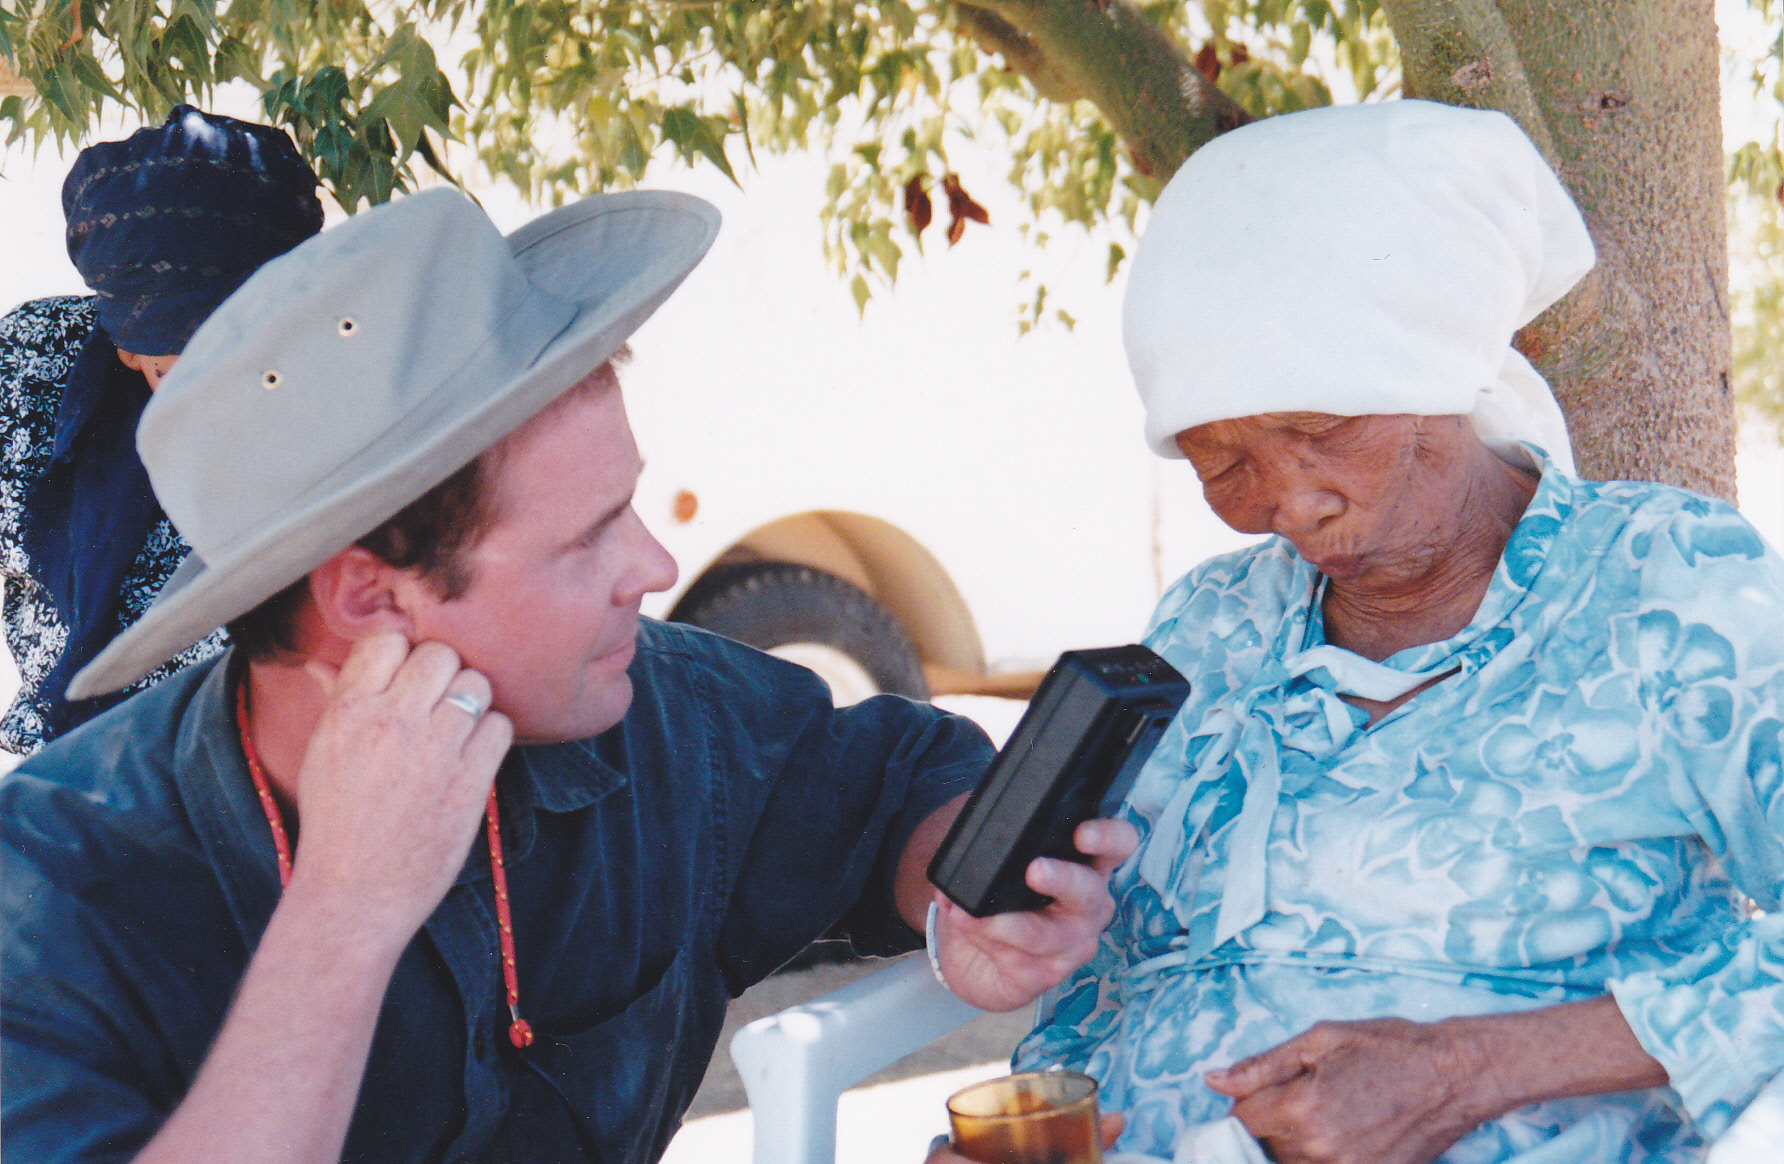
\includegraphics[width=.8\textwidth]{vaalbooi.jpg}\\
Nigel Crawhall, Elsie Vaalbooi (1997)\footnote{Photo credit:
Kalahari-Archive\_0050,  \textipa{\textdoublebarpipe}Khomani San
\textipa{\textvertline} Hugh Brody collection,
University of Cape Town Libraries, Special Collections.}
\end{center}

\newpage

%%%%%%%%%%%%%%%%%%%%%%%%%%%%%%%%%%%%%%%%%%%%%%%%%%%%%%%%%%%%%%%%%%%%%%%%%%%%%%%%

\markboth{}{}
\section{Voorwoord}
\markboth{}{}

In 1995, tydens ons eerste ontmoeting, het David Kruiper, die
tradisionele leier, vir my gevra om na die `ou'-taal te help soek. Met
Suid-Afrika in die aanvang van 'n nuwe demokratiese bedeling, het die
Kruiper-familie 'n grondeis ingestel om die Saasi-grondgebied wat
hulle in koloniale tyd verloor het, terug te kry. Sou die `ou'-taal
herwin word, kon dit as deurslaggewende bewys dien vir grondherstel.
Kort hierna het Roger Chennels, die gemeenskap se advokaat, gebel om
te s\^{e} 'n man op Rietfontein, ene Petrus Vaalbooi, vertel dat sy
ma, Elsie, die `ou'-taal praat.\\

In die bloedige somerhitte, met Tony Traill se CD \emph{Extinct:
Khoisan Languages of South Africa} by my, het ek Rietfontein toe gery.
Ons het in die yl koeltetjie van 'n doringboom op die Vaalboois se
werf ontmoet. Elsie het 'n blou blommetjierok en wit kopdoek gedra.
Haar o\"{e} was swak en sy was onseker waaroor die bohaai gaan. Toe
ons egter die snit op die CD speel waar 'n jong Saasi-vrou van haar
\emph{hokmeisie} - die gevierde oorgang na vrouwees - vertel, het tyd
verval.  Elsie was skielik vol lewe en 'n diep glimlag het oor haar
lippe gesprei. Sy het die woorde van hierdie vergange taal - haar
taal, haar storie - begin verduidelik. 'n Nuwe fase van Suid-Afrika se
geskiedenis het begin ontvou. Sy het ons aan die woord
\emph{n\textipa{\textvertline}uu} voorgestel. Dit beteken `om jou eie
taal te praat'.\\

Petrus Vaalbooi het dit sy missie gemaak om ander sprekers, wat
kol-kol oor die Kalahari-gebied versprei was, op te spoor. Ons het
altesaam 28 sprekers van N\textipa{\textvertline}uu, die taal wat vir
dekadeslank stil en onsigbaar was, ge\"{\i}dentifiseer. Ons het die
Kalahari-streek van woongebiede na verafgele\"{e} plase deurkruis om
die ryk taalerfenis na die gemeenskap en na die nasie terug te bring.
Die storie het die verbeelding van die land en van Thabo Mbeki, wat
toe president van die Republiek was, aangegryp.\\

Hierdie woordeboek verteenwoordig die uitstaande erfenis vir die
\textipa{\textdoublebarpipe}Khomani mense, vir inheemse mense van die
streek, vir Suid-Afrikaners en vir die mensegeslag in geheel. Dit val
saam met die aanvang van die Verenigde Nasies se Internasionale Dekade
van Inheemse Tale (2022--2032), 'n w\^{e}reldwye onderneming om 'n
ommeswaai in taalverlies teweeg te bring en alle pogings aan te wend
vir die bemagtiging van nuwe taalgebruikers.\\

Inheemse tale, insluitende di\'{e} wat nie meer vlot gepraat word nie,
is 'n kosbare hulpbron om ons verhouding met die w\^{e}reld en plekke
soos die Suidelike Kalahari te verstaan en om hulde te bring aan die
geslagte mense wat die mitologie, waardes en wysheid van hierdie
oeroue kultuur gevorm en oorgedra het. Ek wil my groot dank en respek
uitspreek teenoor die woordeboekspan en al die oudstes wat tot hierdie
geskiedkundige projek bygedra het.\\

Nigel Crawhall\\[1em]

Afdelingshoof, Plaaslike en Inheemse Kennisstelsels, UNESCO\\[1em]

13 Junie 2022

\vfill

\begin{center}
    %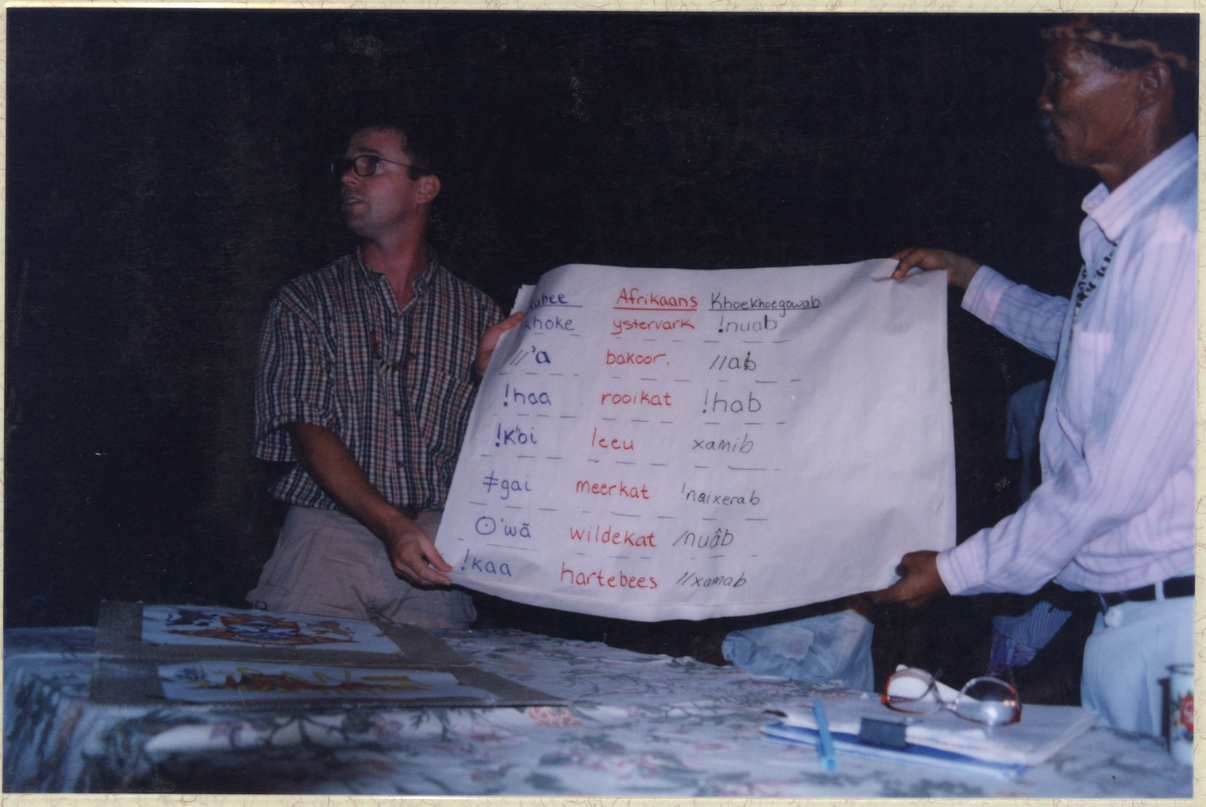
\includegraphics[width=.7\textwidth]{crawhall_petrus_vaalbooi.jpg}\\
    \includegraphics[width=.6\textwidth]{Enlarged_lam-36_Lightened.png}\\
    Nigel Crawhall, Petrus Vaalbooi (1997)\footnote{Photo credit: lam
    36, \textipa{\textdoublebarpipe}Khomani San $|$ Hugh Brody
    collection, University of Cape Town Libraries, Special
    Collections.}
\end{center}

\newpage

%%%%%%%%%%%%%%%%%%%%%%%%%%%%%%%%%%%%%%%%%%%%%%%%%%%%%%%%%%%%%%%%%%%%%%%%%%%%%%%%

\markboth{}{}
\addtocounter{section}{-1}
\tocless\section{Foreword}
\phantomsection
\addcontentsline{toc}{section}{\numberline {\thesection}Foreword}
\markboth{}{}

At our first meeting in 1995, traditional leader, Dawid Kruiper, asked
me if I would help look for the `old' language. With South Africa
entering a new democratic dispensation, the Kruiper family had
initiated a land claim to gain back Saasi territory lost in colonial
times. If this `old' language could be recovered, it would be vital
for achieving evidence for land restitution. Soon thereafter,
community lawyer, Roger Chennells phoned to say that a man in
Rietfontein, Petrus Vaalbooi, had come forth to say that his mother
Elsie spoke the `old' language.\\

I travelled up to Rietfontein in the heat of summer with Tony Traill's
CD \emph{Extinct: Khoisan Languages of South Africa}. We met in the
Vaalbooi's garden in the meagre shade of an acacia tree. Elsie wore a
blue floral dress and a white headscarf. Her eyes were weak and she
was not sure what the fuss was about. When we played the track from
the CD about a young Saasi woman recounting her \emph{hokmeisie}
celebration, the honoured transition into womanhood, suddenly time
fell away. Elsie was filled with life and a deep smile spread across
her lips. She began to explain the words of this distant language, her
language, her story, and a new phase of South African history began to
unfurl. She introduced us to the word
\emph{n\textipa{\textvertline}uu}, meaning `to speak one's own
language'.\\

Petrus Vaalbooi made it his mission to identify other speakers dotted
around the Kalahari territory. In all we were able to identify 28
speakers of N\textipa{\textvertline}uu, a language that had been
silent and invisible for decades. From townships to remote farms, we
criss-crossed the Kalahari, bringing this rich linguistic heritage
back to the community and back to the nation. The story captured the
imagination of the country and of the then President of the Republic,
Thabo Mbeki.\\

This dictionary represents an outstanding heritage for the
\textipa{\textdoublebarpipe}Khomani people, for indigenous peoples
regionally, for South Africans and for the human family. It comes as
the United Nations commences the International Decade of Indigenous
Languages (2022--2032), a worldwide initiative to turn the tide on
language loss and make all efforts to empower a new generation of
language users. Indigenous languages, including those not spoken
fluently today, are a precious resource for understanding our
relationship with the world, with places such as the southern
Kalahari, and to render homage to the generations of people who shaped
and transmitted the mythology, values and wisdom of this ancient
culture. I wish to express my great thanks and respect to the
dictionary team and to all of the elders who contributed to this
historic project.\\

Nigel Crawhall\\[1em]

Chief of Section, Local and Indigenous Knowledge Systems,
UNESCO\\[1em]

13 June 2022

\vfill
\begin{center}
    %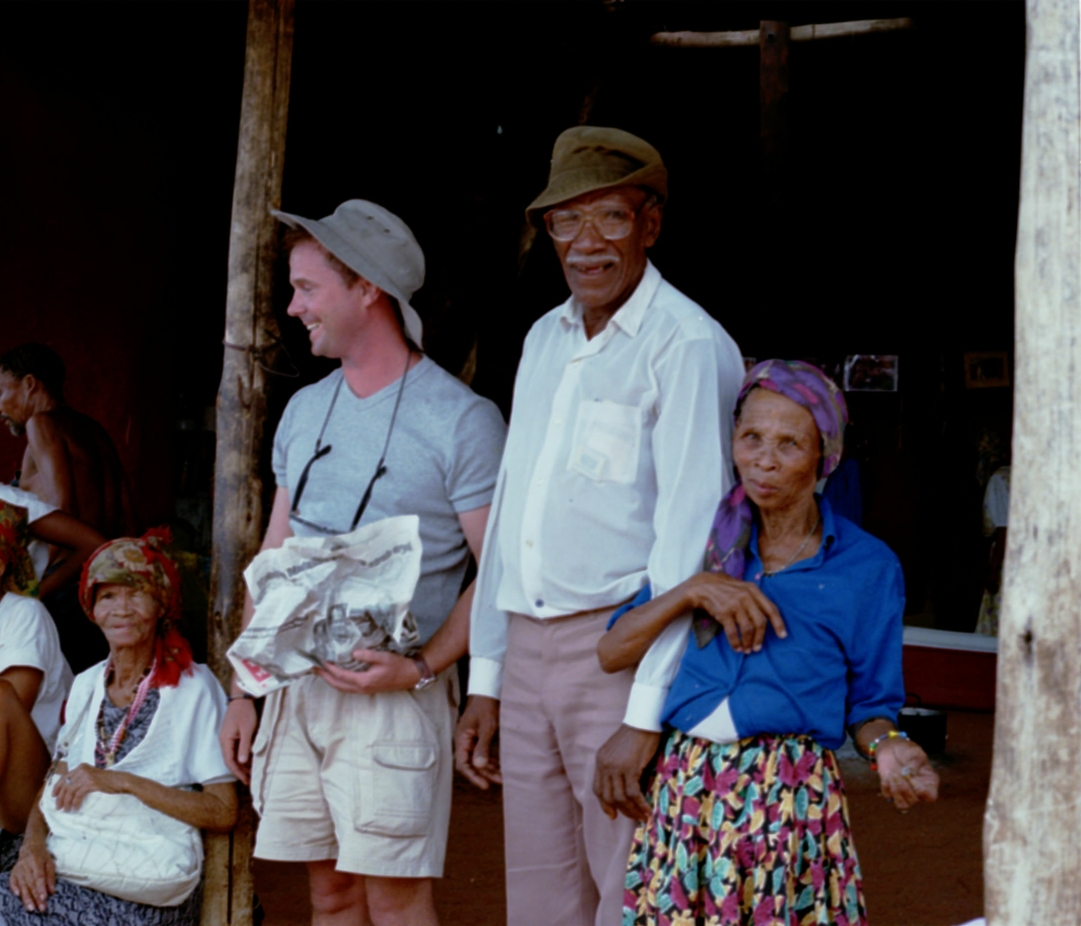
\includegraphics[width=.5\textwidth]{kruiper_koper_crawhall_olyn_swartz_crop.jpg}\\
    \includegraphics[width=.6\textwidth]{Enlarged_Neg_Colour_12-20_Lightened.png}\\
    Agtergrond: Dawid Kruiper, onbekend met rug na kamera, Kallais
    Kruiper, Lydia (Lys) Kruiper, Vytjie \textipa{\textvertline}Abaka
    Koper, Nigel Crawhall, Andries Olyn, Anna Swartz
    (1997)\footnote{\label{nc}Photo credit: Neg\_Colour\_12-20,
    \textipa{\textdoublebarpipe}Khomani San $|$ Hugh Brody collection, University of Cape Town
    Libraries, Special Collections.}\\
Background: Dawid Kruiper, unknown with back to camera, Kallais
    Kruiper, Lydia (Lys) Kruiper, Vytjie \textipa{\textvertline}Abaka
    Koper, Nigel Crawhall, Andries Olyn, Anna Swartz
    (1997)\footref{nc}
\end{center}


\newpage

%%%%%%%%%%%%%%%%%%%%%%%%%%%%%%%%%%%%%%%%%%%%%%%%%%%%%%%%%%%%%%%%%%%%%%%%%%%%%%%%

\markboth{}{}
\section{Vooraf}
\markboth{}{}

Die N\textipa{\textvertline}uu-taal is 'n lewende getuienis van 'n
diep geskiedenis en uithouvermo\"{e} van die mense wat op die
suidelike grense van die Kalahari-woestyn woon. Die klanke en
strukture van die taal is verstommend en ook baie mooi. Ons hoop dat
hierdie woordeboek sal help om die taalkundige genialiteit van die
Saasi-mense te demonstreer.\\

Ons is trots om die eerste groot publikasie wat
N\textipa{\textvertline}uu, Suid-Afrikaanse Nama, Noord-Kaap-Afrikaans
en Engels bymekaarbring, aan te bied. Hierdie werk beklemtoon die ryk
taalkundige- en kultuurgeskiedenis van die Noord-Kaap in Suid-Afrika.
Ons het hierdie tale met klank- en beeldopnames gedokumenteer. Die
opnames is gratis aanlyn beskikbaar. Die meertaligheid van hierdie
woordboek is 'n refleksie van die konteks waarin hierdie tale voorkom
- waar sprekers in hul daaglikse lewe die tale meng en daaraan 'n eg
Suid-Afrikaanse geurtjie verleen!\\

Ons het dit geweldig geniet om by die oudstes oor die
N\textipa{\textvertline}uu-taal te leer. Hulle is Anna (Antjie)
Kassie, Griet Seekoei, Katrina Esau, Hannie Koerant, Andries Olyn,
Hanna Koper, Vytjie \textipa{\textvertline}Abaka Koper, Simon Sauls,
\textipa{\textvertline}Una Rooi, Kheis Brou and Elsie Vaalbooi. Daar
is geen manier om genoeg dankie te s\^{e} dat hulle dit met ons gedeel
het nie. Dit het ons in staat gestel om dit nou hier met u te deel.\\

Die N\textipa{\textvertline}uu-taal is 'n taalkundige skat en ons hoop
dat u net soveel waarde daaraan heg soos ons.\\[1em]

\hfill Bonny Sands en Kerry Jones

\markboth{}{}
\addtocounter{section}{-1}
\tocless\section{Preface}
\phantomsection
\addcontentsline{toc}{section}{\numberline {\thesection}Preface}
\markboth{}{}

The N\textipa{\textvertline}uu language is a living testament to the
deep history and resilience of the people living at the southern edge
of the Kalahari desert. The sounds and structures of the language are
both astounding and beautiful. We hope this dictionary will help
showcase the linguistic genius of the Saasi people.\\

We are so proud to present the first major publication which brings
together N\textipa{\textvertline}uu, South African Nama, Northern Cape
Afrikaans and English. This work highlights the rich linguistic and
cultural heritage of the Northern Cape of South Africa. We have
documented these languages with audio and video recordings which can
be accessed online for free. The multilingual nature of this
dictionary reflects the context in which these languages occur, where
speakers use a mixture of languages in their daily lives - a truly
South African flavour!\\

We so much enjoyed learning about the N\textipa{\textvertline}uu
language from the elders: Anna (Antjie) Kassie, Griet Seekoei, Katrina
Esau, Hannie Koerant, Andries Olyn, Hanna Koper, Vytjie
\textipa{\textvertline}Abaka Koper, Simon Sauls,
\textipa{\textvertline}Una Rooi, Kheis Brou and Elsie Vaalbooi. We
cannot begin to sufficiently thank them for sharing it with us and
enabling us to share it with you.\\

The N\textipa{\textvertline}uu language is a linguistic treasure and
we hope you value it as much as we do.\\[1em]

\hfill Bonny Sands and Kerry Jones
\vspace{.8cm}

\makeatletter
\begin{center}
\begin{tabular}{ll}
    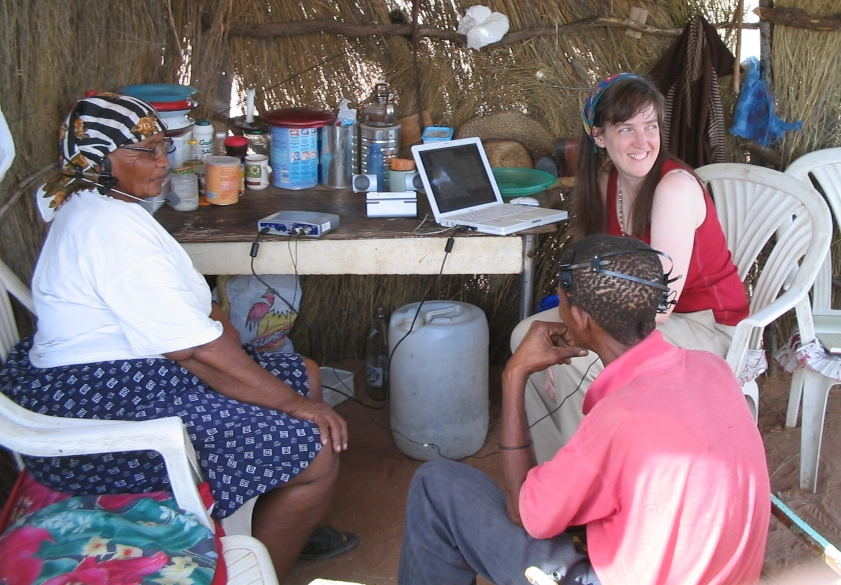
\includegraphics[height=5.5cm]{seekoei_sands_sauls_crop.jpg} &
    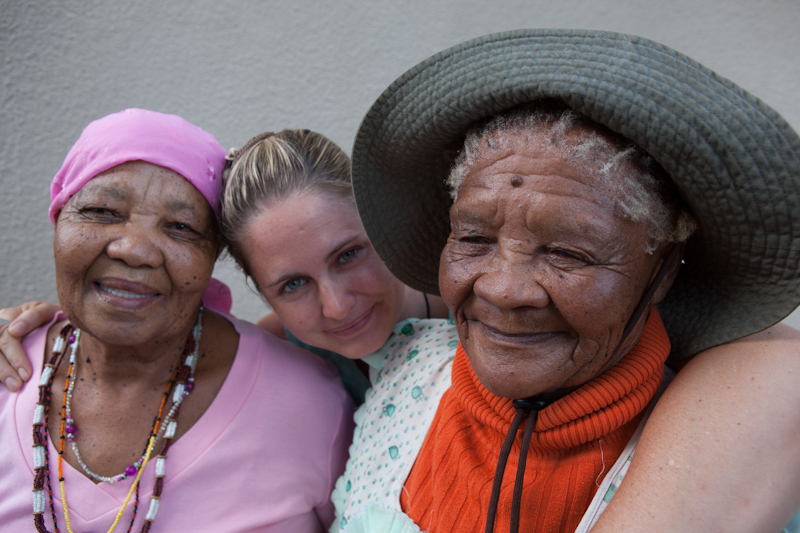
\includegraphics[height=5.5cm]{esau_jones_koper.jpg} \\
       Griet Seekoei, Bonny Sands, Simon Sauls
       (2006)\footnotemark\global\let\saved@Href@BS\Hy@footnote@currentHref
       &
       Katrina Esau, Kerry Jones, Hanna Koper
       (2015)\footnotemark\global\let\saved@Href@PW\Hy@footnote@currentHref
\end{tabular}
\end{center}
\addtocounter{footnote}{-1}
\let\Hy@footnote@currentHref\saved@Href@BS
\footnotetext{Photo credit: Becky Sands as provided by Bonny Sands.\label{bs}}
\stepcounter{footnote}
\let\Hy@footnote@currentHref\saved@Href@PW
\footnotetext{Photo credit: Paul Weinberg,
    \textipa{\textdoublebarpipe}Khomani San $|$ Hugh Brody collection,
    University of Cape Town Libraries, Special Collections.}
\makeatother


\newpage

%%%%%%%%%%%%%%%%%%%%%%%%%%%%%%%%%%%%%%%%%%%%%%%%%%%%%%%%%%%%%%%%%%%%%%%%%%%%%%%%

\markboth{}{}
\section{Vroe\"{e} dokumentasie van N\textipa{\textvertline}uu}
\markboth{}{}

Vroe\"{e} navorsers en ontdekkingsreisigers het gesukkel om hierdie
uitdagende taal te beskryf. Name en etikette wat hulle gebruik het,
het \textipa{\textdoublevertline}\textipa{N}, Langeberg\footnote{Neem
kennis dat hierdie term na die Langeberg in die Noord-Kaap verwys en
nie die Langeberge in die Wes-Kaap nie.} Bushmen,
\textipa{\textdoublebarpipe}Kaurure\textipa{\textdoublevertline}nai,
N\textipa{\textvertline}usa, \textipa{\textdoublevertline}\textipa{N}
!ke, S2, SIa, SIIa, Gemsbok Park, N\textipa{\textvertline}huki,
N\textipa{\textvertline}hu en \textipa{\textdoublebarpipe}khomani
ingesluit.  Die term N\textipa{\textdoublevertline}ng is die tegniese
etiket vir hierdie dialekgroepering, maar ons gebruik die term
N\textipa{\textvertline}uu hier omdat lede van die gemeenskap dit so
gebruik in hul pogings om die taal te laat herleef.  Die eerste poging
om N\textipa{\textvertline}uu-woorde neer te skryf, was waarskynlik
deur Lucy Lloyd in 1885 maar, ongelukkig het haar oorspronklike
aantekeninge verlore geraak (kruisverw.\
\cite{Gueldemann2017})\footnote{Verwys na hierdie referaat vir 'n
gedetailleerde uiteensetting van die vroe\"{e} dokumentasie van die
N\textipa{\textdoublevertline}ng-vari\"{e}teite.}. Twee
ontdekkingsreisigers, Heinrich Pabst en Rudolf P\"{o}ch, het ook
enkele woorde neergeskryf en hulle kon selfs klankopnames gemaak het,
maar hierdie is tot dusver ontoeganklik. Lucy Lloyd se susterskind,
Dorothea Bleek, het meestal tussen 1901 en 1911 veldwerk rondom die
taal gedoen en hierdie aantekeninge is vandag - saam met baie meer
uitgebreide dokumentasie van \textipa{\textvertline}Xam, 'n verwante
taal - deel van die Digitale Bleek en Lloyd Versameling by die
Universiteit van Kaapstad. Crawhall se Ph.D-proefskrif beskryf die
proses van taalverskuiwing wat onder !Ui-Taa-sprekers van die
Gordonia- en Postmasburg distrikte van Suid-Afrika, plaasgevind het.
\parencite{Crawhall2004}.\\

Die vroegste klankopnames van N\textipa{\textvertline}uu waartoe ons
toegang gehad het, is in 1936 deur lede van 'n wetenskapsending na die
Kalahari op wassilinders gemaak en in 1999 deur Tony Traill
gedigitaliseer.  Clement Doke en L.\ F.\ Maingard het as een van die
uitkomste van hierdie sending, belangrike vroe\"{e} werk oor die taal
gepubliseer.  'n Hele paar dekades later het Ernst Westphal
bandopnames gemaak wat ook gedigitaliseer is en aanlyn by die
Universiteit van Kaapstad beskikbaar is. Toe Tony Traill in 1973 geen
sprekers van die taal in die Kalahari Gemsbokpark kon kry nie, is daar
gedink dat die taal uitgesterf het\ldots


\markboth{}{}
\addtocounter{section}{-1}
\tocless\section{Early documentation of N\textipa{\textvertline}uu}
\phantomsection
\addcontentsline{toc}{section}{\numberline {\thesection}Early
documentation of N\textipa{\textvertline}uu}
\markboth{}{}

Early researchers and explorers grappled with describing this
challenging language. Names and labels that they used included:
\textipa{\textdoublevertline}\textipa{N}, Langeberg\footnote{Note that
this term refers to the Langeberg Mountain of the Northern Cape and not
the Langeberg Mountains of the Western Cape.} Bushmen,
\textipa{\textdoublebarpipe}Kaurure\textipa{\textdoublevertline}nai,
N\textipa{\textvertline}usa, \textipa{\textdoublevertline}\textipa{N}
!ke, S2, SIa, SIIa, Gemsbok Park, N\textipa{\textvertline}huki,
N\textipa{\textvertline}hu and \textipa{\textdoublebarpipe}khomani.
The term N\textipa{\textdoublevertline}ng is the technical label for
this dialect cluster but we use the term N\textipa{\textvertline}uu
here because it is used by community members in their revitalisation
efforts.  The first attempt made at writing N\textipa{\textvertline}uu
words was probably around 1885 by Lucy Lloyd, but unfortunately her
original notes have been lost (cf.\
\cite{Gueldemann2017})\footnote{Please refer to this paper for a
detailed account of the early documentation of
N\textipa{\textdoublevertline}ng varieties.}. Explorers Heinrich Pabst
and Rudolf P\"{o}ch also recorded a few words and perhaps even made
audio recordings, though these are as of yet, inaccessible. Lucy
Lloyd's niece, Dorothea Bleek conducted fieldwork on the language
mostly between 1901 and 1911, and these notes can be seen today at the
Digital Bleek and Lloyd Collection at the University of Cape Town,
along with much more extensive documentation of
\textipa{\textvertline}Xam, a related language.\\

The earliest audio recordings of N\textipa{\textvertline}uu that we
have been able to access were those made on wax cylinders by members
of a scientific expedition to the Kalahari in 1936 that were digitised
by Tony Traill in 1999. Clement Doke and L.\ F.\ Maingard published
important early works on the language as a result of this expedition.
Several decades later, Ernst Westphal made tape recordings of the
language which have also been digitised and are available online at
the University of Cape Town. When Tony Traill was unable to find
speakers of the language in the Kalahari Gemsbok Park in 1973, the
language was thought to be extinct\ldots
\vspace{.5cm}

\begin{center}
    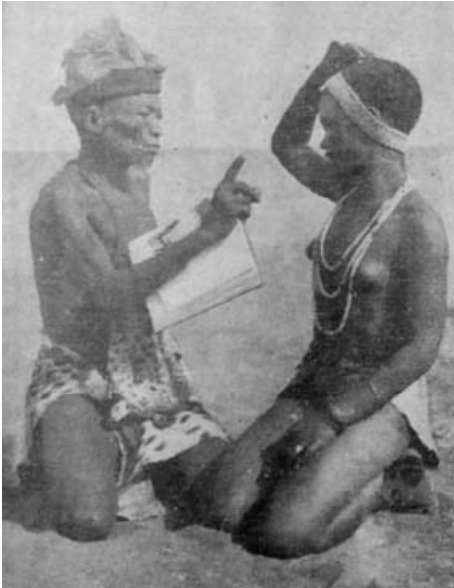
\includegraphics[height=5.5cm]{abraham_janake_bwav.png}\\
    Ou Abraham, Klein Janake (1936)\footnote{Photo credit: Rand Daily
    Mail, 1936.}
\end{center}

\newpage

%%%%%%%%%%%%%%%%%%%%%%%%%%%%%%%%%%%%%%%%%%%%%%%%%%%%%%%%%%%%%%%%%%%%%%%%%%%%%%%%

\markboth{}{}
\section{N\textipa{\textvertline}uu-herlewingsverhaal}
\markboth{}{}

Hedendaagse werk oor N\textipa{\textvertline}uu het, na die taal in in
1995 herontdek is, plaasgevind. Die Kanadese taalkundige, Nigel
Crawhall het saam met Tony Traill 'n kort woordelys van die taal
gedokumenteer en hy en ander het baie video-opnames gemaak. Di\'{e} is
aanlyn beskikbaar as deel van die \textipa{\textdoublebarpipe}Khomani
San $|$ Hugh Brody-Versameling by die Universiteit van Kaapstad.
Crawhall se Ph.D-proefskrif beskryf die proses van taalverskuiwing wat
onder !Ui-Taa-sprekers van die Gordonia- en Postmasburg distrikte van
Suid-Afrika, plaasgevind het \parencite{Crawhall2004}.
Levi Namaseb van die Universiteit van Namibi\"{e} het begin om
'n ortografie (spelstelsel) te skep van die taal wat in werklikheid
nog in 1998 deur lede van die gemeenskap gebruik is. Hy het ook gehelp
om kinders die taal te leer praat en skryf.
In 2006 het Namaseb sy Ph.D-proefskrif, wat
\textipa{\textdoublebarpipe}Khomani storievertelling in Nama,
N\textipa{\textvertline}uu, Afrikaans en Engels bevat, voltooi
\parencite{Namaseb2006}.
Van 2000--2002 het Tom G\"{u}ldemann 'n taalwerkskets
\parencite{Gueldemannforthcoming2003}\footnote{Hierdie werk is
ondersteun deur die Duitse Navorsingstigting (DFG) toegif GU 400/1-1:
\emph{Genetic and typological profile of the Tuu language family:
Inventarisation and linguistic analysis of existing sources},
uitgevoer van 10/2000--4/2002.} wat op Westphal se veldwerk baseer is,
voortgebring en in 2003 het hy vir Mats Exter Upington toe gevat om
aan die taal te begin werk.  Mats Exter (met steun van die Duitse
Akademiese Uitruildiens (DAAD) en die Universiteit van Keulen) se
navorsing wat hy van 2003--2005 oor die taal gedoen het, het in 2008
die grondslag van sy Ph.D-proefskrif gevorm.\\

Later het die Amerikaanse navorsers, Chris Collins, Amanda Miller,
Bonny Sands en Johanna Brugman, by Levi Namaseb aangesluit.  Hulle het
vanaf 2003--2007 met die steun van die VS se Nasionale
Wetenskapstigting veldwerk gedoen. Hierdie VSA/Namibiese samewerking
het 'n aantal artikels en 'n grammatika \parencite{Collins2011}
opgelewer, asook die klankargief waarop die grammatika en hierdie
woordeboek gebaseer is.  Vanaf 2007, met die steun van die
Bedreigdetale-dokumentasieprogram (ELDP), het 'n afsonderlike span
navorsers (Alena Witzlack-Makarevich, Tom G\"{u}ldemann, Sven
Siegmund, Martina Ernszt-Shaw) wat in Duitsland gebaseer was, begin
met werk oor die taal. In hul wetenskaplike verslae word na die
Oostelike dialek van die taal verwys as
N\textipa{\textdoublevertline}ng, en die Westelike dialek word
N\textipa{\textvertline}uu genoem, soos in hul klankargief wat in die
Bedreigdetale-argief (ELAR) gehuisves word.\\

Meer onlangse werk oor N\textipa{\textvertline}uu het gefokus op die
produksie van storieboeke en leerstof. Met behulp van 'n voor\-lopige
weergawe van hierdie woordeboek en gepubliseerde navorsing, is twee
N\textipa{\textvertline}uu-leesboekies (om die taal aan te leer)
geskep: een in 2013 deur Ariel Appel, 'n student by die Hebreeuse
Universiteit in Jerusalem, en 'n ander in 2016 deur Sheena Shah en
Matthias Brenzinger, toe geaffilieer met die Universiteit van
Kaapstad.  Hierdie navorsers kon slegs direk met een spreker van
N\textipa{\textvertline}uu, Katrina Esau, saamwerk.  Die
Suid-Afrikaanse San-Instituut (SASI) het in 2012 die boek \emph{Ek is
Spesiaal/Na ng Spesiaal: Afrikaans/N\textipa{\textvertline}uu}
geproduseer. In 2014 het 'n nieregeringsorganisasie genaamd
\textipa{\textdoublebarpipe}Khomani Maatskaplike-ontwikkelingsgroep
(KhomSoDev) 'n leesboekie met die titel \emph{Ek kan
N\textipa{\textvertline}uuki, praat, lees en skryf/I can speak, read
and write N\textipa{\textvertline}uuki}, geproduseer. Dit is gebaseer
op 'n ongepubliseerde leesboekie deur Levi Namaseb en die Amerikaanse
taalkundiges wat hierbo genoem word. Ouma Katrina Esau en haar
kleindogter, Claudia Snyman, het met die Puku Kinderliteratuurstigting
saamgewerk om die boek \emph{!Qhoi n\textipa{\textvertline}a
Tjhoi/Skilpad en Volstruis/Tortoise and Ostrich}, te produseer. Dit is
in 2021 gepubliseer.\\

Hierdie woordeboek is gebaseer op uitgebreide digitale klankopnames
van twee onderskeie dialekte van die N\textipa{\textvertline}uu-taal.
Dit word hier Oostelik en Westelik genoem. (Let egter op dat dit lyk
asof daar in die verlede nog ander dialekte kon gewees het). Die
meerderheid van die woorde in di\'{e} woordeboek is deur die
VSA/Namibiese navorsers opgeneem. Hulle het 'n metodologie van direkte
ontlokking gebruik om dit te doen. Dit beteken dat daar in Afrikaans
vrae soos `Hoe s\^{e} jy kat?' aan 'n groep
N\textipa{\textvertline}uu-sprekendes sal vra en hulle tipies in 'n
mengsel van Afrikaans en N\textipa{\textvertline}uu byvoorbeeld sal
antwoord \emph{Ek s\^{e} m\textipa{\!o}oa}. Sommige woorde was maklik
om te vertaal, maar ander moes bevestig word deur die gebruik van
fotos, beskrywings of lang besprekings. N\'{a} die bevestiging van 'n
klompie woorde, sou di\'{e} navorsers dan die teikenwoorde opneem in
die raamsin `Ek s\^{e} \underline{\hspace{1cm}}.' (\emph{Na ka}
\underline{\hspace{1cm}}.) en elkeen 3 maal per spreker herhaal.
Navorsers het gepoog om elke woord met sowel Oostelike as Westelike
dialeksprekers op te neem. Die beperkte beskikbaarheid van
eersgenoemde het egter beteken dat hulle nie altyd daarin geslaag het
nie.\\

Die tweede hoofbron van woordeboekinskrywings was opnames wat deur
dr.\ Kerry Jones van African Tongue\footnote{Soos befonds deur die
Departement van Sport, Kuns en Kultuur (DSKK) van die Republiek van
Suid-Afrika, vir die projek \emph{Digitale Woordeboekhulpbronne vir
N\textipa{\textvertline}uu (Digital Dictionary Resources for
N\textipa{\textvertline}uu)} in antwoord op die oproep om \emph{Human
Language Technology Projects}.} gemaak is. Sy het dit in 2021--2022
met Katrina Esau en die hulp van lede van die
N\textipa{\textvertline}uu-Taalowerheid (NTO): Claudia Snyman, David
van Wyk en Sussie Bok, gedoen. Oor hierdie tydperk het Kerry verskeie
besoeke aan Upington gebring om N\textipa{\textvertline}uu-woorde weer
op te neem in die gevalle waar die oorspronklike klankl\^{e}er \'{o}f
van swak gehalte was, ontbreek het \'{o}f bederf was. Sy het ook nuwe
woorde van Ouma Katrina ontlok wat spesifiek verband hou met moderner
begrippe soos `toep' of `app', en `koronavirus (COVID-19)'. Bykomend
is 'n reeks van tien gemeenskapnuusbriewe deur African Tongue
saamgestel om projekvordering met gemeenskapslede te deel, insette te
lewer en terugvoer te verskaf. Woordelyste is ook ingesluit vir
verdere bevestiging. Deur hierdie proses is meer as 1000
N\textipa{\textvertline}uu-woorde digitaal opgeneem.\\

Sommige bykomende inskrywings is gebaseer op die dokumentasie van
sinne en stories deur VSA/Namibiese navorsers, Collins en
Namaseb, en ander is bygedra deur Witzlack-Makarevich uit die
uitgebreide opnames van on\-uit\-gelokte (d.w.s.\ natuurliker) spraak wat
sy, Tom G\"{u}ldemann, Sven Siegmund en Martina Ernszt-Shaw opgeneem
het. Bykomende woorde (veral plekname en mense se name) is bevestig
met gebruik van die video-opnames met bypassende
transkripsie-l\^{e}ers van die \textipa{\textdoublebarpipe}Khomani San
$|$ Hugh Brody-Versameling by die Universiteit van Kaapstad (UCT).
Hierdie versameling huisves foto's, getranskribeerde klank- en
videodata van die \textipa{\textdoublebarpipe}Khomani-mense en hul
tale. Meer as 300 transkripsies is tot dusver - van 2014 tot 2022 -
onder toesig van Kerry Jones van African Tongue gemaak en die proses
duur steeds voort. Toegang tot hierdie inhoud kan verkry word via
Kaapstad Universiteit se biblioteke, Spesiale Versamelings.\\

Al die klank- en teksdokumentasie wat in hierdie woordeboek gebruik
is, word gehuisves in 'n versameling by die Suid-Afrikaanse Sentrum
vir Digitale Taalhulpbronne (SADiLaR).
N\textipa{\textvertline}uu-opnames, Suid-Afrikaanse Nama en 'n
plaaslike vari\"{e}teit van Afrikaans wat onder die sprekers bekend
staan as \emph{Onse Afrikaans} of \emph{Ons Afrikaans}, is ingesluit.
Alle data wat tussen 2001 en 2022 ingesamel is, is plaaslik in
Upington, Askham en Witdraai in die Noord-Kaap van moeder\-taal\-sprekers
van die teikentale verkry. Nadat die span van African Tongue alle
opsies uitgeput en soveel moontlike uitstaande data ingesamel het en
inskrywings deur die N\textipa{\textvertline}uu-Taalowerheid bevestig
is, het die skoonmaak van die data begin. Onder leiding van Menno van
Zaanen van SADiLaR, 'n professor in Digitale Geesteswetenskap, en met
behulp van die span se taalredakteurs, is die finale verifi\"{e}ring
van elke inskrywing in al vier tale gedoen. 'n Rekenaarprogram om die
skoon datastel in 'n gesofistikeerde woordeboek soos hierdie
woordeboek te sit, is ontwikkel. Die inligting in die datastel is ook
omskep om toegang deur 'n webportaal en 'n selfoontoep moontlik te
maak. \mbox{Hierdie} is 'n trotse oomblik op ons lang reis om die uitsette
van ons navorsing so vrylik moontlik vir die algemene Suid-Afrikaanse
publiek toeganklik te maak met die klem op gebruikersvriendelikheid en
taalkundige omvattendheid.\\

Die deelname van gemeenskapslede, veral
\textipa{\textdoublebarpipe}Xuu\textipa{\textvertline}eeki Katrina
Esau, was die grondslag vir hierdie hele proses. Dit was 'n uiters
uitdagende, maar bevredigende taak en ons is gese\"{e}nd om na al die
jare se samewerking en harde werk die vrug van ons arbeid te sien.


\markboth{}{}
\addtocounter{section}{-1}
\tocless\section{N\textipa{\textvertline}uu revival story}
\phantomsection
\addcontentsline{toc}{section}{\numberline
{\thesection}N\textipa{\textvertline}uu revival story}
\markboth{}{}

Modern work on N\textipa{\textvertline}uu took place after the
`rediscovery' of the language in 1995. Canadian linguist Nigel
Crawhall documented a short word-list of the language along with Tony
Traill. Crawhall and others made many video recordings that are now
available online as part of the \textipa{\textdoublebarpipe}Khomani
San $|$ Hugh Brody Collection at the University of Cape Town.
Crawhall's Ph.D thesis described the process of language shift that
took place among !Ui-Taa speakers from the Gordonia and Postmasburg
Districts of South Africa \parencite{Crawhall2004}.  Levi Namaseb of the
University of Namibia began the work of creating
an orthography (spelling system) of the language that was actually
used by community members in 1998. He also helped children learn to
speak and write the language.
In 2006 Namaseb completed his Ph.D thesis which featured
\textipa{\textdoublebarpipe}Khomani
storytelling in Nama, N\textipa{\textvertline}uu, Afrikaans and English
\parencite{Namaseb2006}.
 From 2000--2002, Tom G\"{u}ldemann
produced a grammar sketch
\parencite{Gueldemannforthcoming2003}\footnote{This work was supported
by the German Research Foundation (DFG) grant GU 400/1-1: \emph{Genetic
and typological profile of the Tuu language family: Inventarisation
and linguistic analysis of existing sources} carried out
10/2000--4/2002.} based on Westphal's fieldwork and in 2003 took Mats
Exter to Upington to begin work on the language. Mats Exter (with
support from the German Academic Exchange Service (DAAD) and the
University of Cologne) did research on the language from 2003--2005,
which formed the basis of his 2008 Ph.D thesis.\\

Levi Namaseb was later joined by American researchers Chris Collins,
Amanda Miller, Bonny Sands and Johanna Brugman who conducted fieldwork
from 2003--2007 supported by the US National Science Foundation. This
USA/Namibian collaboration produced a number of articles and a grammar
\parencite{Collins2011}, as well as the audio archive on which the
grammar and this dictionary are based.  Beginning in 2007, with
support from the Endangered Languages Documentation Programme (ELDP),
a separate team of researchers based in Germany (Alena
Witzlack-Makarevich, Tom G\"{u}ldemann, Sven Siegmund, Martina
Ernszt-Shaw) began work on the language. In their scientific papers,
the Eastern dialect of the language is referred to as
N\textipa{\textdoublevertline}ng, and the Western dialect is called
N\textipa{\textvertline}uu, as in their audio archive housed at the
Endangered Languages Archive (ELAR).\\

More recent work on N\textipa{\textvertline}uu has focused on the
production of storybooks and language learning materials. With the
help of a draft version of this dictionary and published research, two
N\textipa{\textvertline}uu primers (language learning books) were
created, one by Ariel Appel, a student at the Hebrew University in
Jerusalem in 2013 and another in 2016 by Sheena Shah and Matthias
Brenzinger, then affiliated with the University of Cape Town. These
researchers were only able to work directly with one speaker of
N\textipa{\textvertline}uu, Katrina Esau. The South African San
Institute (SASI) produced the book \emph{Ek is Spesiaal/Na ng
Spesiaal: Afrikaans/N\textipa{\textvertline}u} in 2012. In 2014, an
non-governmental organisation called
\textipa{\textdoublebarpipe}Khomani Social Development Group
(KhomSoDev) produced a reader called \emph{Ek kan
N\textipa{\textvertline}uuki, praat, lees en skryf/I can speak, read
and write N\textipa{\textvertline}uuki}, based on an unpublished
primer by Levi Namaseb and the American linguists mentioned above.
Ouma Katrina Esau and her granddaughter Claudia Snyman collaborated
with the Puku Children's Literature Foundation to produce the book
\emph{!Qhoi n\textipa{\textvertline}a Tjhoi/Skilpad en
Volstruis/Tortoise and Ostrich}, published in 2021.\\

This dictionary is based on extensive digital audio recordings of two
distinct dialects of the N\textipa{\textvertline}uu language, labelled
here Eastern and Western. (Note however, that it seems that there may
have been additional dialects in the past.) The majority of the words
in this dictionary were recorded by the USA/Namibian researchers,
through a methodology of direct elicitation. In other words, we asked
groups of N\textipa{\textvertline}uu speakers questions in Afrikaans
such as `How do you say cat?' and they would typically reply in a mix
of Afrikaans and N\textipa{\textvertline}uu, e.g.\ \emph{Ek s\^{e}
m\textipa{\!o}oa}. Some words were easy to translate but others had to
be verified through the use of pictures, descriptions or long
discussions. After verifying a few dozen words, these researchers
would then record the target words in the frame sentence `I say
\underline{\hspace{1cm}}.' (\emph{Na ka} \underline{\hspace{1cm}}.),
repeated 3 times per speaker. Researchers attempted to record every
word with both Eastern and Western dialect speakers, but the limited
availability of the former meant that they did not always achieve
this.\\

The second major source of dictionary entries was from recordings made
by Dr.\ Kerry Jones from African Tongue\footnote{As funded by
Department of Sport, Arts and Culture (DSAC) of the Republic of South
Africa, for the project \emph{Digital Dictionary Resources for
N\textipa{\textvertline}uu} as a response to the call for \emph{Human
Language Technology Projects}.} in 2021--2022 with Katrina Esau and
the help of N\textipa{\textvertline}uu Language Authority (NLA)
members: Claudia Snyman, David van Wyk and Sussie Bok. Over this time
period, Kerry visited Upington several times to re-record
N\textipa{\textvertline}uu words in cases where the original sound
file was either of poor quality, missing or corrupt. She also elicited
new words from Ouma Katrina relating specifically to more modern
concepts such as `app', and `Coronavirus (COVID-19)'. Additionally, a
series of ten community newsletters were created by African Tongue to
share project progress with community members, provide input and
feedback as well as wordlists for further verification. Throughout
this process more than 1000 N\textipa{\textvertline}uu words were
digitally recorded.\\

Some additional entries are based on the documentation of sentences
and stories by USA/Namibian researchers Collins and Namaseb,
and others were contributed by Witzlack-Makarevich from the
extensive recordings of unelicited (i.e.\ more naturalistic) speech
made by her, Tom G\"{u}ldemann, Sven Siegmund and Martina Ernszt-Shaw.
Additional words (especially place names and names of people) were
verified using the video footage with matching transcript files from
the \textipa{\textdoublebarpipe}Khomani San $|$ Hugh Brody Collection
at the University of Cape Town (UCT). This collection houses
photographs, audio, video and transcript data featuring the
\textipa{\textdoublebarpipe}Khomani people and their languages. Over
300 transcripts have been created so far, this process was overseen by
Kerry Jones from African Tongue from 2014 to 2022 and is on-going;
this content can be accessed via UCT libraries, Special Collections.\\

All of the audio and textual documentation used in this dictionary is
housed in a collection at the South African Centre for Digital
Language Resources (SADiLaR). This includes N\textipa{\textvertline}uu
recordings, South African Nama and a local variety of Afrikaans known
by the speakers as \emph{Onse Afrikaans} or \emph{Our Afrikaans}. All
data collected between 2001 and 2022 were collected from mother tongue
speakers of the target languages on site in Upington, Askham and
Witdraai in the Northern Cape. Once the team from African Tongue had
exhausted all options and recorded as much outstanding data as
possible, and verified entries with the N\textipa{\textvertline}uu
Language Authority, the data cleaning process began. With the
direction of Menno van Zaanen from SADiLaR, a Digital Humanities
professor, and the help of the team's language editors, final
verification could be made for each entry in all four languages. A
computer program was developed that is used to convert the cleaned
dataset into a sophisticated dictionary found in the dictionary proper
of this publication. The information in the dataset was also converted
to allow access through a web-portal and a mobile phone app. A proud
moment in our long journey to make the outputs of our research
accessible to the general South African public and beyond as freely as
possible with a key focus on user-friendliness and linguistic
inclusion.\\

The participation of community members, most especially
\textipa{\textdoublebarpipe}Xuu\textipa{\textvertline}eeki Katrina
Esau was the foundation for this entire process. An especially
challenging but rewarding task that we are blessed to bring to
fruition after all these years of collaboration and hard work.\\

\makeatletter
\begin{center}
    \begin{tabular}{p{.4\textwidth}p{.4\textwidth}}
        \multicolumn{1}{c}{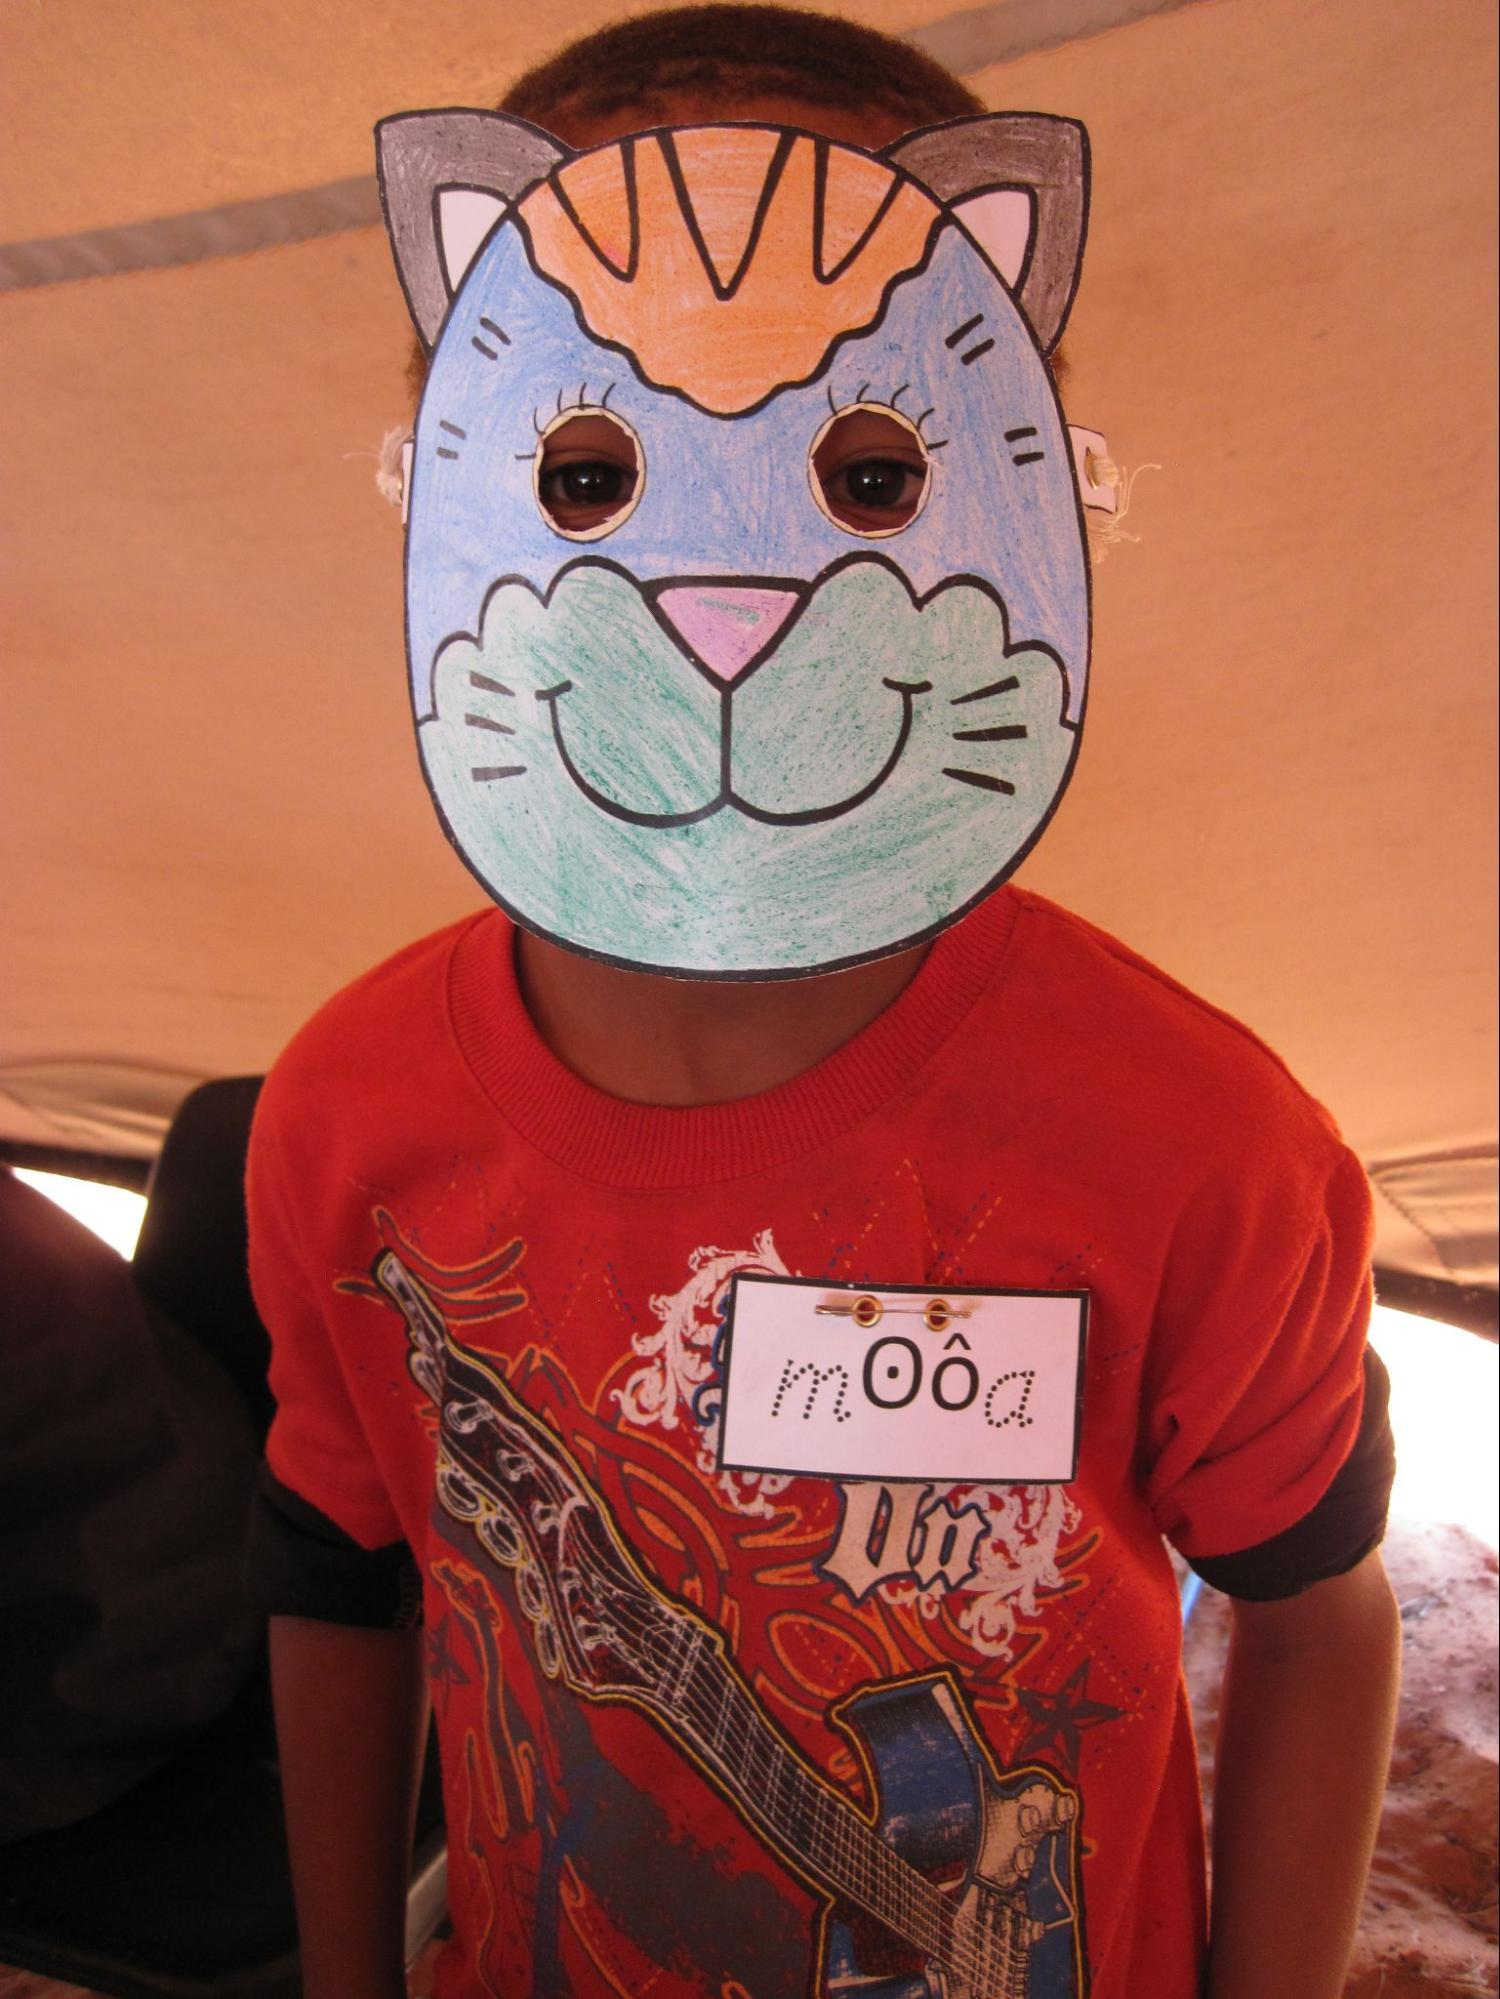
\includegraphics[width=.27\textwidth]{teaching.jpg}} & 
        \multicolumn{1}{c}{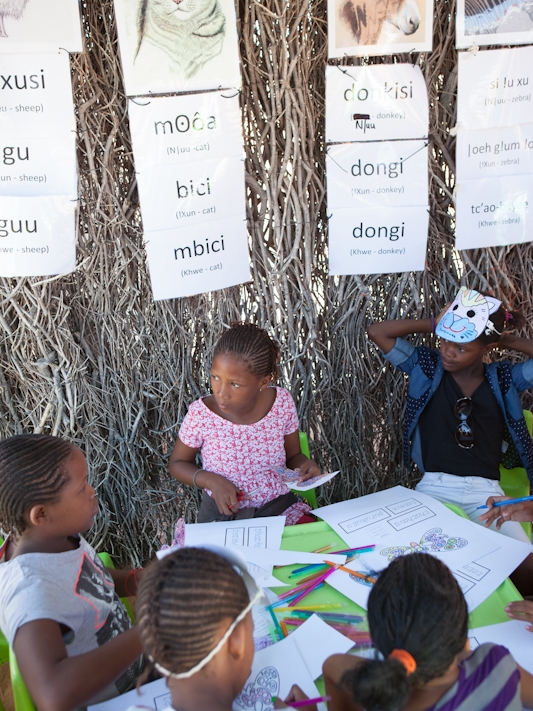
\includegraphics[width=.27\textwidth]{names_crop.jpg}} \\

        N\textipa{\textvertline}uu-lesse deur African Tongue, Kalahari
        Desert Festival (2014)\footnotemark\global\let\saved@Href@KJ\Hy@footnote@currentHref
        &
        Kinders leer diername in  N\textipa{\textvertline}uu, Khwe and !Xun saam met African
        Tongue, Kalahari Desert Festival
        (2014)\footnotemark\global\let\saved@Href@LE\Hy@footnote@currentHref \\

    Teaching and learning N\textipa{\textvertline}uu with African
        Tongue, Kalahari Desert Festival (2014)\footref{kj}
        &
        Learning N\textipa{\textvertline}uu, Khwe and !Xun animal
        names with African Tongue, Kalahari Desert Festival
        (2014)\footref{le}
        \\
    \end{tabular}\\[1em]

    \begin{tabular}{p{.4\textwidth}p{.4\textwidth}}
        \multicolumn{1}{c}{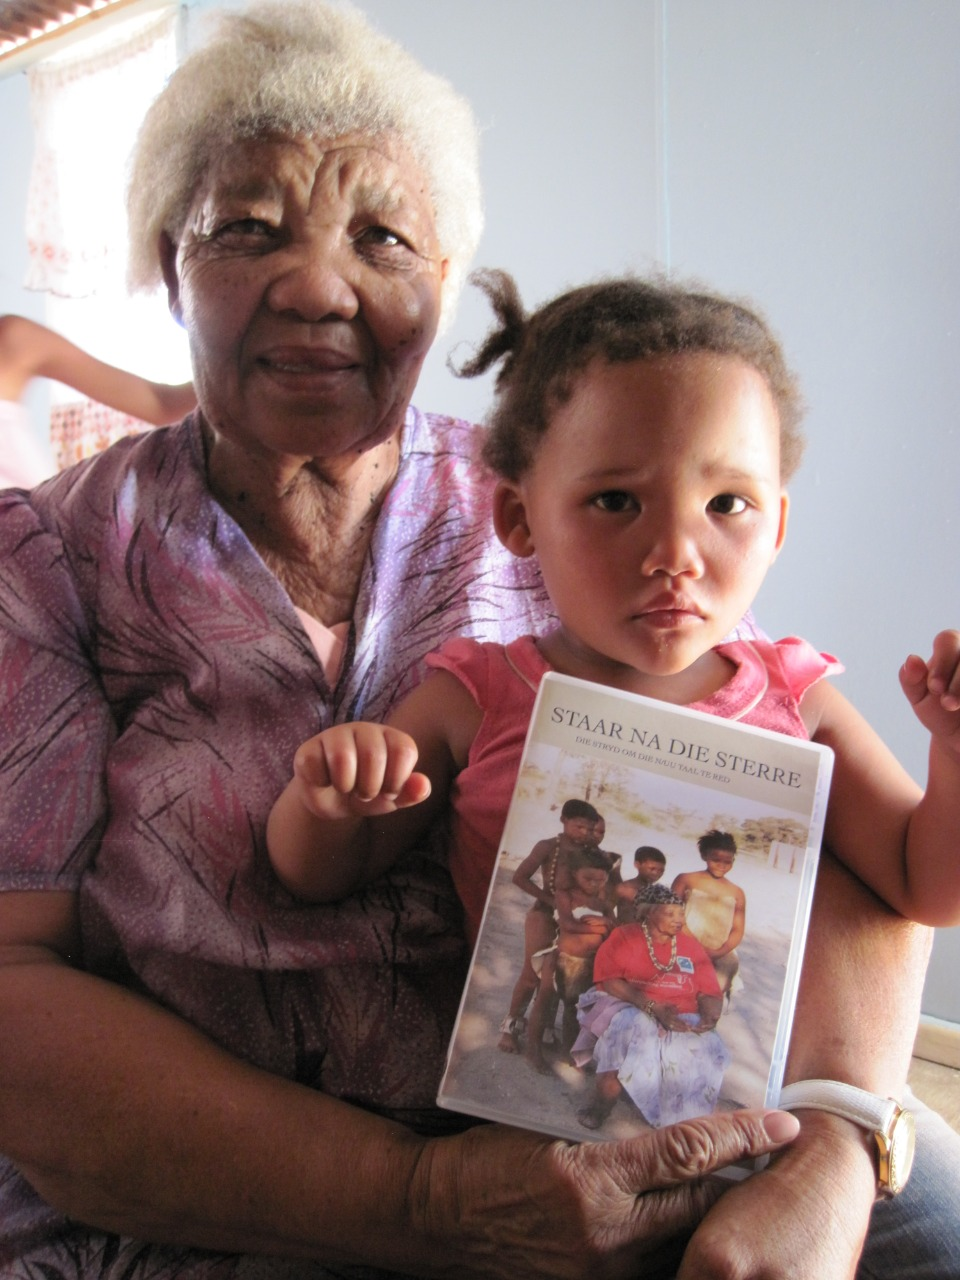
\includegraphics[width=.27\textwidth]{index.jpeg}} &
        \multicolumn{1}{c}{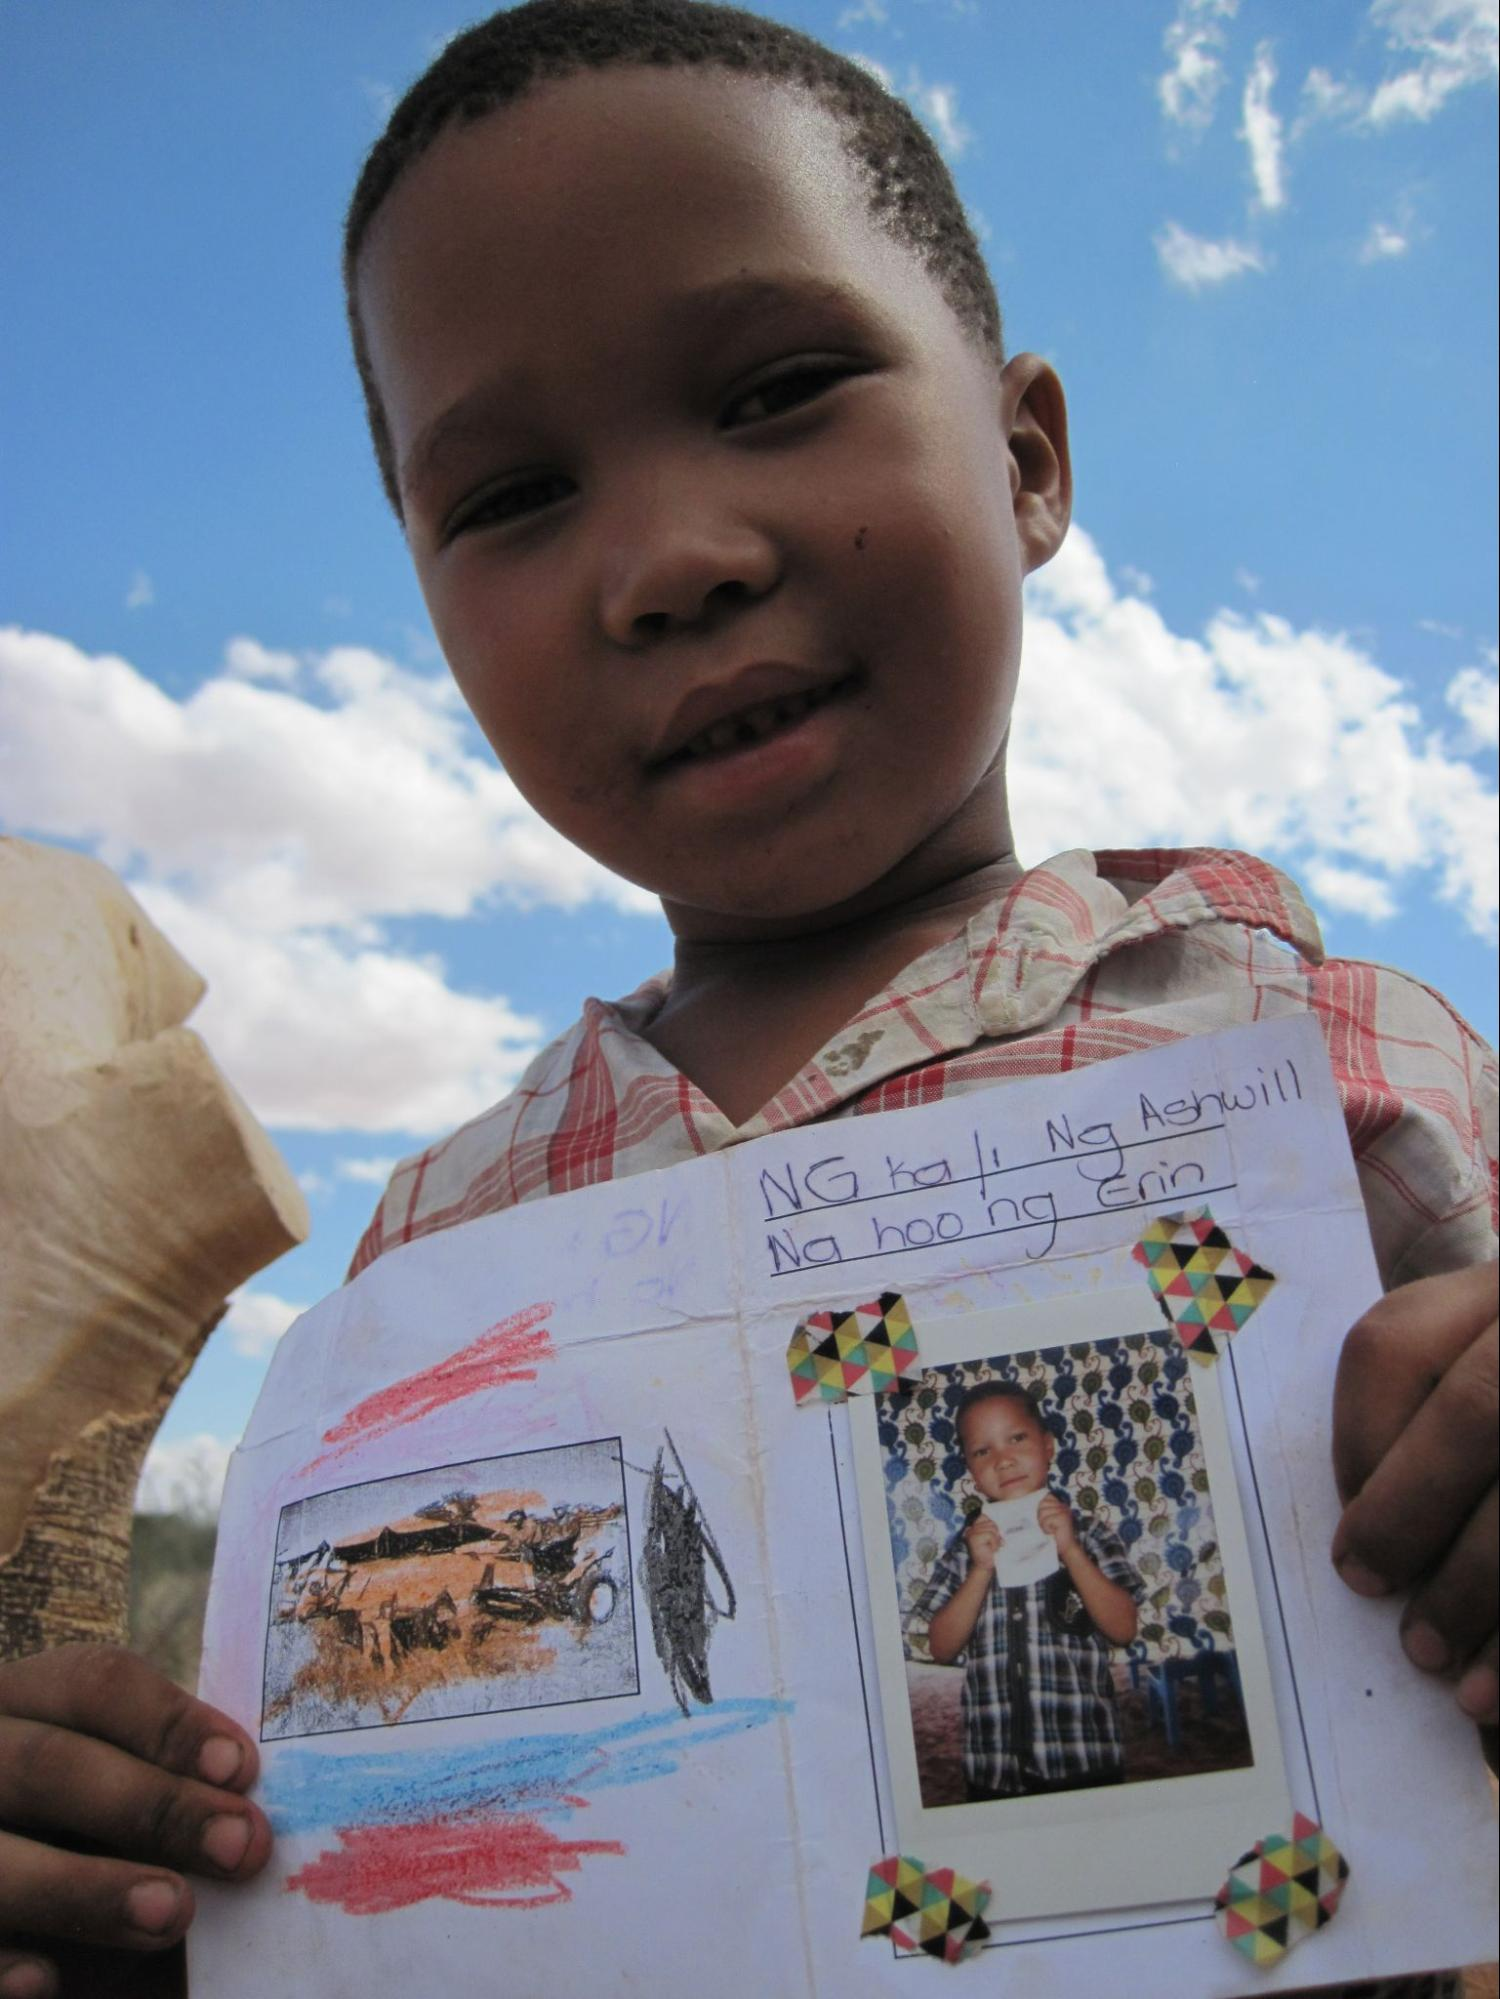
\includegraphics[width=.27\textwidth]{writing.jpg}} \\
        Ouma Katrina leer die kindertjies by haar skool,
        G\textipa{\textdoublebarpipe}aqe
        \textipa{\textdoublevertline}X'oqe
        (Staar na die Sterre), Upington (2015)\footref{kj} &
        Ashwill Raats van Witdraai leer sy eerste geskrewe
        N\textipa{\textvertline}uu-sin by African Tongue se Taaltent,
        Kalahari Desert Festival (2015)\footref{kj}\\

Ouma Katrina teaching the little ones at her school,
    G\textipa{\textdoublebarpipe}aqe
    \textipa{\textdoublevertline}X'oqe (Staar na die Sterre), Upington
        (2015)\footref{kj} &
    Ashwill Raats from Witdraai learning his first written sentences
    in N\textipa{\textvertline}uu with African Tongue, Kalahari Desert
        Festival (2015)\footref{kj}\\
    \end{tabular}\\[1em]

    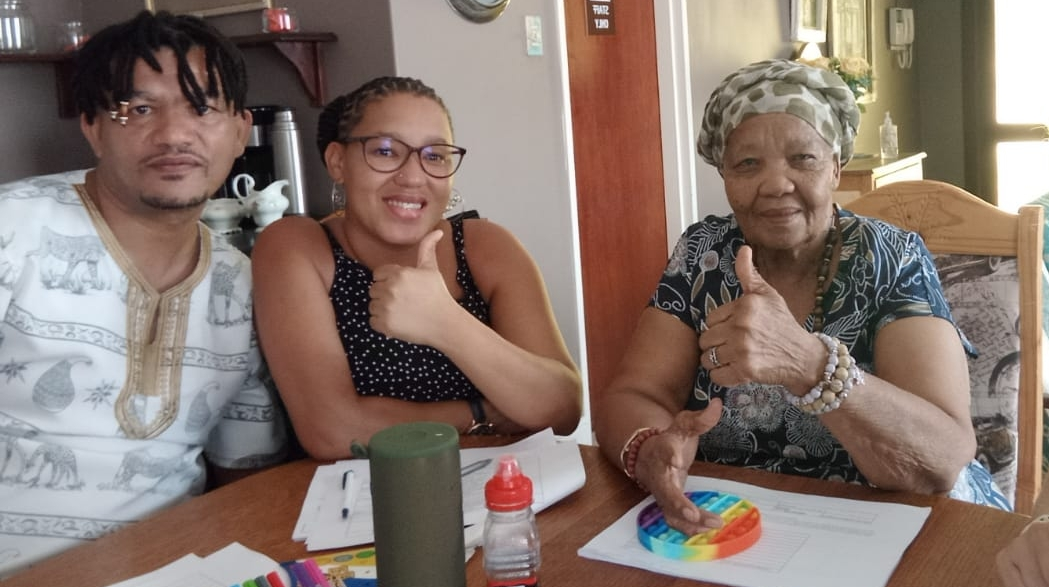
\includegraphics[width=.5\textwidth]{wyk_snyman_esau_crop.jpg}\\
    David van Wyk, Claudia Snyman, Katrina Esau
    (2022)\footref{kj}
\end{center}


\let\Hy@footnote@currentHref\saved@Href@KJ
\addtocounter{footnote}{-1}
\footnotetext{\label{kj}Photo credits: Kerry Jones.}

\let\Hy@footnote@currentHref\saved@Href@LE
\addtocounter{footnote}{1}
\footnotetext{\label{le}Photo credit: Paul Weinberg,
    \textipa{\textdoublebarpipe}Khomani San $|$ Hugh Brody collection,
    University of Cape Town Libraries, Special Collections.}
\makeatother

\newpage

%%%%%%%%%%%%%%%%%%%%%%%%%%%%%%%%%%%%%%%%%%%%%%%%%%%%%%%%%%%%%%%%%%%%%%%%%%%%%%%%

\markboth{}{}
\section{Foto's van bydraers/Photographs of contributors}
\markboth{}{}

\markboth{}{}
\subsection*{N\textipa{\textvertline}uu-sprekers/N\textipa{\textvertline}uu
Speakers\footnote{Photo credits: Antjie Kassie, Griet Seekoei, Hannie
Koerant, Andries Olyn, Hanna Koper, Kheis Brou by Bonny Sands; Vytjie
\textipa{\textvertline}Abaka Koper, GPS\_504-T1-2,
\textipa{\textdoublebarpipe}Khomani San: Hugh Brody collection,
University of Cape Town Libraries, Special Collections;
\textipa{\textvertline}Una Rooi, Film-05\_Frame-21,
\textipa{\textdoublebarpipe}Khomani San: Hugh Brody collection,
University of Cape Town Libraries, Special Collections; Simon Sauls,
by Becky Sands; Elsie Vaalbooi, Kalahari-Archive\_ 0052,
\textipa{\textdoublebarpipe}Khomani San: Hugh Brody collection,
University of Cape Town Libraries, Special Collections.}}
\markboth{}{}

\begin{tabular}{llll}
    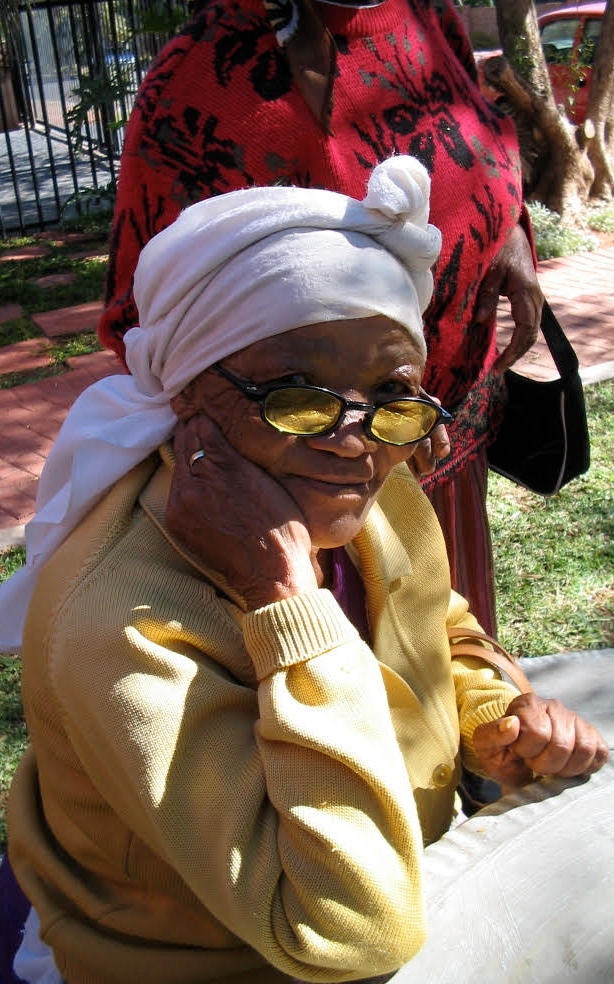
\includegraphics[width=.2\textwidth]{antjie_s.jpg} &
    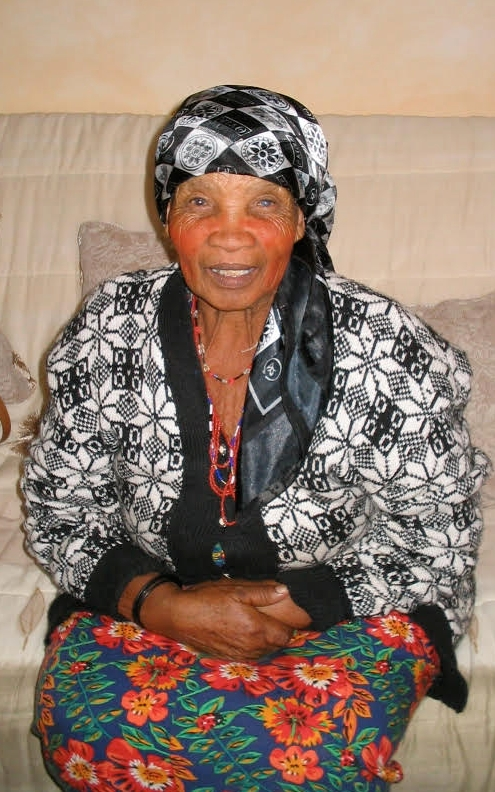
\includegraphics[width=.2\textwidth]{griet_s.jpg} &
    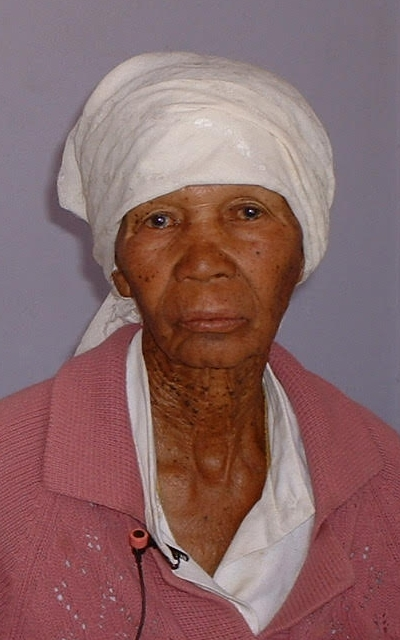
\includegraphics[width=.2\textwidth]{hannie_s.jpg} &
    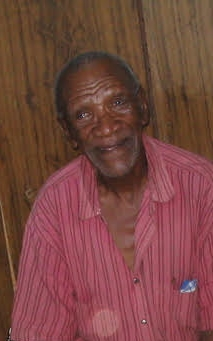
\includegraphics[width=.2\textwidth]{andries_s.jpg} \\
    Antjie Kassie & Griet Seekoei & Hannie Koerant & Andries Olyn \\
    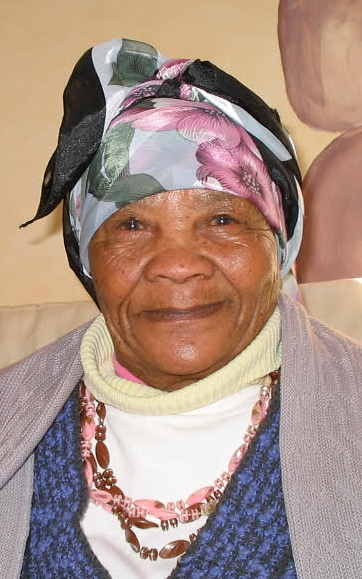
\includegraphics[width=.2\textwidth]{hanna_s.jpg} &
    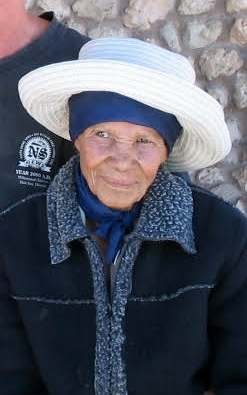
\includegraphics[width=.2\textwidth]{kheis_s.jpg} &
    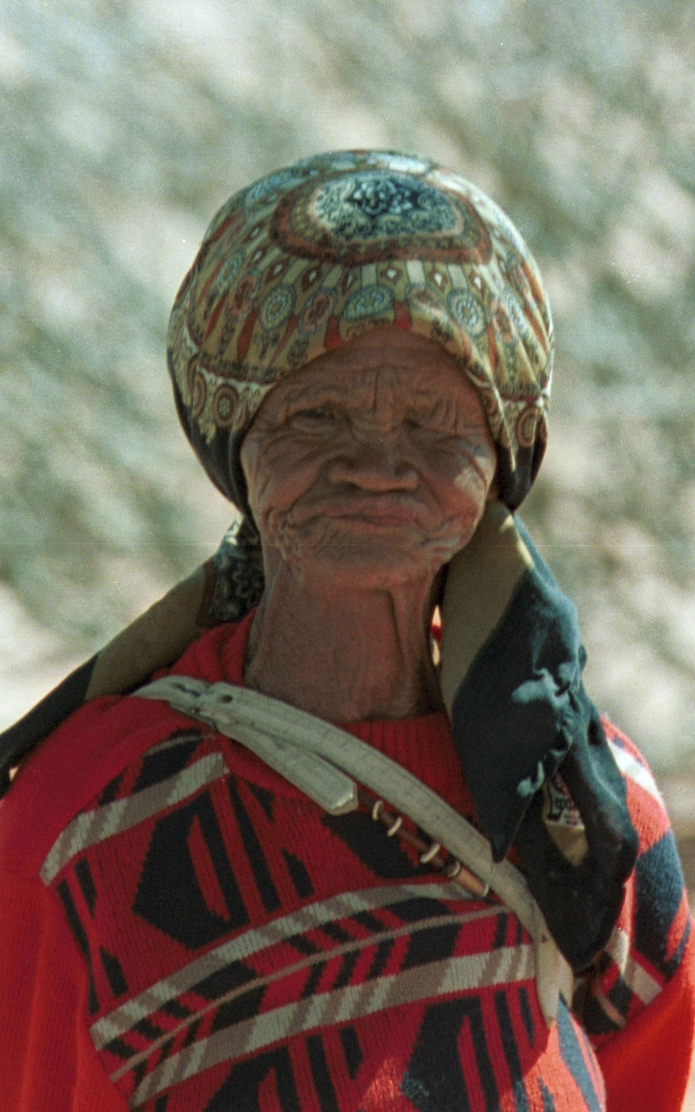
\includegraphics[width=.2\textwidth]{vytjie_s.jpg} &
    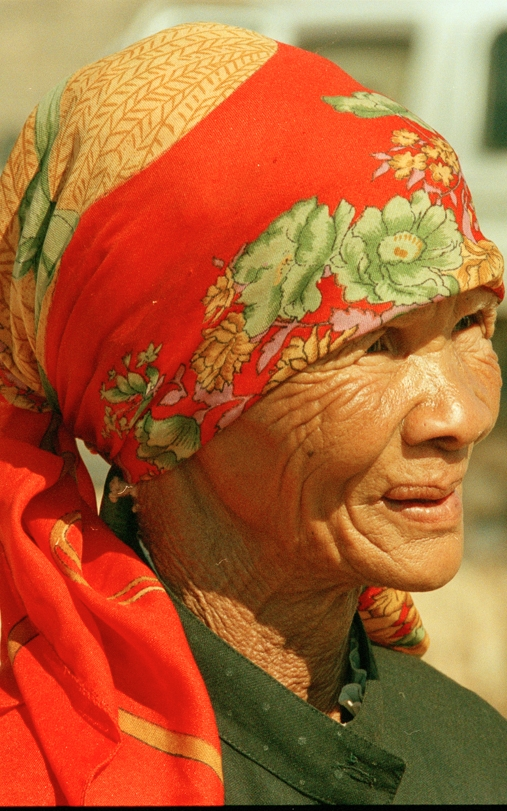
\includegraphics[width=.2\textwidth]{una_s.jpg} \\
    Hanna Koper & Kheis Brou & Vytjie \textipa{\textvertline}Abaka
    Koper & \textipa{\textvertline}Una Rooi \\
    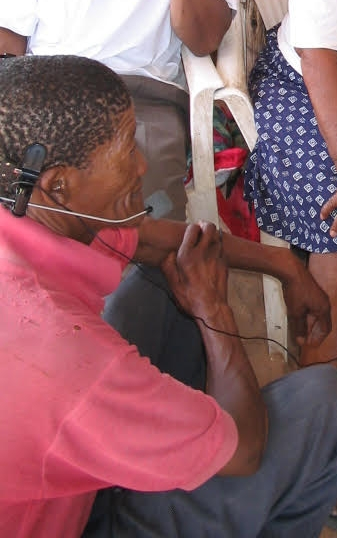
\includegraphics[width=.2\textwidth]{simon_s.jpg} &
    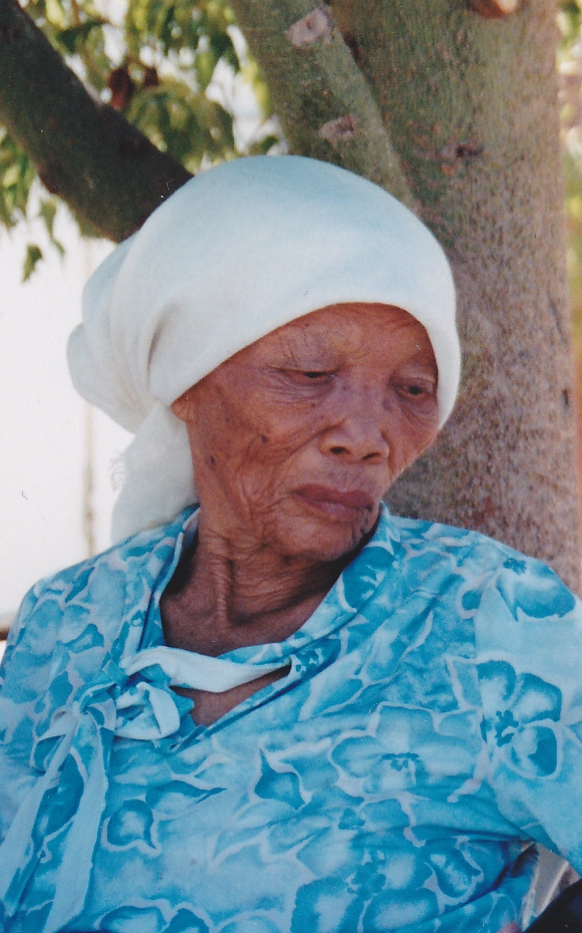
\includegraphics[width=.2\textwidth]{elsie_s.jpg} \\
    Simon Sauls & Elsie Vaalbooi \\
\end{tabular}

\newpage

%%%%%%%%%%%%%%%%%%%%%%%%%%%%%%%%%%%%%%%%%%%%%%%%%%%%%%%%%%%%%%%%%%%%%%%%%%%%%%%%

\markboth{}{}
\subsection*{N\textipa{\textvertline}uu-Taalowerheiddeelnemers/N\textipa{\textvertline}uu
Language Authority Participants\footnote{Photo credits: Katrina Esau
by Kerry Jones; Claudia Snyman by Marshall Coetzee; David van Wyk by
Hugo Bodenham; Mietjie Sussie Bok, photo reproduced with permission.}}
\markboth{}{}

\begin{tabular}{llll}
    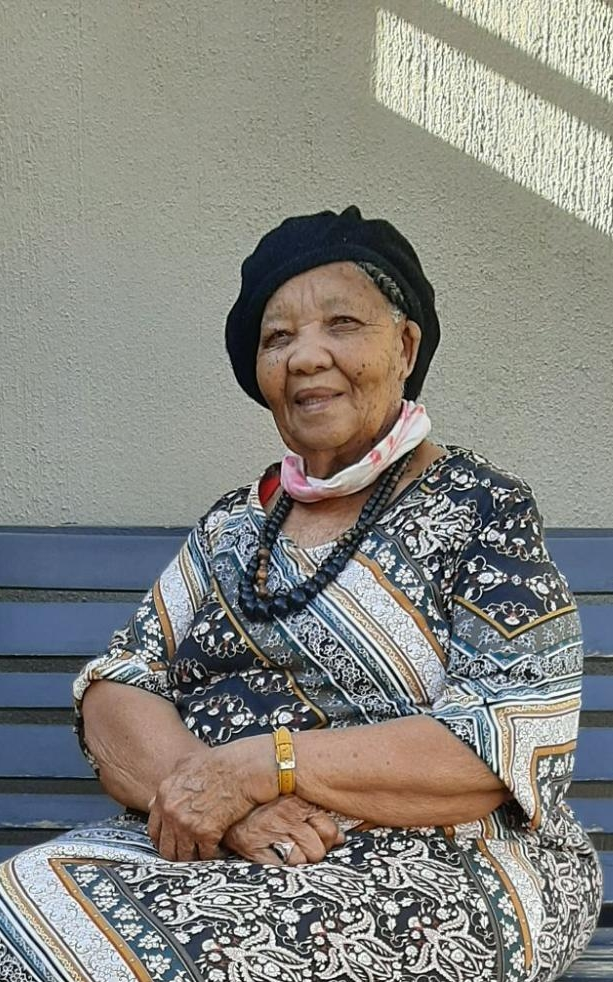
\includegraphics[width=.2\textwidth]{katrina_s.jpg} &
    
\includegraphics[width=.2\textwidth]{claudia_s.jpg} &
    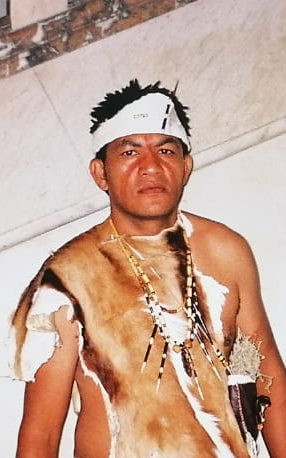
\includegraphics[width=.2\textwidth]{david_s.jpg} &
    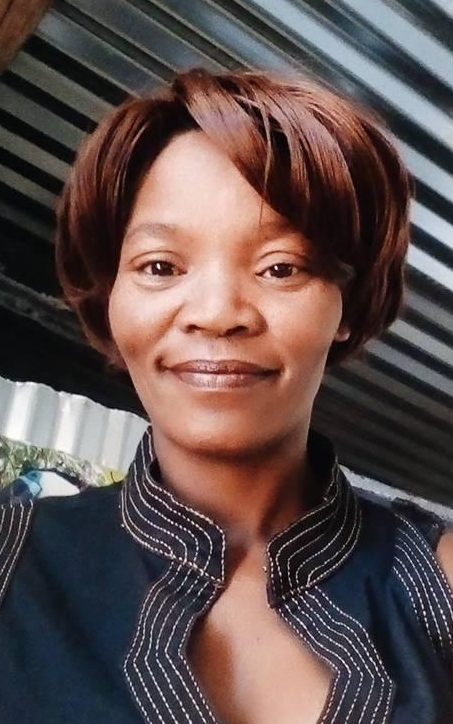
\includegraphics[width=.2\textwidth]{mietjie_s.png} \\
Katrina Esau & Claudia Snyman & David van Wyk & Mietjie Sussie Bok\\
\end{tabular}


\markboth{}{}
\subsection*{Nama-sprekers/Nama Speakers\footnote{Photo credits: Izak
Kruiper by Carl Jones; Lydia Kruiper, Leonard Gewesk, Lys Kruiper
Pietersen by Kerry Jones.}}
\markboth{}{}

\begin{tabular}{llll}
    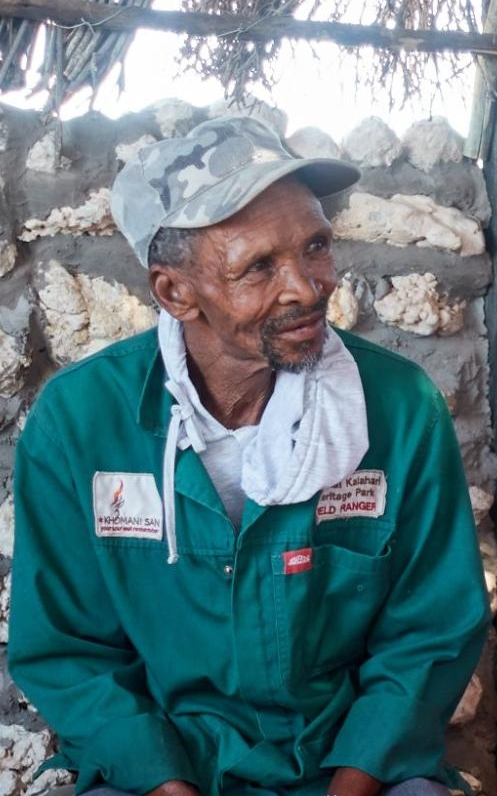
\includegraphics[width=.2\textwidth]{isak_s.jpg} &
    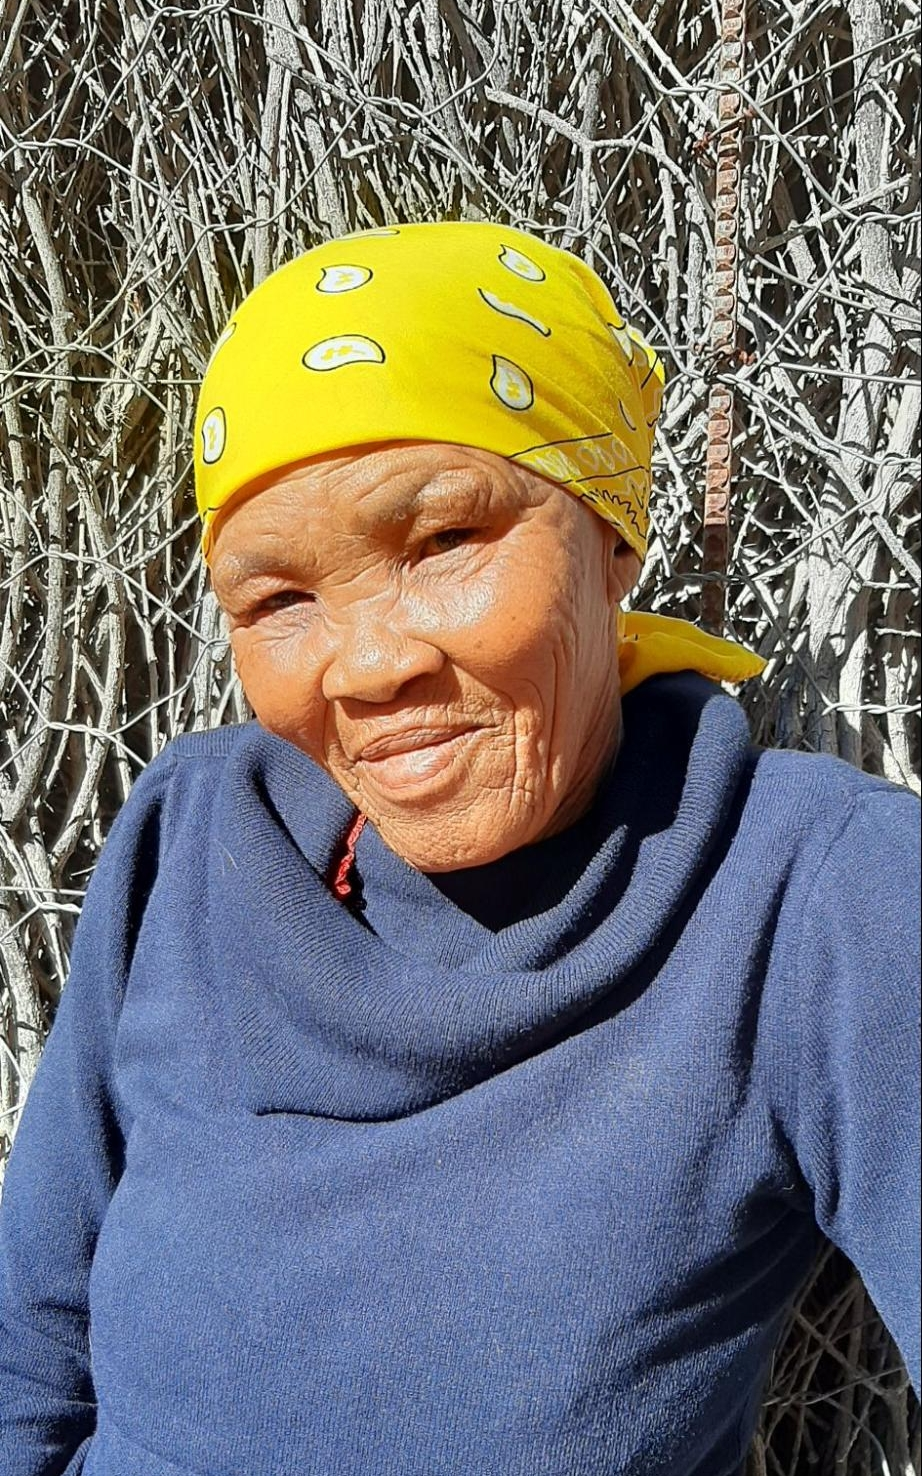
\includegraphics[width=.2\textwidth]{lydia_s.jpg} &
    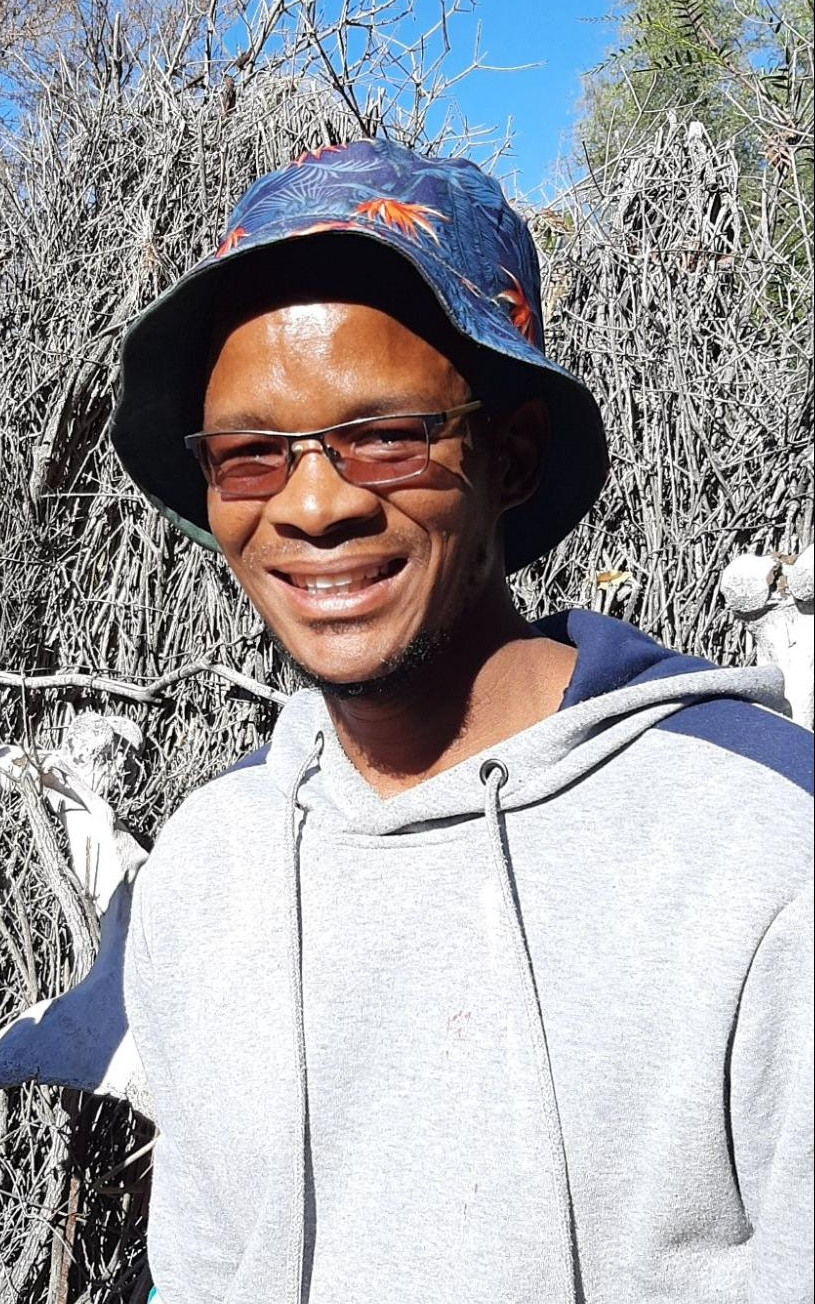
\includegraphics[width=.2\textwidth]{leonard_s.jpg} &
    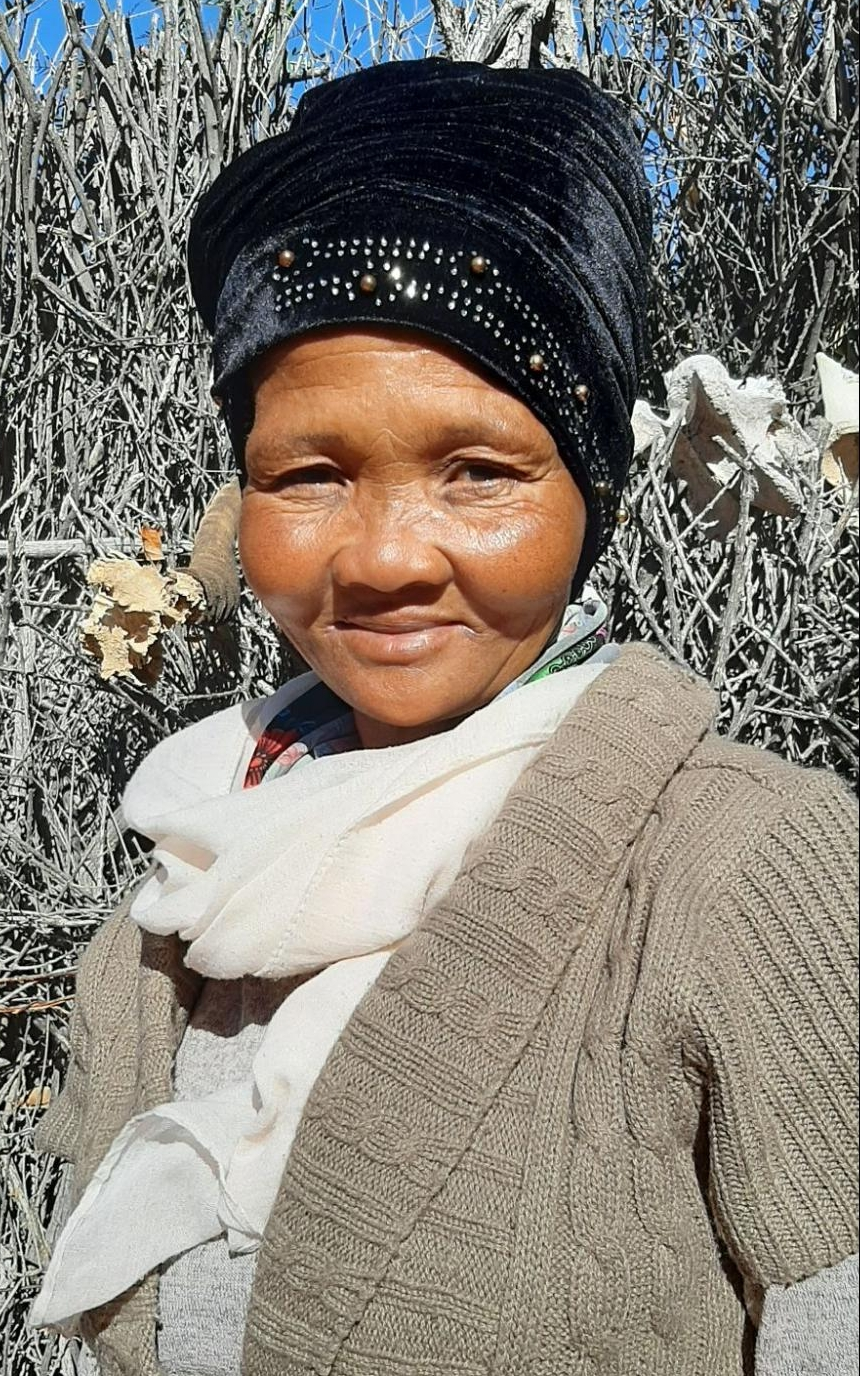
\includegraphics[width=.2\textwidth]{lys_s.jpg} \\
    Izak Kruiper & Lydia (Sakkas) Kruiper & Leonard Gewersk & Lys
    (Oulet) Kruiper Pietersen \\
\end{tabular}


\markboth{}{}
\subsection*{Plaaslike Afrikaanssprekendes/Local Afrikaans
Speakers\footnote{Photo credits: Fritz Jagers, Magdalena James by
Kerry Jones; Hannetjie van der Westhuizen by Johan Nortj\'{e}.}}
\markboth{}{}

\begin{tabular}{lll}
    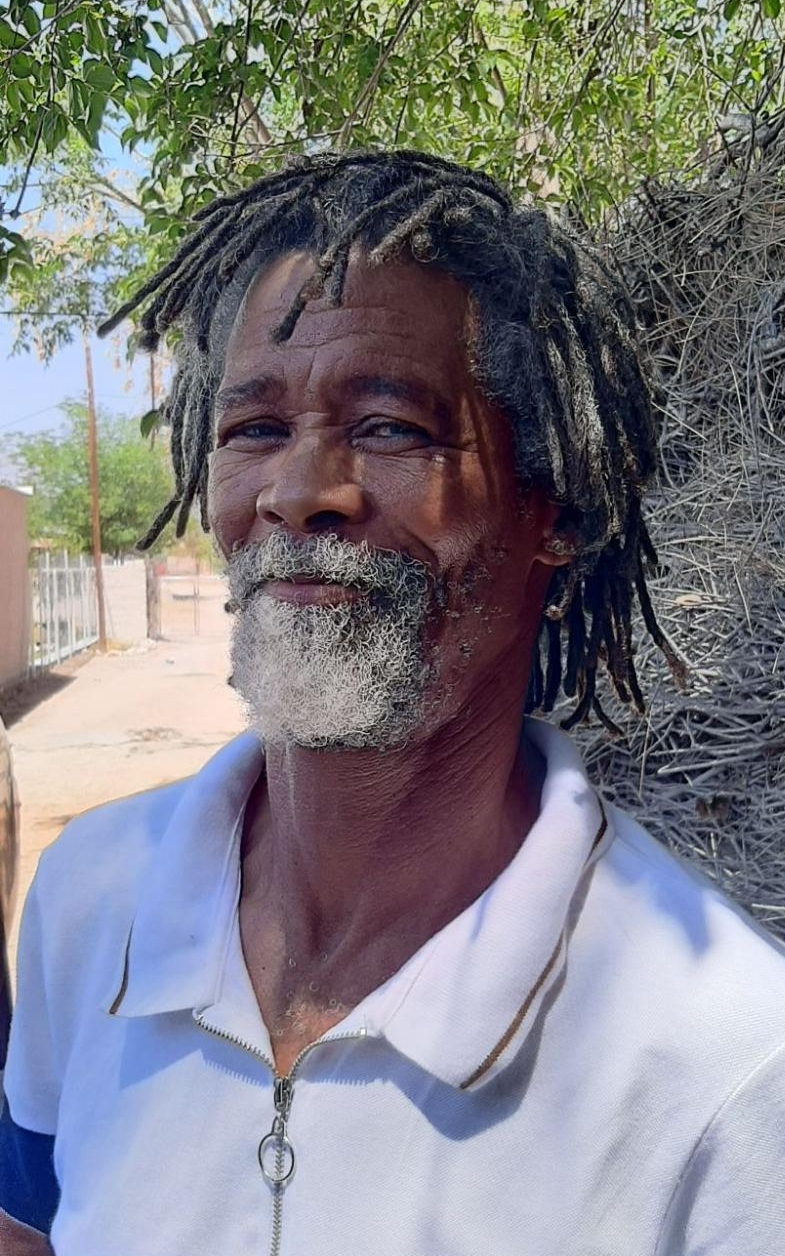
\includegraphics[width=.2\textwidth]{fritz_s.jpg} &
    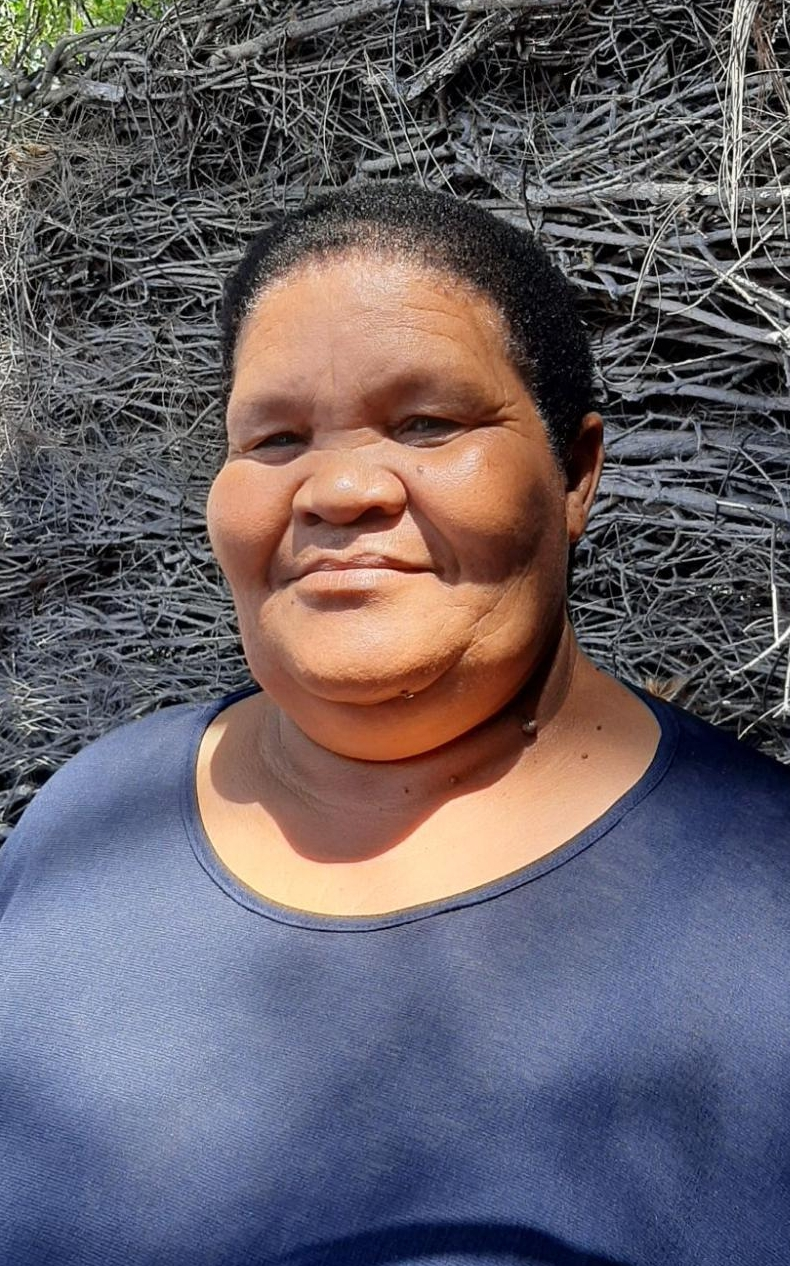
\includegraphics[width=.2\textwidth]{magdalena_s.jpg} &
    
\includegraphics[width=.2\textwidth]{hannetjie_s.jpg} \\
    Fritz Jagers & Magdalena James & Hannetjie van der Westhuizen\\
\end{tabular}

%%%%%%%%%%%%%%%%%%%%%%%%%%%%%%%%%%%%%%%%%%%%%%%%%%%%%%%%%%%%%%%%%%%%%%%%%%%%%%%%

\markboth{}{}
\subsection*{Navorsers en Taalkundiges/Researchers and
Linguists\footnotemark}
%Linguists\footnote{Photo credits: Bonny Sands by Will Grundy; Kerry
%Jones, photo reproduced with permission; Chris Collins by Bonny Sands;
%Alena Witzlack-Makarevich by Bruno Charbit; Sylvanus Job, photo
%reproduced with permission, Francoise (Betta) Steyn by Alexandra
%Labuschagne; Dietloff van der Berg self portrait; Dotty Mantzel by
%Manfred Ceh; Willem Damarah by Kerry Jones; Menno van Zaanen supplied
%by Tilburg University; Amanda Miller, photo reproduced with
%permission; Levi Namaseb, Johanna Brugman by Bonny Sands; Mats Exter,
%photo reproduced with permission.}}
\markboth{}{}

\begin{tabular}{llll}
    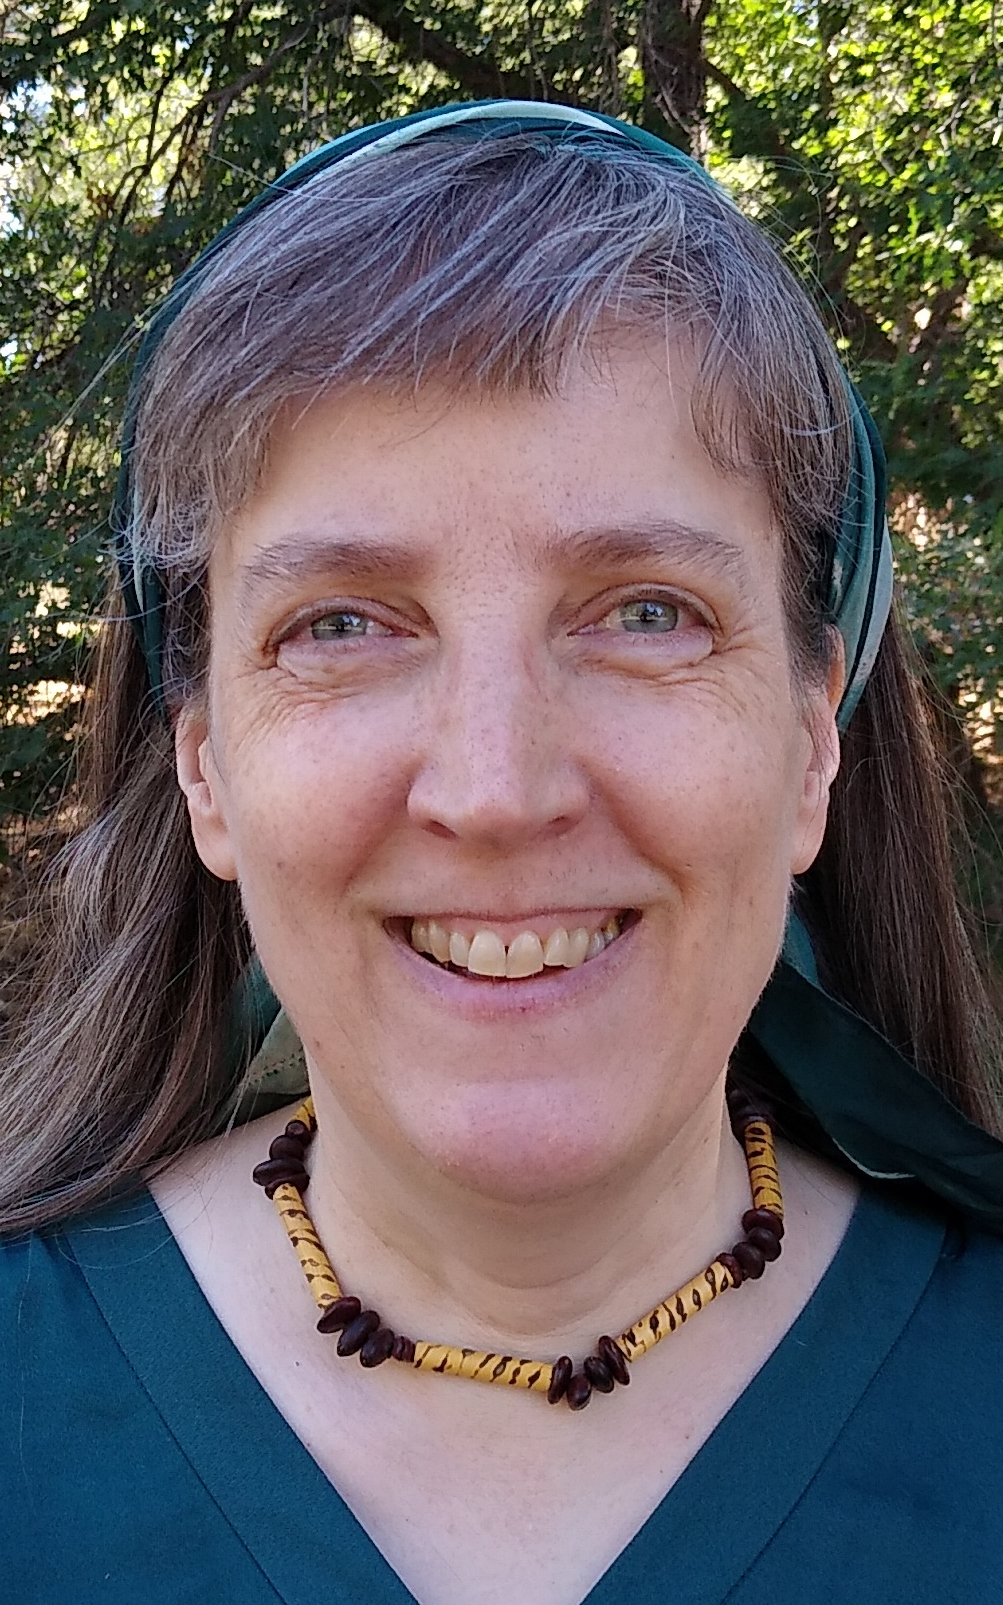
\includegraphics[width=.2\textwidth]{bonny_s.jpg} &
    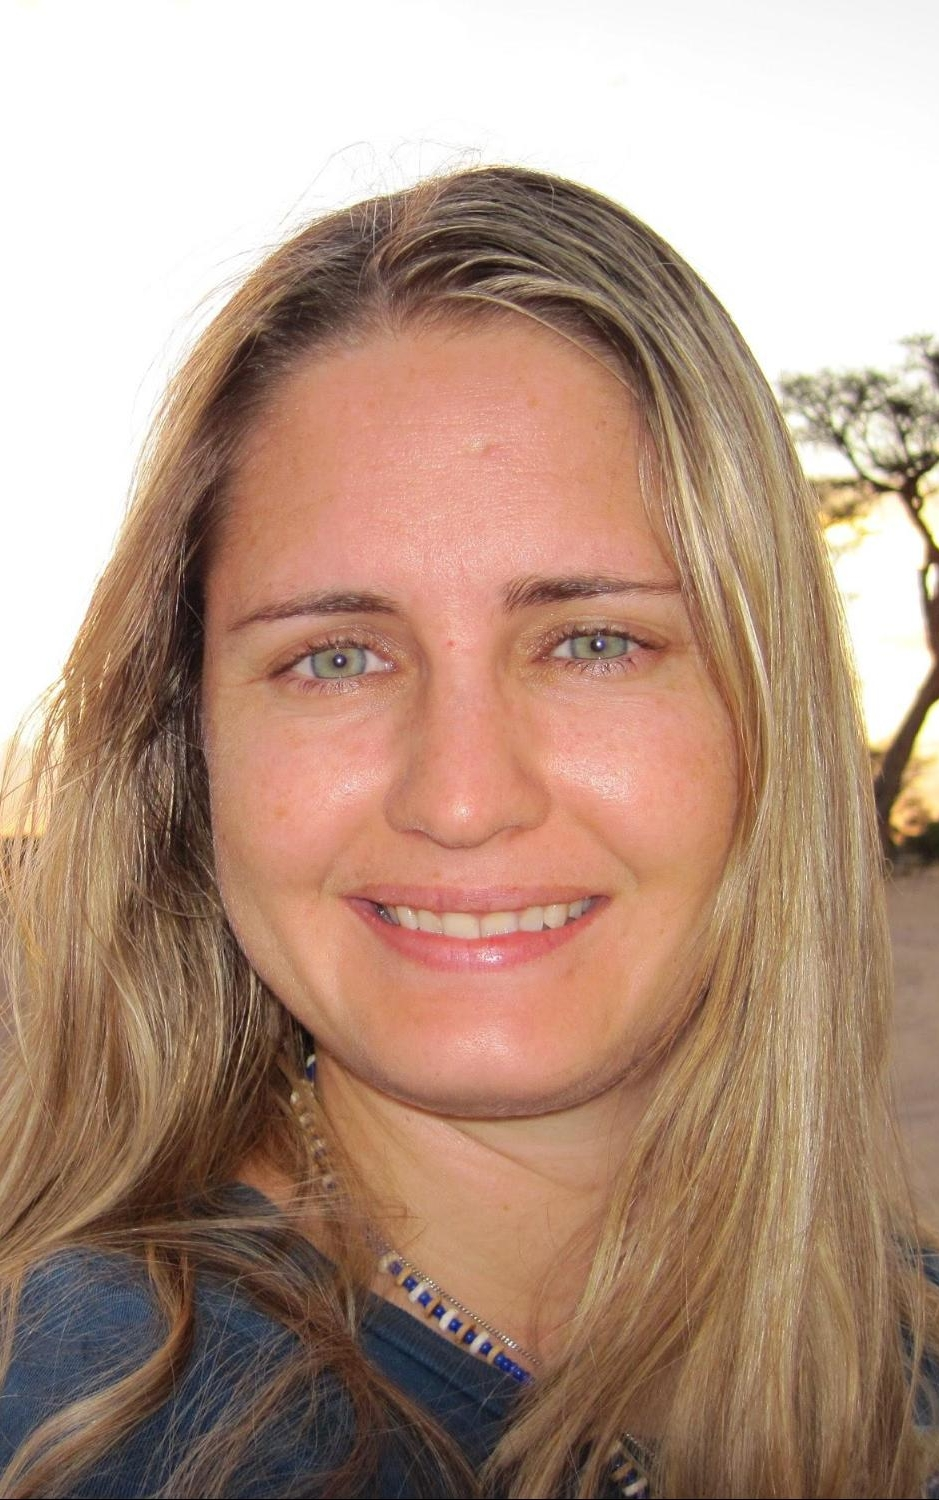
\includegraphics[width=.2\textwidth]{kerry_s.jpg} &
    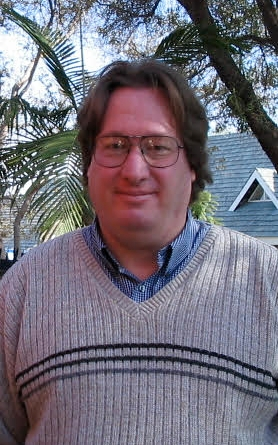
\includegraphics[width=.2\textwidth]{chris_s.jpg} &
    
\includegraphics[width=.2\textwidth]{alena_s.jpg} \\
    Bonny Sands & Kerry Jones & Chris Collins & Alena Witzlack-Makarevich \\
    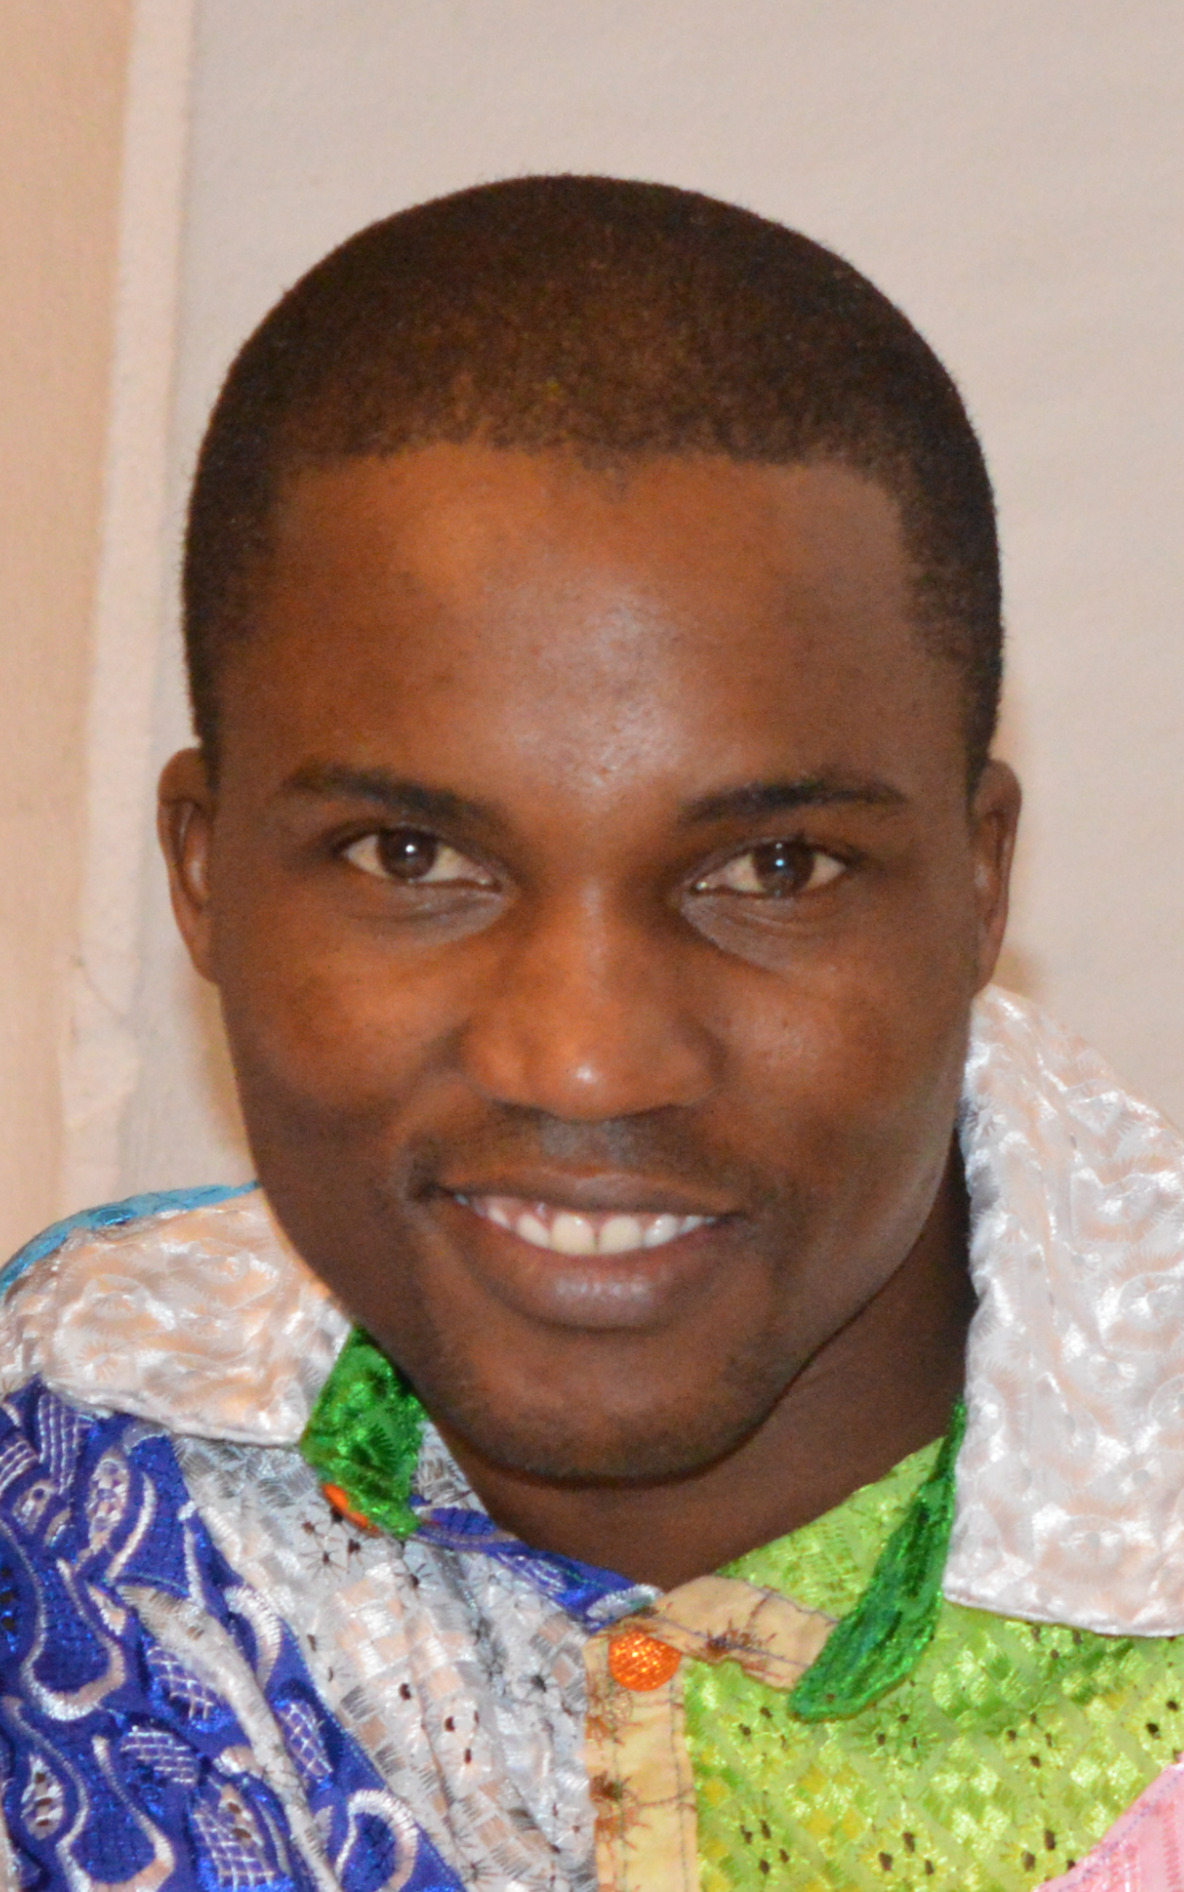
\includegraphics[width=.2\textwidth]{sylvanus_s.png} &
    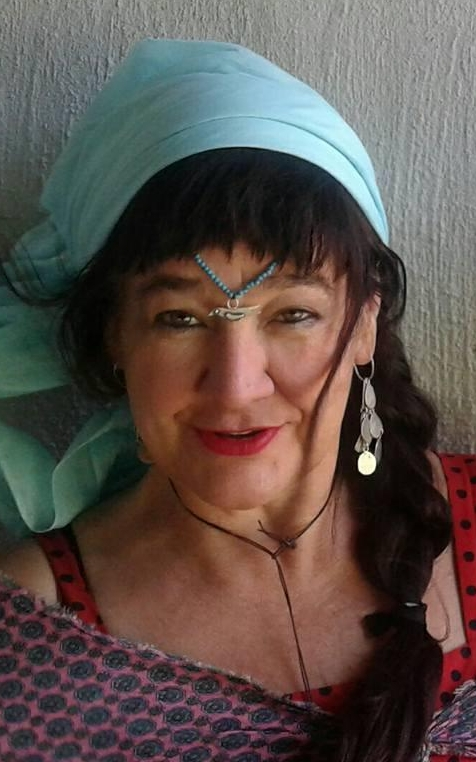
\includegraphics[width=.2\textwidth]{betta_s.jpg} &\
    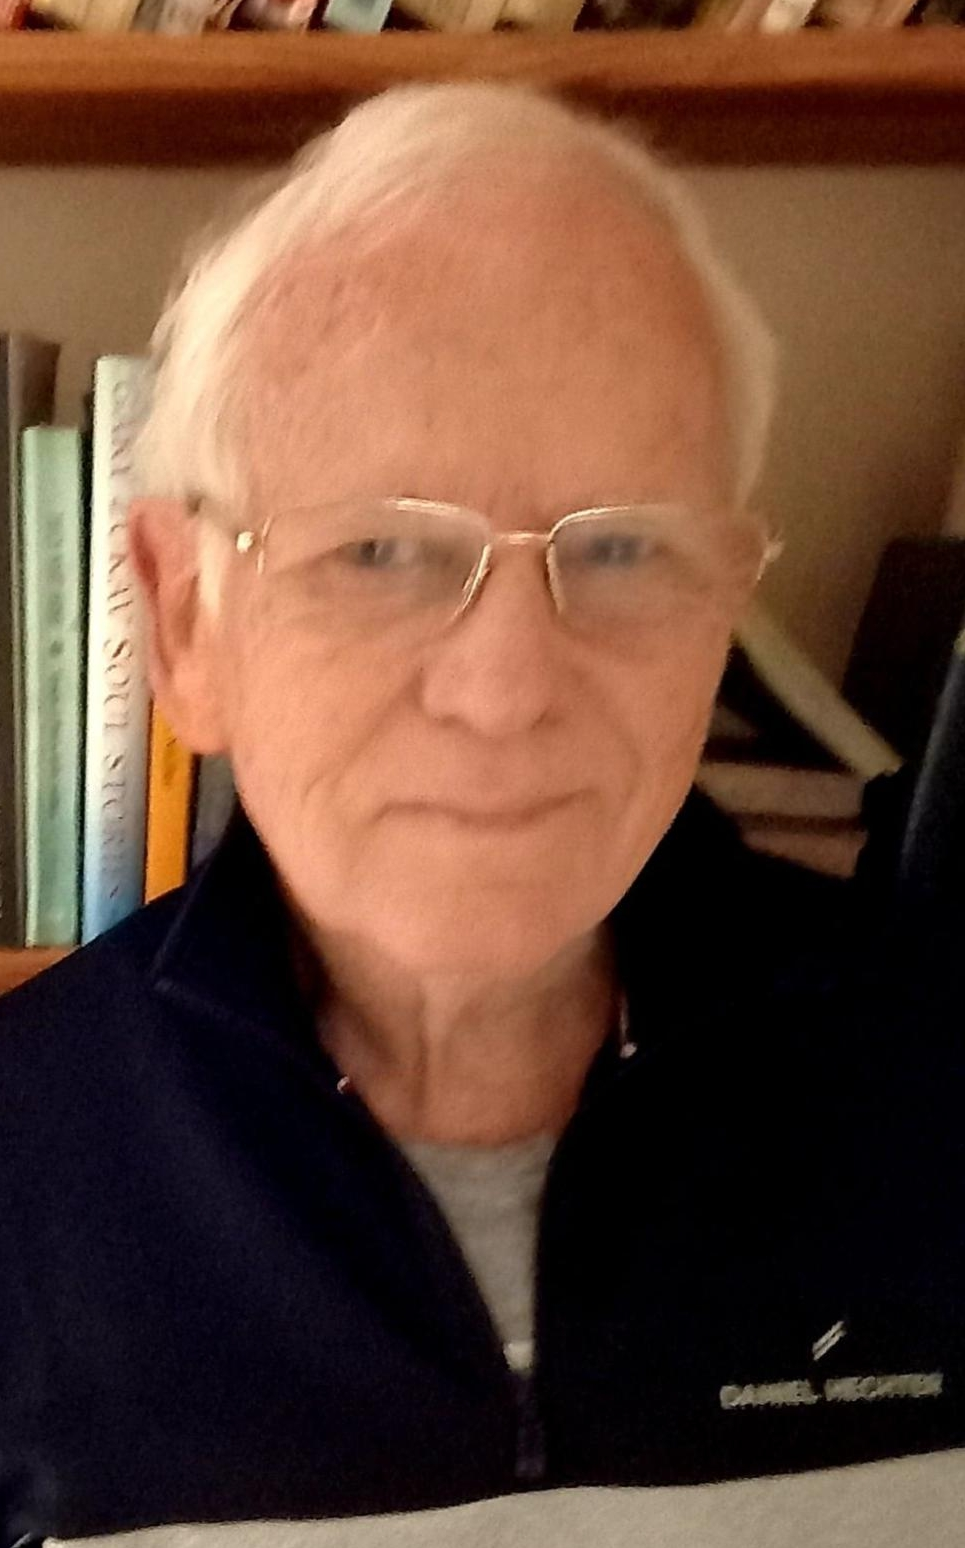
\includegraphics[width=.2\textwidth]{dietloff_s.jpg} &
    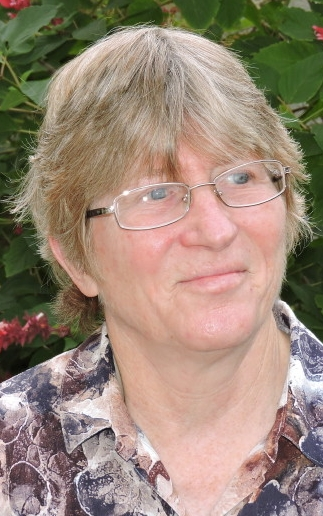
\includegraphics[width=.2\textwidth]{dotty_s.jpg} \\
    Sylvanus Job & Francoise (Betta) Steyn & Dietloff van der Berg &
    Dotty Mantzel \\
    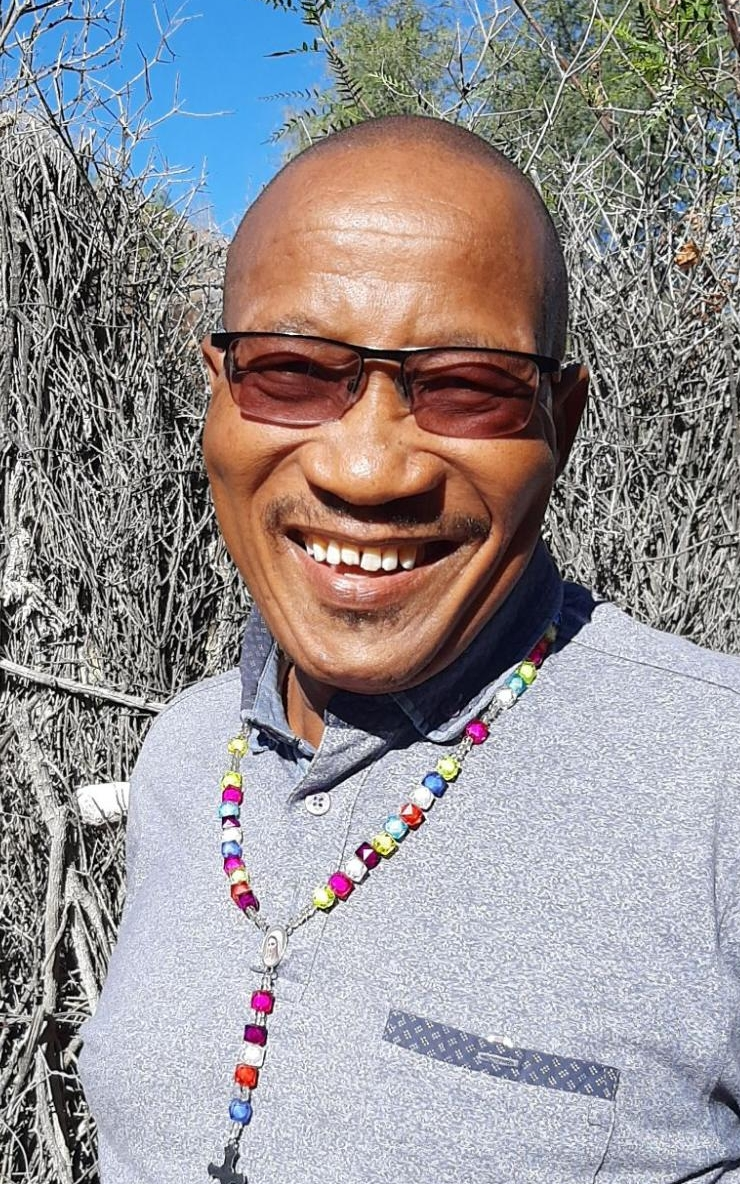
\includegraphics[width=.2\textwidth]{willem_s.jpg} &
    \includegraphics[width=.2\textwidth]{menno_s.jpg} &
    \includegraphics[width=.2\textwidth]{amanda_s.jpg} &
    \includegraphics[width=.2\textwidth]{levi_s.jpg} \\
    Willem Damarah & Menno van Zaanen & Amanda Miller & Levi Namaseb \\
    \includegraphics[width=.2\textwidth]{johanna_s.jpg} &
    \includegraphics[width=.2\textwidth]{mats_s.jpg} &
    \multicolumn{2}{l}{
        \begin{minipage}[b]{.42\textwidth}
\setcounter{mpfootnote}{\thefootnote}
\renewcommand{\thempfootnote}{\arabic{mpfootnote}}
        \footnotetext{Photo credits: Bonny Sands by Will Grundy; Kerry
Jones, photo reproduced with permission; Chris Collins by Bonny Sands;
Alena Witzlack-Makarevich by Bruno Charbit; Sylvanus Job, photo
reproduced with permission, Francoise (Betta) Steyn by Alexandra
Labuschagne; Dietloff van der Berg self portrait; Dotty Mantzel by
Manfred Ceh; Willem Damarah by Kerry Jones; Menno van Zaanen supplied
by Tilburg University; Amanda Miller, photo reproduced with
permission; Levi Namaseb, Johanna Brugman by Bonny Sands; Mats Exter,
photo reproduced with permission.}
    \end{minipage}
}\\
    Johanna Brugman & Mats Exter \\
\end{tabular}


\newpage

%%%%%%%%%%%%%%%%%%%%%%%%%%%%%%%%%%%%%%%%%%%%%%%%%%%%%%%%%%%%%%%%%%%%%%%%%%%%%%%%

\markboth{}{}
\section{Betrokke tale}
\markboth{}{}

Sprekers van N\textipa{\textvertline}uu en ander tale het duisende
jare lank saamgeleef en met mekaar integreer in en om die suidelike
Kalahari-woestyn naby die samevloeiing van die Nossob- en Auobriviere.
Navorsers wat belanggestel het in die mense van hierdie gebied (nou
deel van die Kgalagadi-Oorgrenspark) het in die 1930's die
aanwesigheid van N\textipa{\textvertline}uu opgemerk (wat hulle
\textipa{\textdoublebarpipe}Khomani genoem het), asook tale soos
\textipa{\textvertline}'Auni, \textipa{\textvertline}Haasi
(K'u\textipa{\textvertline}ha\textipa{:}si,
Ki\textipa{\textvertline}hazi), \textipa{\textdoublebarpipe}'Einkusi
(\textipa{\textdoublebarpipe}\~{e}ikusi, Khatia, Kattea, Vaalpens),
Nama en Afrikaans. N\textipa{\textvertline}uu-sprekende oudstes het
ook onthou van die !Ao\textipa{\textdoublebarpipe}ee-mense (Rock
Bushman, Klipboesman) wat eens in die gebied gewoon en 'n eiesoortige
taal gepraat het\footnote{Die taalkundige Anne-Maria Fehn stel voor
dat hulle waarskynlik 'n Khoe-taal van Botswana gepraat het. Hierdie
voorstel is baseer op 'n paar woorde wat Katrina Esau van haar pa se
taal onthou.  Dit stem ooreen met Ouma se verklaring dat haar pa
oorspronklik uit Botswana gekom het.}. Vroe\"{e} navorsers het ook
opgemerk dat Kakia,
N\textipa{\textvertline}u\textipa{\textdoublevertline}en en
N\textipa{\textvertline}amani (N\textipa{\textvertline}amasa) (tale
verwant aan !X\'{o}\~{o} van Botswana) in die suidelike Kalahari naby
die hedendaagse grense van Botswana, Namibi\"{e} en Suid-Afrika
gepraat is. Met die uitsondering van Nama, Afrikaans en
N\textipa{\textvertline}uu, is hierdie tale baie swak gedokumenteer en
word ongelukkig nie meer gepraat nie.\\

N\textipa{\textvertline}uu is eens oor 'n baie wye gebied gepraat. Dit
sluit dele van suidelike Botswana en Namibi\"{e} in en strek vanaf die
sandduine in die noordelikste dele van die Noord-Kaap, suid en
ooswaarts tot in die Langeberg-gebied. Tale soos
\textipa{\textvertline}Xam, !Ora (Korana) en Xri (Griqua, Griekwa) is
ook in aangrensende gebiede gepraat en daar is bewyse dat
N\textipa{\textvertline}uu-sprekendes in die verlede in kontak was met
sprekers van hierdie tale.\\

Onlangs het Kelly Kilian, taalkundige van Rhodes-universiteit
fragmente gedokumenteer van 'n taal wat onthou is deur Elsie George,
Francina George en Robert George, drie sibbe wat in Prieska woon.
Hierdie taal, genaamd Tum\textipa{P}i (Tum'i), is verwant aan sowel
N\textipa{\textvertline}uu as \textipa{\textvertline}Xam, maar
onderskei van elk daarvan \parencite{Kilian2020}. Dit is waarskynlik
dat sprekers van N\textipa{\textvertline}uu in kontak was met sprekers
van Tum\textipa{P}i. Sulke stories herinner ons daaraan dat die
taalkundige voorgeskiedenis van Suid-Afrika beslis meer kompleks is as
wat ons ooit kan weet en dat 'n onverhaalde aantal woorde en tale
vergete is sonder dat dit ooit in geskrewe vorm vasgel\^{e} is.\\

Hierdie woordeboek betrek twee dialekte van die
N\textipa{\textvertline}uu-taal (Oostelik en Westelik), sowel as Nama,
Afrikaans en Suid-Afrikaanse Engels. Di\'{e} woordeboek is nie
eenvoudig vertaal in standaard vari\"{e}teite van Nama en Afrikaans
nie, maar is gebaseer op veldwerk onderneem met sprekers van hierdie
tale in voorheen N\textipa{\textvertline}uu-sprekende gebiede, d.w.s.\
Suid-Afrikaanse Nama en `Onse Afrikaans'. Hierdie tale en dialekte
toon bewyse van die invloed wat hulle mettertyd op mekaar gehad het.\\

Tydens die lees van N\textipa{\textvertline}uu-taalinskrywings mag u
opmerk dat sommige woorde ooreenkomste toon met woorde uit Nama of
Afrikaans. Neemwoorde weerspie\"{e}l 'n geskiedenis van kontak tussen
mense van verskillende talige agtergronde en 'n mate van saamleef waar
verskillende groepe mense mekaar se tale aangeleer het.
N\textipa{\textvertline}uu het woorde oorgeneem uit Afrikaans en Nama,
maar die persentasie woorde wat N\textipa{\textvertline}uu uit hierdie
tale oorgeneem het, is veel minder as die persentasie woorde wat
Engels uit Frans oorgeneem het. Afrikaanssprekendes wat die streek
binnegekom het, het ook woorde oorgeneem uit die tale van die streek
se oorspronklike inwoners. Die plaaslike Afrikaanse woord \emph{!gai}
`wind opbreek' lyk of dit oorgeneem is van of Nama \emph{!gai} of
N\textipa{\textvertline}uu \emph{g!ai}\footnote{Afrikaanssprekers het
baie meer mense wat Nama praat teegekom as mense wat
N\textipa{\textvertline}uu praat. Meeste van die plaaslike kliks in
Afrikaans is dus waarskynlik uit Nama geleen.  Hannie Koerant en
Hannetjie van der Westhuizen vertel egter mondelings van boere wat by
hul Saasi-vriende geleer het om N\textipa{\textvertline}uu te praat.}.
Sommige plaaslike Afrikaanssprekendes spreek die woord uit met 'n
ander klik, \emph{\textipa{\textvertline}gai}. Die plaaslike
Nama-woord \emph{\textipa{\textdoublebarpipe}habe} `man se lendedoek'
lyk of dit oorgeneem is van die Oostelike
N\textipa{\textvertline}uu-woord
\emph{\textipa{\textdoublebarpipe}'haqbe} `man se lendedoek', waardeur
die hardheid van die vokaalklank in die proses wegraak. Ons kan ook
bewyse van die kontak in die plekname van die streek sien. Die
betekenis van die N\textipa{\textvertline}uu-pleknaam \emph{!Ae
Ka\textipa{\textdoublevertline}qhoeke} is byvoorbeeld
`gemsbokhorings'.  Plaaslike Afrikaanssprekendes het die betekenis van
hierdie naam verstaan en na die plek verwys met die naam
\emph{Gemsbokhoring}. Dit is daarna in Engels oorgeneem as
\emph{Gemsbok Horn}.\\

Die N\textipa{\textvertline}uu-plekname in Afdeling~\ref{s:placenames}
lewer moderne bewyse aangaande plekke waar Saasi geleef het en ook
interessante taalfenomene van wedersydse begrip\footnote{Byvoorbeeld
die pan ('n entjie noord van Groot Aar en Klein Aar) wat in
N\textipa{\textvertline}uu as \emph{Ku !Hoe} (let.\ `lyk soos swart')
bekend staan, staan in Afrikaans en Engels as \emph{Swartpan} (let.\
swart pan) bekend. Ons weet nie verseker of hierdie Afrikaanse naam 'n
direkte vertaling van die N\textipa{\textvertline}uu naam is en of dit
onafhanklik na die treffende blink, swart voorkoms van die pan verwys
nie. Die Nama naam \emph{!Noes} (let.\ kol swart dorings) lyk egter of
dit direk deur die N\textipa{\textvertline}uu-naam be\"{\i}nvloed is, met Nama-sprekers wat
'n naam gekies het wat ooreenkom met die uitspraak van die
oorspronklike pleknaam terwyl 'n gedeelte van die oorspronklike naam
behou is.} tussen sprekers van hierdie tale. Eietydse navorsers het in
plekke soos Upington, Olifantshoek, en Andriesvale met Saasi
saamgewerk.\\

\newpage

%%%%%%%%%%%%%%%%%%%%%%%%%%%%%%%%%%%%%%%%%%%%%%%%%%%%%%%%%%%%%%%%%%%%%%%%%%%%%%%%

\markboth{}{}
\addtocounter{section}{-1}
\tocless\section{Featured languages}
\phantomsection
\addcontentsline{toc}{section}{\numberline {\thesection}Featured
languages}
\markboth{}{}

Speakers of N\textipa{\textvertline}uu and other languages have lived
and interacted with one another in and around the southern Kalahari
Desert, near the confluence of the Nossob and Auob Rivers for
thousands of years. Researchers who were interested in the people of
this area (now part of the Kgalagadi Transfrontier Park) in the 1930s,
noted the presence of N\textipa{\textvertline}uu (which they called
\textipa{\textdoublebarpipe}Khomani) as well as languages such as
\textipa{\textvertline}'Auni, \textipa{\textvertline}Haasi
(K'u\textipa{\textvertline}ha\textipa{:}si,
Ki\textipa{\textvertline}hazi), \textipa{\textdoublebarpipe}'Einkusi
(\textipa{\textdoublebarpipe}\~{e}ikusi, Khatia, Kattea, Vaalpens),
Nama and Afrikaans. N\textipa{\textvertline}uu-speaking elders also
recalled the !Ao\textipa{\textdoublebarpipe}ee (Rock Bushman,
Klipboesman) people\footnote{Linguist Anne-Maria Fehn suggests that
they likely spoke a Khoe language of Botswana, based on the few words
that Katrina Esau remembers of her father's language. This accords
with Ouma's statement that her father came from Botswana originally.}
who once lived in the area and spoke a distinct language. Early
researchers also noted that Kakia,
N\textipa{\textvertline}u\textipa{\textdoublevertline}en and
N\textipa{\textvertline}amani (N\textipa{\textvertline}amasa)
(languages related to !X\'{o}\~{o} of Botswana) were spoken in the
southern Kalahari near the modern-day borders of Botswana, Namibia and
South Africa. With the exception of Nama, Afrikaans and
N\textipa{\textvertline}uu, these languages are very poorly documented
and are sadly no longer spoken.\\

N\textipa{\textvertline}uu was once spoken over a very wide area,
including parts of southern Botswana and Namibia, from the sand dunes
in the northernmost parts of the Northern Cape, south and eastward
into the Langberg Mountain area. Languages such as
\textipa{\textvertline}Xam, !Ora (Korana) and Xri (Griqua, Griekwa)
were also spoken in adjacent areas and there is evidence that
N\textipa{\textvertline}uu speakers were in contact with speakers of
these languages in the past.\\

In recent times, linguist Kelly Kilian of Rhodes University documented
fragments of a language remembered by Elsie George, Francina George
and Robert George, three siblings living in Prieska. This language,
called Tum\textipa{P}i (Tum'i), is related to both
N\textipa{\textvertline}uu and \textipa{\textvertline}Xam but distinct
from each of these \parencite{Kilian2020}. It is likely that speakers
of N\textipa{\textvertline}uu were in contact with speakers of
Tum\textipa{P}i. Stories such as this remind us that the linguistic
prehistory of South Africa is certainly more complex than we can ever
know, and that an untold number of words and languages have been
forgotten without ever having been captured in written form.\\

This dictionary features two dialects of the
N\textipa{\textvertline}uu language (Eastern and Western), as well as
Nama, Afrikaans and South African English. This dictionary was not
simply translated into standard varieties of Nama and Afrikaans, but
was based on fieldwork conducted with speakers of these languages
living in previously N\textipa{\textvertline}uu-speaking areas, i.e.\
South African Nama and `Onse Afrikaans'. These languages and dialects
show evidence of their influence on one another over time.\\

In reading N\textipa{\textvertline}uu language entries, you may notice
that some words resemble Nama or Afrikaans words. Loanwords reflect a
history of contact between peoples from different linguistic
backgrounds, and a degree of co-existence where different groups of
people learned one another's languages. N\textipa{\textvertline}uu has
borrowed words from Afrikaans and Nama but the percentage of words
borrowed into N\textipa{\textvertline}uu from these languages is far
lower than the percentage of words in English borrowed from French.
Afrikaans speakers who entered the region also borrowed words from the
languages of the region's original inhabitants. For instance, the
local Afrikaans word \emph{!gai} `belch, burp' appears to be borrowed
from either Nama \emph{!gai} or N\textipa{\textvertline}uu
\emph{g!ai}\footnote{Afrikaans speakers encountered many more people
speaking Nama than N\textipa{\textvertline}uu, so most click words in
local Afrikaans are probably borrowed from Nama. However, there are
oral history accounts from Hannie Koerant and Hannetjie van der
Westhuizen of farmers who learned to speak N\textipa{\textvertline}uu
from their Saasi friends.}. Some local Afrikaans speakers pronounce
the word with a different click, \emph{\textipa{\textvertline}gai}.
The local Nama word \emph{\textipa{\textdoublebarpipe}habe} `man's
loincloth' seems to have been borrowed from the Eastern
N\textipa{\textvertline}uu word
\emph{\textipa{\textdoublebarpipe}'haqbe} `man's loincloth', losing
the harsh quality of the vowel sound in the process. We can also see
evidence of contact in the place names of the region. For example, the
meaning of the N\textipa{\textvertline}uu place name \emph{!Ae
Ka\textipa{\textdoublevertline}qhoeke} is `gemsbok horns'. Local
Afrikaans speakers understood the meaning of this name and referred to
the location with the name \emph{Gemsbokhoring}. This was subsequently
borrowed into English as \emph{Gemsbok Horn}.\\

The N\textipa{\textvertline}uu place names in
Section~\ref{s:placenames} give modern evidence as to locations where
Saasi lived and interesting language contact phenomena of mutual
understanding\footnote{For example, the pan (located a bit north of
Groot Aar and Klein Aar) known in N\textipa{\textvertline}uu as
\emph{Ku !Hoe} (lit.\ `looks like black') is known in Afrikaans and
English as \emph{Swartpan} (lit.\ `black pan'). We can't be certain if
this Afrikaans name was a direct translation of the
N\textipa{\textvertline}uu name or independently bestowed due to the
strikingly shiny black appearance of the pan. However, the Nama name
\emph{!Noes} (lit.\ `patch of black thorns') appears to have been
influenced directly by the N\textipa{\textvertline}uu name, with
Nama-speakers choosing a name that resembled the pronunciation of the
original place name while keeping an aspect of the original meaning
intact.} between speakers of these languages.  Modern-day researchers
worked with Saasi in locations such as Upington, Olifantshoek, and
Andriesvale.\\


\newpage

%%%%%%%%%%%%%%%%%%%%%%%%%%%%%%%%%%%%%%%%%%%%%%%%%%%%%%%%%%%%%%%%%%%%%%%%%%%%%%%%

\markboth{}{}
\section{Hoe om hierdie woordeboek te gebruik/How to use this
dictionary}
\markboth{}{}

In hierdie afdeling bespreek ons/In this section we discuss:
\begin{enumerate}
    \setlength{\itemsep}{-.3em}
    \item[\ref{s:watisin_a}] Wat is in elke woordeboekinskrywing?
    \item[\ref{s:watisin_e}] What is in each dictionary entry?
    \item[\ref{s:pos_a}] Rededeel-etikette
    \item[\ref{s:pos_e}] Part of speech labels
    \item[\ref{s:afk}] Afkortings en akronieme/Abbreviations and acronyms
    \item[\ref{s:lookup_a}] Hoe om 'n woord op te soek
    \item[\ref{s:lookup_e}] How to look up a word
    \item[\ref{s:spelling_a}] Hoe woorde gespel en uitgespreek word
    \item[\ref{s:spelling_e}] How words are spelt\footnote{The choice to
        use `spelt' rather than `spelled' is deliberate. Here and
        throughout the dictionary, we follow South African English
        usage rather than British or American.} and pronounced
    \item [\ref{s:symbols}] Simbole wat in die transkripsie van
        N\textipa{\textvertline}uu-woorde gebruik word/Symbols used in
        the transcription of N\textipa{\textvertline}uu words
\end{enumerate}


\markboth{}{}
\subsection{Wat is in elke woordeboekinskrywing?}
\label{s:watisin_a}
\markboth{}{}

Die volgorde van inligting in elke inskrywing hang af van die afdeling
van die woordeboek. Komponente wat nie ingesluit is in elke inskrywing
nie word hier tussen hakies aangedui. 'n Glos is eenvoudig die basiese
vertaling van 'n woord. Die dialektabel, bv.\ (Oostelik) of
(Westelik), is ingesluit as 'n gelyste vorm wanneer ons weet 'n woord
kom slegs in Oostelike of Westelike N\textipa{\textvertline}uu voor.
Suid-Afrikaanse Nama-vorms is ge\"{e}tiketteer as \underbar{Nama},
Afrikaanse vorms is as \underbar{Afr} ge\"{e}tiketteer, plaaslike
Afrikaanse vorms is as \underbar{Afr$^{\mbox{\footnotesize{ons}}}$}
ge\"{e}tiketteer en Engelse vorms is as \underbar{Eng}
ge\"{e}tiketteer.  Die afkorting NKK dui woorde in Namibiese Khoekhoe
aan waar dit van Suid-Afrikaanse Nama-vorms verskil, of waar die
NKK-vorm bykomende inligting verskaf. Die Internasionale Fonetiese
Alfabet-transkripsie word slegs getoon in die
N\textipa{\textvertline}uu-afdeling van die woordeboek. Ekstra
inligting mag 'n voorbeeldsin of nota oor aanvullende grammatikavorms
van die woord insluit.  Vraagtekens dui aan dat die inligting wat in
die woordeboekinskrywing verskaf word, opsioneel is. 

\begin{description}
    \item [N\textipa{\textvertline}uu-inskrywings:]
        \textbf{N\textipa{\textvertline}uu-woord(e) met opsionele
        dialeketiket(te)}
        (rededeeletiket) [IFA\footnote{Internasionale Fonetiese Alfabet.}
        transkripsie] \underbar{Nama}: Nama-glos (NKK: Namibiese
        Khoe\-khoe-vorm)$^?$ \underbar{Afr}: Afrikaanse
        glos \underbar{Afr$^{\mbox{\footnotesize{ons}}}$}: plaaslike
        Afrikaanse glos$^?$ \underbar{Eng}: Engelse glos
        \underbar{\textit{Nama}}: ekstra inligting in Nama$^?$
        \underbar{\textit{Afr}}: ekstra inligting in Afrikaans$^?$
        \underbar{\textit{Eng}}: ekstra inligting in Engels$^?$
    \item [Nama-inskrywings:] \textbf{Nama-glos} (NKK: Namibiese
        Khoekhoe-vorm)$^?$ (rededeeletiket)
        \underbar{N\textipa{\textvertline}uu}:
        N\textipa{\textvertline}uu-woord(e) met opsionele
        dialeketiket(te) \underbar{Afr:} Afrikaanse
        glos \underbar{Afr$^{\mbox{\footnotesize{ons}}}$}: plaaslike
        Afrikaanse glos$^?$ \underbar{Eng}: Engelse glos
        \underbar{\textit{Nama}}: ekstra inligting in Nama$^?$
        \underbar{\textit{Afr}}: ekstra inligting in Afrikaans$^?$
        \underbar{\textit{Eng}}: ekstra inligting in Engels$^?$
    \item [Afrikaanse inskrywings:] \textbf{Afrikaanse glos}
        \underbar{Afr$^{\mbox{\footnotesize{ons}}}$}: plaaslike
        Afrikaanse glos$^?$ (rededeeletiket)
        \underbar{N\textipa{\textvertline}uu}:
        N\textipa{\textvertline}uu-woord(e) met opsionele
        rededeeletiket(te) \underbar{Nama}: Nama-glos 
        (NKK: Namibiese Khoekhoe-vorm)$^?$ \underbar{Eng}: Engelse
        glos \underbar{\textit{Afr}}: ekstra inligting in
        Afrikaans$^?$ \underbar{\textit{Nama}}: ekstra inligting in
        Nama$^?$ \underbar{\textit{Eng}}: ekstra inligting in
        Engels$^?$
    \item [Engelse inskrywings:] \textbf{Engelse glos}
        (rededeeletiket) \underbar{N\textipa{\textvertline}uu}: N\textipa{\textvertline}uu-woord(e) met
        opsionele dialeketiket(te) \underbar{Nama}: Nama-glos (NKK:
        Namibiese Khoe\-khoe-vorm)$^?$
        \underbar{Afr}: Afrikaanse glos
        \underbar{Afr$^{\mbox{\footnotesize{ons}}}$}: plaaslike
        Afrikaanse glos$^?$ \underbar{\textit{Eng}}: ekstra
        inligting in Engels$^?$ \underbar{\textit{Nama}}: ekstra
        inligting in Nama$^?$ \underbar{\textit{Afr}}: ekstra
        inligting in Afrikaans$^?$
\end{description}


\markboth{}{}
\addtocounter{subsection}{-1}
\tocless\subsection{What is in each dictionary entry?}
\phantomsection
\addcontentsline{toc}{subsection}{\numberline {\thesubsection}What is
in each dictionary entry?}
\label{s:watisin_e}
\markboth{}{}

The order of information in each entry depends on the section of the
dictionary. Components that are not included in every entry are listed
here in parentheses. A gloss is simply the basic translation of a
word. The dialect label, e.g.\ (Eastern) or (Western), is included if
a form listed is known to only occur in either Eastern or Western
N\textipa{\textvertline}uu. South African Nama forms are labelled
\underbar{Nama}, Afrikaans forms are labelled \underbar{Afr}, local
Afrikaans forms are labelled
\underbar{Afr$^{\mbox{\footnotesize{ons}}}$} and English forms are
labelled \underbar{Eng}. The abbreviation NKK indicates words in
Namibian Khoekhoe where these differ from the South African Nama
forms, or where the NKK form provides additional information. The
International Phonetic Alphabet transcription is only shown in the
N\textipa{\textvertline}uu section of the dictionary. Extra
information may include an example sentence or note about additional
grammatical forms of the word.  Question marks indicate that the
provided information is optional in the dictionary entry. 

\begin{description}
    \item [N\textipa{\textvertline}uu entries:]
        \textbf{N\textipa{\textvertline}uu word(s) with optional
        dialect label(s)} (part of
        speech label) [IPA\footnote{International Phonetic Alphabet.}
        transcription] \underbar{Nama}: Nama gloss (NKK: Namibian
        Khoekhoe form)$^?$ \underbar{Afr}: Afrikaans
        gloss \underbar{Afr$^{\mbox{\footnotesize{ons}}}$}: local
        Afrikaans gloss$^?$ \underbar{Eng:} English gloss
        \underbar{\textit{Nama}}: extra
        information in Nama$^?$ \underbar{\textit{Afr}}: extra
        information in Afrikaans$^?$ \underbar{\textit{Eng}}: extra
        information in English$^?$
    \item [Nama entries:] \textbf{Nama gloss} (NKK: Namibian Khoekhoe
        form)$^?$ (part
        of speech label) \underbar{N\textipa{\textvertline}uu}:
        N\textipa{\textvertline}uu word(s) with optional dialect
        label(s) \underbar{Afr}: Afrikaans gloss
        \underbar{Afr$^{\mbox{\footnotesize{ons}}}$}: local Afrikaans
        gloss$^?$ \underbar{Eng}: English gloss
        \underbar{\textit{Nama}}: extra information in Nama$^?$
        \underbar{\textit{Afr}}: extra information in
        Afrikaans$^?$ \underbar{\textit{Eng}}: extra information in
        English$^?$
    \item [Afrikaans entries:] \textbf{Afrikaans gloss}
        \underbar{Afr$^{\mbox{\footnotesize{ons}}}$}: local Afrikaans
        gloss$^?$ (part of speech label)
        \underbar{N\textipa{\textvertline}uu}:
        N\textipa{\textvertline}uu word(s) with optional dialect
        label(s) \underbar{Nama}: Nama gloss (NKK: Namibian Khoekhoe
        form)$^?$ \underbar{Eng}: English
        gloss \underbar{\textit{Afr}}: extra information in
        Afrikaans$^?$ \underbar{\textit{Nama}}: extra information in
        Nama$^?$ \underbar{\textit{Eng}}: extra information in
        English$^?$
    \item [English entries:] \textbf{English gloss} (part of speech
        label) \underbar{N\textipa{\textvertline}uu}: 
        N\textipa{\textvertline}uu word(s) with optional dialect
        label(s) \underbar{Nama}: Nama gloss
        (NKK: Namibian Khoekhoe form) \underbar{Afr}: Afrikaans gloss
        \underbar{Afr$^{\mbox{\footnotesize{ons}}}$}: local Afrikaans
        gloss$^?$ \underbar{\textit{Eng}}: extra information in
        English$^?$ \underbar{\textit{Nama}}: extra information in
        Nama$^?$ \underbar{\textit{Afr}}: extra information in
        Afrikaans$^?$
\end{description}



\markboth{}{}
\subsection{Rededeel-etikette}
\label{s:pos_a}
\markboth{}{}

Die rededeeletiket dui aan hoe die N\textipa{\textvertline}uu-woord of
inskrywing in 'n sin werk. Die mees algemene soort inskrywing (T1) is
'n naamwoord. Die soort woorde wat naamwoorde is, is di\'{e} wat
verwys na fisieke voorwerpe, stowwe, mense, plante, diere, en
liggaamsdele. Voorbeelde van naamwoorde sluit in: \emph{!uuke} `skoen'
\emph{!qhaa} `water', \emph{\textipa{\textdoublevertline}aaxe}
`suster', \emph{\textipa{\textdoublebarpipe}ausi} `tsamma',
\emph{\textipa{\textdoublevertline}xuri} `wildehond',
\emph{n\textipa{\textvertline}um} `baard', ens.  Naamwoorde kan ook
toestande of aktiwiteite soos \emph{k\^{o}eaki} `geluk' of
\emph{\textipa{\textvertline}x'\^{o}aki} `jag' wees. Eiename (T1b)
word nie in die woordeboek aangegee nie, maar word egter onder hierdie
inleiding aangegee. Eiename sluit die name van mense en plekke in.
Naamwoordsamestellings, of naamwoorde wat uit twee naamwoorde bestaan,
word as een woord geskryf, bv.\
\emph{ts'uruke\textipa{\textvertline}qhuisi} `muisvo\"{e}l'
(saamgestel uit \emph{ts'uruke} `muis' en
\emph{\textipa{\textvertline}qhuisi} `vo\"{e}l'),
\emph{ts'axam\textipa{\textvertline}huuke} `ooghare' (saamgestel uit
\emph{ts'axam} `oog' en \emph{\textipa{\textvertline}huuke} `hare').\\

Die tweede mees algemene soort inskrywing (T2) is 'n werkwoord.
Werkwoorde druk gewoonlik aktiwiteite of handelinge soos \emph{!ai}
`hardloop', \emph{\textipa{\textvertline}x'\^{o}a} `jag',
\emph{!'h\^{o}e} `vra', en \emph{g!ara} `l\^{e} op jou rug' uit.
Werkwoorde vorm die kern van sinne en dra wat gebeur of wat gedoen
word, oor. Baie woorde wat toestande of handelingswyses uitdruk, soos
\emph{\textipa{\textdoublevertline}'huu} `opgewonde wees',
\emph{\textipa{\!o}'ui'i} `siek wees' en
\emph{\textipa{\textdoublevertline}'um'i} `swaar wees' is ook
werkwoorde in N\textipa{\textvertline}uu. Dit wil s\^{e} dit kom voor
in sinne sonder 'n \emph{wees}-werkwoord - anders as in Afrikaans en Engels.
N\textipa{\textvertline}uu het baie werkwoordsamestellings (T2) wat
bestaan uit meer as een werkwoord, soos
\emph{\textipa{\textvertline}i!oo} `vat en sit neer' (bestaande uit
\emph{\textipa{\textvertline}i} `vat' en \emph{!oo} `sit') en
\emph{\textipa{\textdoublevertline}'aan!uu} `gaan besoek' (bestaande
uit \emph{\textipa{\textdoublevertline}'aa} `gaan' en \emph{n!uu}
`besoek'). Daar is ook gevalle waar 'n werkwoord en 'n naamwoord 'n
saamgestelde werkwoord vorm (T2), bv.\ \emph{s\^{u}in!\^{o}ake} `sit
gehurk op jou hakke' (bestaande uit \emph{s\^{u}i} `sit' en
\emph{n!\^{o}ake} `hakke').\\

Daar is baie kort woordjies wat belangrike boustene in
N\textipa{\textvertline}uu-grammatika vorm. Voornaamwoorde (T4) is
kort \mbox{woordjies} wat die plek van ander naamwoorde inneem. Die
betekenis van \emph{na} `ek' verander byvoorbeeld afhangend van wie
praat.  Woorde wat na dinge soos \emph{a} `hierdie' verwys, is ook
voornaamwoorde want dit verwys na verskillende dinge afhangend van
waarna verwys of waarna gewys word. Vraende voornaamwoorde soos
\emph{je?} `waar?', help om vrae te vorm. Partikels of deelwoorde (T3)
sluit al die ander boustene in wat nie ingedeel word in een van die
kategorie\"{e} wat in hierdie afdeling beskryf is nie. Voorbeelde van
deelwoorde is \emph{\textipa{\textdoublevertline}u} `nie',
\emph{n\textipa{\textvertline}a} `en, met', en \emph{!'u} `weg'.\\

Sommige frases (T5) tree as sinne op. Voorbeelde hiervan is
\emph{Aio.}\ `Dankie.', en \emph{\textipa{\textdoublebarpipe}'An'a!}\
`Pasop!' in. Frases is gewoonlik sinstukke of woordgroepe. Sommige
frases tree as naamwoorde op.  Voorbeelde van naamwoordfrases (T1a) is
\emph{N\textipa{\textvertline}uu
\textipa{\textdoublebarpipe}xoaki\textipa{\textdoublebarpipe}xanisi}
`N\textipa{\textvertline}uu-taalboek', \emph{n!\^{a}u ke cxaa} `sonop'
(let.\ `wanneer die haas skeur/afskeur'), en
\emph{\textipa{\textdoublevertline}xauke ni jaqn} (Westelik),
\emph{\textipa{\textdoublevertline}hauke hin dj\^{a}qi} (Oostelik)
`vloeiende bloed (nie uit die neus nie)', let.\ `bloed wat loop'.
Sommige frases tree as werkwoorde op. Voorbeelde van werkwoordfrases
(T2a) is \emph{kx'am kq\^{o}e} `wees beter' (lit.\ `waar' + `wees
goed'), \emph{n\textipa{\textvertline}aa
\textipa{\textdoublevertline}'\^{u}i} `word gebore' (let.\ `sien die
son'), en \emph{kx'u kx'amki \textipa{\!o}un} `slaap diep', en
\emph{kx'u kan!\^{u}u \textipa{\!o}one} `wees soos duintjies, wees
effens deinend'.\\

Telwoorde (T8) dui 'n getal aan, bv.\ \emph{!'uu} `twee' terwyl
kwantifiseerders (T11) die hoeveelheid aandui, bv.\ \emph{huniki}
`almal', \emph{\textipa{\textdoublevertline}'ooke} `slegs'.
Tussenwerpsels (T9) soos \emph{ee} `ja', en \emph{n!oo'i} `nee' is
ekspressiewe woorde wat effens anders as naamwoorde en werkwoorde en
meer soos klein sinnetjies is.\\

Byvoeglike naamwoorde (T10) is woorde wat 'n naamwoord wysig (d.w.s.\
vir jou meer aandui oor). Bywoorde (T7) doen dieselfde vir werkwoorde.
Die meeste woorde wat byvoeglike naamwoorde in Afrikaans of Engels is,
is eintlik werkwoorde in N\textipa{\textvertline}uu! Dit geld vir
begrippe vir kleur wat in N\textipa{\textvertline}uu werkwoorde is
bv.\ \emph{\textipa{\textdoublevertline}'haoa} `groen wees'. Woorde
wat deur die byvoeglike naamwoorde \emph{n!ai} `groot' of
\emph{\textipa{\!o}\^{u}}, \emph{\textipa{\!o}\^{a}},
\emph{\textipa{\!o}one} `klein' gevolg word, word met 'n spasie voor
die byvoeglike naamwoord bv.\ \emph{!'oa \textipa{\!o}\^{u}}
`weeskind', \emph{\textipa{\textdoublebarpipe}uusi n!ai} `huisvlieg'
geskryf, selfs al word die woord geklassifiseer en vertaal as 'n
naamwoord eerder as 'n frase. Ander voorbeelde van byvoeglike
naamwoorde is \emph{\textipa{\textdoublevertline}'oarake} `vroulik' en
\emph{\textipa{\textdoublebarpipe}oo} `manlik'. Voorbeelde van
bywoorde is \emph{\textipa{\textdoublevertline}qhaa} `eers',
\emph{gereki} `stadig' en \emph{!xae} `gou, nou'.\\


\markboth{}{}
\addtocounter{subsection}{-1}
\tocless\subsection{Part of speech labels}
\phantomsection
\addcontentsline{toc}{subsection}{\numberline {\thesubsection}Part of
speech labels}
\label{s:pos_e}
\markboth{}{}

The part of speech label tells you how the N\textipa{\textvertline}uu
word or entry works in a sentence. The most common type of entry (T1)
is a noun. The types of words that are nouns are those that refer to
physical objects, substances, people, plants, animals, body parts.
Examples of nouns include: \emph{!uuke} `shoe', \emph{!qhaa} `water',
\emph{\textipa{\textdoublevertline}aaxe} `sister',
\emph{\textipa{\textdoublebarpipe}ausi} `tsamma melon',
\emph{\textipa{\textdoublevertline}xuri} `wild dog',
\emph{n\textipa{\textvertline}um} `beard', etc. Nouns may also be
states or activities such as \emph{k\^{o}eaki} `happiness' or
\emph{\textipa{\textvertline}x'\^{o}aki} `hunting'. Proper names (T1b)
are not listed in the dictionary but are instead listed below in this
introduction. Proper names include names of people and names of
places. Compound nouns, or nouns made up of two nouns are spelt as
single words, e.g.\ \emph{ts'uruke\textipa{\textvertline}qhuisi}
`mousebird' (made up of \emph{ts'uruke} `mouse' and
\emph{\textipa{\textvertline}qhuisi} `bird'),
\emph{ts'axam\textipa{\textvertline}huuke} `eyelashes' (made up of
\emph{ts'axam} `eye' and \emph{\textipa{\textvertline}huuke}
`hairs').\\

The second most common type of entry (T2) is a verb. Verbs typically
express activities or actions such as \emph{!ai} `run',
\emph{\textipa{\textvertline}x'\^{o}a} `hunt', \emph{!'h\^{o}e} `ask',
and \emph{g!ara} `lie on one's back'. Verbs are at the heart of
sentences and they tell you what is happening or what is being done.
Many words that express states or ways of being such as
\emph{\textipa{\textdoublevertline}'huu} `be excited',
\emph{\textipa{\!o}'ui'i} `be sick' and
\emph{\textipa{\textdoublevertline}'um'i} `be heavy' are also verbs in
N\textipa{\textvertline}uu. That is, they occur in sentences without a
\emph{to be} verb unlike in Afrikaans and English. N\textipa{\textvertline}uu
has many compound verbs (T2) that are made up of more than one verb,
such as \emph{\textipa{\textvertline}i!oo} `take and put down' (made
up of \emph{\textipa{\textvertline}i} `take' and \emph{!oo} `put') and
\emph{\textipa{\textdoublevertline}'aan!uu} `go visit' (made up of
\emph{\textipa{\textdoublevertline}'aa} `go' and \emph{n!uu} `visit').
There are also cases where a verb and a noun make a compound verb
(T2), e.g.\ \emph{s\^{u}in!\^{o}ake} `sit crouched on one's heels'
(made up of \emph{s\^{u}i} `sit' and \emph{n!\^{o}ake} `heels').\\

There are many short words that are important building blocks of
N\textipa{\textvertline}uu grammar. Pronouns (T4) are short words that
stand in for other nouns. For instance, the meaning of \emph{na} `I'
changes depending on who is speaking. Words that point to things such
as \emph{a} `this' are also pronouns because they refer to different
things depending on what is being referred to or pointed at.
Interrogatives such as \emph{je?} `where?', help to form questions.
Particles (T3) include all the other little building blocks that do
not fall into one of the other categories described in this section.
Examples of particles are \emph{\textipa{\textdoublevertline}u} `not',
\emph{n\textipa{\textvertline}a} `and, with', and \emph{!'u} `away'.\\

Some phrases (T5) function as sentences, such as \emph{Aio.}\ `Thank
you.', and \emph{\textipa{\textdoublebarpipe}'An'a!}\ `Warning!'.
Phrases are generally chunks of sentences, or groups of words. Some
phrases function as nouns. Examples of noun phrases (T1a) are
\emph{N\textipa{\textvertline}uu
\textipa{\textdoublebarpipe}xoaki\textipa{\textdoublebarpipe}xanisi}
`N\textipa{\textvertline}uu language book', \emph{n!\^{a}u ke cxaa}
`daybreak' (lit.\ `when the hare tears/rips'), and
\emph{\textipa{\textdoublevertline}xauke ni jaqn} (Western),
\emph{\textipa{\textdoublevertline}hauke hin dj\^{a}qi} (Eastern)
`flowing blood (not from the nose)', lit.\ `blood that walks'. Some
phrases function as verbs. Examples of verb phrases (T2a) are
\emph{kx'am kq\^{o}e} `be better' (lit.\ `true' + `be good'),
\emph{n\textipa{\textvertline}aa \textipa{\textdoublevertline}'\^{u}i}
`be born' (lit.\ `see the sun'), and \emph{kx'u kx'amki
\textipa{\!o}un} `sleep deeply', and \emph{kx'u kan!\^{u}u
\textipa{\!o}one} `be like small dunes, be slightly undulating'.\\

Numerals (T8) tell you the number, e.g.\ \emph{!'uu} `two', while
quantifiers (T11) tell you the quantity, e.g.\ \emph{huniki} `all',
\emph{\textipa{\textdoublevertline}'ooke} `only'. Interjections (T9)
such as \emph{ee} `yes', and \emph{n!oo'i} `no' are expressive words
that stand a bit apart from nouns and verbs and are like tiny
sentences.\\

Adjectives (T10) are words that modify (i.e.\ tell you more about) a
noun while adverbs (T7) do the same for verbs. Most words that are
adjectives in Afrikaans or English are actually verbs in
N\textipa{\textvertline}uu! This is true for colour terms, which are
verbs in N\textipa{\textvertline}uu, e.g.\
\emph{\textipa{\textdoublevertline}'haoa} `be green'. Words followed
by adjectives \emph{n!ai} `large' or \emph{\textipa{\!o}\^{u}},
\emph{\textipa{\!o}\^{a}}, \emph{\textipa{\!o}one} `small' are spelt
with a space before the adjective, e.g.\ \emph{!'oa
\textipa{\!o}\^{u}} `orphan', \emph{\textipa{\textdoublebarpipe}uusi
n!ai} `house fly', even if the word is classified and translated as a
noun rather than a phrase. Other adjectives are
\emph{\textipa{\textdoublevertline}'oarake} `female' and
\emph{\textipa{\textdoublebarpipe}oo} `male'. Examples of adverbs are
\emph{\textipa{\textdoublevertline}qhaa} `first', \emph{gereki}
`slowly' and \emph{!xae} `soon, now'.\\


\pagebreak

\begin{center}
\textbf{Rededele/Parts of speech}

\begin{tabular}{l@{\hspace{1cm}}l@{\hspace{1cm}}l@{\hspace{1cm}}l}
    \toprule
    & Afrikaans & Nama & English \\
    \midrule
T1 & naamwoord & \textipa{\textvertline}onm\^{\i}s & noun \\
T1a & naamwoordfrase & \textipa{\textvertline}onm\^{\i}!\^{a}s & noun
    phrase \\
T1b & eienaam &
    \textipa{\textdoublebarpipe}hunum\^{a}\textipa{\textvertline}ons &
    proper name \\
T2 & werkwoord & s\^{\i}senm\^{\i}s & verb \\
T2a & werkwoordfrase & s\^{\i}senm\^{\i}!\^{a}s & verb phrase \\
T3 & partikel & m\^{\i}!n\^{o}aros & particle \\
T4 & voornaamwoord &
    \textipa{\textvertline}onm\^{\i}\textipa{\textdoublebarpipe}n\^{u}\textipa{\textdoublevertline}khaes
    & pronoun \\
T5 & frase & !garu\textipa{\textdoublebarpipe}\^{a}ibasenni & phrase
    \\
T6 & vraende voornaamwoord & d\^{\i}m\^{\i}s & interrogative \\
T7 & bywoord & \textipa{\textvertline}arom\^{\i}s & adverb \\
T8 & syfer & !g\^{o}am\^{\i}s & numeral \\
T9 & tussenwerpsel & khom!n\^{a}s & interjection \\
T10 & byvoeglike naamwoord &
    \textipa{\textvertline}onm\^{\i}\textipa{\textvertline}aros &
    adjective \\
T11 & kwantifiseerder &
    \textipa{\textdoublevertline}gau\textipa{\textdoublebarpipe}uim\^{\i}s
    & quantifier \\
    \bottomrule
\end{tabular}
\end{center}

%\newpage

%%%%%%%%%%%%%%%%%%%%%%%%%%%%%%%%%%%%%%%%%%%%%%%%%%%%%%%%%%%%%%%%%%%%%%%%%%%%%%%%

\markboth{}{}
\subsection{Afkortings en akronieme/Abbreviations and acronyms}
\label{s:afk}
\markboth{}{}

\begin{center}
    \begin{tabular}{p{2cm}p{2cm}@{\hspace{1.5cm}}p{2.3cm}p{2.1cm}@{\hspace{1.5cm}}p{2cm}>{\raggedright\arraybackslash}p{2cm}}
    \toprule
    Afrikaans-afkorting & Afrikaans-betekenis & Namagowab !nubu!nubu\textipa{\textvertline}gaub & Namagowab \textipa{\textdoublebarpipe}\^{a}ibasens & English abbreviation & English meaning \\
    \midrule
    NKK & Standaard- Namibiese Khoekhoe & NKK & Namibiab Khoekhoegowab
    & NKK & Standard Namibian Khoekhoe \\
    ekv. & enkelvoud &
    \textipa{\textvertline}g.\textipa{\textvertline}n. &
    \textipa{\textvertline}gui \textipa{\textvertline}n\={o}b & sg.  &
    singular \\
    mv. & meervoud &
    \textipa{\textdoublebarpipe}g.\textipa{\textvertline}n. &
    \textipa{\textdoublebarpipe}gui \textipa{\textvertline}n\={o}b &
    pl. & plural \\
    bv. & byvoorbeeld & ai\textipa{\textdoublevertline}g. &
    ai\textipa{\textdoublevertline}gause & e.g. & for example\\
    vgl. & vergelyk & \textipa{\textvertline}gow. &
    \textipa{\textvertline}gowe\textipa{\textvertline}n\={o} & cf. &
    compare \\
    let. & letterlik & !oa!\={u}. &
    !oa!\={u}\textipa{\textdoublebarpipe}\^{a}ibasens & lit. &
    literally \\
    & of & tmk.io & tamas ka io & & or \\
    d.w.s. & dit wil s\^{e} & n.m.!n. & nau m\^{\i}di !n\^{a} & i.e. &
    in other words \\
    vs. & versus & \textipa{\textvertline}gow. &
    \textipa{\textvertline}gowe\textipa{\textvertline}n\={o} & vs. &
    versus \\
    ens. & ensovoorts &
    ts.\textipa{\textdoublevertline}n.ts.\textipa{\textdoublevertline}n.
    & ts\^{\i} \textipa{\textdoublevertline}n\={a}ti, ts\^{\i}
    \textipa{\textdoublevertline}n\={a}ti & etc. & et cetera \\
    sp. & spesie & & -!n\^{o}a-i & sp. & species \\
    AO & Andries Olyn & AO & Andries Olyn & AO & Andries Olyn \\
    AK & Antjie Kassie & AK & Antjie Kassie & AK & Antjie Kassie \\
    HK & Hannie \mbox{Koerant} & HK & Hannie \mbox{Koerant} & HK &
    Hannie \mbox{Koerant}\\
    Afr & Afrikaans & Afr & Afrikaans & Afr & Afrikaans \\
    Afr$^{\mbox{\footnotesize{ons}}}$ & plaaslike Afrikaans  (d.w.s.\ `Onse Afrikaans') & Afr$^{\mbox{\footnotesize{ons}}}$
    & \textipa{\textvertline}kharib Afrikaans (n.m.!n.\ `Sida
    Afrikaans') & Afr$^{\mbox{\footnotesize{ons}}}$ & local Afrikaans (i.e.\ `Our Afrikaans') \\
    Eng & Engels & Eng & Hurigowab & Eng & English \\
    \bottomrule
\end{tabular}
\end{center}


\markboth{}{}
\subsection{Hoe om 'n woord op te soek}
\label{s:lookup_a}
\markboth{}{}

Die N\textipa{\textvertline}uu-spelstelsel gebruik 'n Latynse alfabet
met sommige van dieselfde letters en diakritiese tekens wat ons in die
alfabet vir Nama, Afrikaans, en Engels aantref.\\

Die alfabetiese volgorde van die letters is:

', a, b, c, d, e, f, g, h, i, j, k, l, m, n, o, p, q, r, s, t, u, v,
w, x, y, z, \textipa{\!o}, \textipa{\textvertline},
\textipa{\textdoublevertline}, !, \textipa{\textdoublebarpipe}\\

Letters met diakritiese tekens $<$\^{\i}$>$, $<$\^{a}$>$, $<$\^{e}$>$,
$<$\^{o}$>$, $<$\^{u}$>$ word ook so gealfabetiseer met of sonder 'n
diakritiese teken.\\

Om 'n woord in die woordeboek op te soek, soek mens dit letter vir
letter op eerder as volgens die hele konsonant. Byvoorbeeld,
$<$g\textipa{\textdoublebarpipe}$>$,
$<$n\textipa{\textdoublebarpipe}$>$,
$<$\textipa{\textdoublebarpipe}'$>$ en
$<$\textipa{\textdoublebarpipe}'h$>$ is elk verskillende konsonante
wat dieselfde kliktipe gebruik, maar hulle word in verskillende dele
van die woordeboek gealfabetiseer, met
$<$g\textipa{\textdoublebarpipe}$>$-,
$<$n\textipa{\textdoublebarpipe}$>$-aanvangswoorde gealfabetiseer by
ander woorde wat begin met $<$g$>$ en $<$n$>$. 'n Woord wat met die
letters $<$\textipa{\textdoublebarpipe}'a$>$ begin, sal alfabetiseer
voor 'n woord wat met die letters $<$\textipa{\textdoublebarpipe}a$>$
begin, en 'n woord wat met \textipa{\textdoublebarpipe}h begin, sal
vroe\"{e}r in die woordeboek voorkom as 'n woord wat met
$<$\textipa{\textdoublebarpipe}u$>$ begin.


\markboth{}{}
\addtocounter{subsection}{-1}
\tocless\subsection{How to look up a word}
\phantomsection
\addcontentsline{toc}{subsection}{\numberline {\thesubsection}How to
look up a word}
\label{s:lookup_e}
\markboth{}{}

The N\textipa{\textvertline}uu spelling system uses a Latin alphabet
with some of the same letters and diacritics found in Nama, Afrikaans,
and English alphabets.\\

The alphabetical order of the letters is:

', a, b, c, d, e, f, g, h, i, j, k, l, m, n, o, p, q, r, s, t, u, v,
w, x, y, z, \textipa{\!o}, \textipa{\textvertline},
\textipa{\textdoublevertline}, !, \textipa{\textdoublebarpipe}\\

Letters with diacritics $<$\^{\i}$>$, $<$\^{a}$>$, $<$\^{e}$>$,
$<$\^{o}$>$, $<$\^{u}$>$ are alphabetised the same with or without a
diacritic.\\

To look up a word in the dictionary, you look it up letter by letter
rather than by the entire consonant. For instance,
$<$g\textipa{\textdoublebarpipe}$>$,
$<$n\textipa{\textdoublebarpipe}$>$,
$<$\textipa{\textdoublebarpipe}'$>$ and
$<$\textipa{\textdoublebarpipe}'h$>$ are each different consonants
using the same click type, but they are alphabetised in different
parts of the dictionary, with $<$g\textipa{\textdoublebarpipe}$>$,
$<$n\textipa{\textdoublebarpipe}$>$-initial words alphabetised with
other words that begin with $<$g$>$ and $<$n$>$. A word beginning with
the letters $<$\textipa{\textdoublebarpipe}'a$>$ will alphabetise
before a word beginning with the letters
$<$\textipa{\textdoublebarpipe}a$>$, and a word beginning with
\textipa{\textdoublebarpipe}h will occur earlier in the dictionary
than a word beginning $<$\textipa{\textdoublebarpipe}u$>$.\\


\markboth{}{}
\subsection{Hoe woorde gespel en uitgespreek word}
\label{s:spelling_a}
\markboth{}{}

Die letters ', \textipa{\!o}, \textipa{\textvertline},
\textipa{\textdoublevertline}, !, \textipa{\textdoublebarpipe} word
nie in Afrikaans en Engels gebruik om konsonante voor te stel nie,
maar word wel in N\textipa{\textvertline}uu so gebruik.\\

Die apostroof $<$'$>$ dui nie 'n afkapping aan soos in Engels en
Afrikaans nie, maar dui aan dat daar 'n kort rustyd of pouse binne 'n
woord is. By konsonante soos $<$kx'$>$, word die $<$'$>$ veroorsaak
deurdat die stembande gesluit word, en die konsonant word uitgestoot
of uitgedruk met 'n kragklank. In konsonante soos $<$!'$>$, en
$<$!'h$>$, dui die $<$'$>$ aan dat die klik voorafgegaan word deur
stil lugvloei deur die neus en gevolg word deur 'n kort rustyd. In
woorde soos \emph{\textipa{\!o}'ui'iki} `siekte', dui die letter
$<$'$>$ 'n rustyd tussen twee lettergrepe aan. Dit word deur die
sluiting van die stembande veroorsaak. Jou stembande is onder in jou
keel by die adamsappel; jy kan hulle voel sluit wanneer jy diep
asemhaal en dit dan inhou. Dit word 'n \emph{stembandklapper} genoem.
Ons spel die stembandklapper slegs wanneer dit tussen twee lettergrepe
voorkom en nie wanneer dit aan die begin van 'n woord staan nie.\\

In enkele N\textipa{\textvertline}uu-woorde word 'n koppelteken
gebruik om 'n woord in lettergrepe te verdeel wanneer daar baie
opeenvolgende vokale is. Dit gebeur wanneer 'n lang vokaal geskei word
van 'n agtervoegsel met 'n aanvangsvokaal, bv.\ \emph{!'H\^{u}u-a!}\
`Dags\^{e}!', wat 'n \emph{bevelsvorm}-agtervoegsel \emph{-a} het. Die
koppelteken skei 'n lang vokaal van 'n aanvangsvokaal-agtervoegsel
wanneer daar geen stembandklapper tussen die vokale is nie. Daar is
ook 'n \emph{perfektiewe} agtervoegsel \emph{-a} wat gespel mag word
met of sonder die koppelteken, bv.\
\emph{\textipa{\textdoublevertline}xaea},
\emph{\textipa{\textdoublevertline}xae-a} `weet'.\\

Al die N\textipa{\textvertline}uu-klikletters wat hieronder aangegee
word, dui klanke aan wat met 'n skielike suiging tussen twee plekke in
die mond, of twee konsonantsluitings, gemaak word. Die agtersluiting
word met die agterdeel van die tong, verder terug in die mond as waar
'n mens 'n [k] of [g] klank maak, gemaak. Die plek van die
voorsluiting van die klikletters is soos hier onder beskryf:
\begin{description}
    \item [\textipa{\!o}] word met die lippe gemaak soos wat mens sou
        maak om 'n soen vir iemand te stuur, die vrystelklank is
        effens lank en grofklinkend; Oostelike
        N\textipa{\textvertline}uu-sprekendes maak hierdie klank soms
        met die lippe wat teen die voortande suig.
    \item [\textipa{\textvertline}] word met die punt en blad van die
        tong teen die voortande gemaak; die vrystelklank is effens
        lank en grofklinkend. (\emph{Wenk:} Verbeel jou jy probeer 'n saadjie
        wat in een van jou voortande vassit uit te kry deur aan jou
        voortande te suig.)
    \item [\textipa{\textdoublevertline}] word met die punt van die
        tong wat effens agter die voortande geplaas word, gemaak met
        vrystelling aan die kant kan die mond; die vrystelklank is
        effens lank en grofklinkend. (\emph{Wenk:} Verbeel jou jy probeer 'n
        saadjie uit een van jou kiestande (sykant) kry tot jy die
        suigkrag aan jou wang voel trek. Laat dan jou tong en kaak
        sak, terwyl jy jou tong van die verhemelte af aftrek.)
    \item [!] word met die punt van die tong wat op die tandvleis ver
        agter die voortande geplaas is, gemaak; die vrystelling is
        baie skerp, met 'n plof wat donkerder (laer toonhoogte) en
        harder klink as $<$\textipa{\textdoublebarpipe}$>$.
        (\emph{Wenk:}
        Laat die middel van jou tong laag in jou mond sak terwyl jou
        tong se punt steeds jou mond se verhemelte raak. Stel die klik
        vry met 'n vinnige, afwaartse laat sak van die kaak.)
    \item [\textipa{\textdoublebarpipe}] word gemaak met die voorkant
        van die tong in kontak met die verhemelte, van agter die
        voortande tot in die middel van die tong; die vrystel is baie
        skerp, met 'n plof wat helderder (ho\"{e}r toonhoogte) is as
        $<$!$>$. (\emph{Wenk:} Hou die middel van jou tong na aan die
        verhemelte van jou mond, en hou jou onderkaak na aan jou
        bokaak. Stel die klik vry deur die agterkant van jou tong
        terug te trek na die agterkant van jou mond.)
\end{description}

Om N\textipa{\textvertline}uu-woorde te leer uitspreek is dit
belangrik om na opnames van die taal of na iemand wat reeds weet hoe
om hierdie klanke uit te spreek, te luister. Klanke word op twee
maniere voorgestel: met gebruik van  'n spelstelsel (ortografie) en
gebruik van wetenskaplike transkripsie (Internasionale Fonetiese
Alfabet). In die eerste deel van die woordeboek is die
N\textipa{\textvertline}uu-spelling in vet gedruk en is die eerste
deel van elke inskrywing terwyl die IFA-transkripsie altyd in
vierkanthakies getoon word, bv.\
\textbf{N\textipa{\textvertline}uu}
[\textipa{\super{N}\textvertline}uu].\\

Die aantal letters wat gebruik word om N\textipa{\textvertline}uu te
spel is nie gelyk aan die aantal vokale en konsonante in die taal nie.
Sommige konsonante word met twee letters gespel, soos
$<$g\textipa{\textdoublevertline}$>$ en
$<$n\textipa{\textdoublevertline}$>$, en sommiges word met selfs meer
letters gespel, bv.\ $<$\textipa{\textdoublevertline}'h$>$,
$<$\textipa{\textdoublevertline}qh$>$, $<$kx'$>$. Let op dat
$<$\textipa{\textdoublevertline}$>$,
$<$g\textipa{\textdoublevertline}$>$ en
$<$n\textipa{\textdoublevertline}$>$ verskillende konsonante is net
soos wat $<$t$>$, $<$d$>$ en $<$n$>$ is. Sommige vokale word ook met
twee letters soos: $<$aa$>$, $<$ao$>$, $<$aq$>$, $<$\^{a}q$>$ gespel,
en sommiges word met selfs meer letters soos $<$\^{a}qe$>$, $<$oqo$>$,
gespel. 'n Tweeklank kan selfs met vier letters gespel word, soos
$<$oaq\^{a}$>$ in \emph{\textipa{\textdoublevertline}oaq\^{a}}
`brulpadda'. Die letter $<$q$>$ het twee uitsprake in
N\textipa{\textvertline}uu-spelling. Die letter $<$q$>$ na 'n klik
verteenwoordig 'n soort agter-\emph{k} klank op die kleintongetjie
(uvula) na 'n klik, en die letter $<$q$>$ na 'n vokaal verteenwoordig
'n growwe klank in die keel terwyl die vokaal gevorm word. Die \^{ }
diakritiese teken oor 'n vokaal dui aan dat die vokaal genasaleer
word, so, byvoorbeeld, spel die letters $<$oaq\^{a}$>$ 'n
gefarinkseerde, genasaleerde tweeklank. Om lees en skryf in
N\textipa{\textvertline}uu te vereenvoudig, word klanktone nie gespel
nie, maar dit moet as kontrasterend beskou word.\\

Die woorde in hierdie woordeboek lewer bewys van 92 konsonante
(waarvan 55 klikklanke is), en 62 vokale in
N\textipa{\textvertline}uu, vir altesaam 154 segmente.\\

\textbf{Konsonante:}

', b, c', c, ch, cx, d, f, g, gq, g\textipa{\textvertline},
g\textipa{\textvertline}h (slegs Westelike
N\textipa{\textvertline}uu), g\textipa{\textvertline}q\footnote{Dit
kan ook gespel word as $<$g\textipa{\textvertline}x$>$ om die
variantuitspraak [\textipa{\r*{\super{g}}\textvertline{}X}ana] uit te
beeld.}, g\textipa{\textvertline}qh (slegs Oostelike
N\textipa{\textvertline}uu), g\textipa{\textdoublevertline}, g!, g!q,
g\textipa{\textdoublebarpipe}, h\footnote{Die spelling $<$hh$>$ kom
ook voor vir hierdie [\textipa{H}] konsonant om sy ruiserige uitspraak
in sekere laer toon woorde te beklemtoon.}, j, k, kh, kq, kq', kx', l,
m, m\textipa{\!o}, n, ng, ny, n\textipa{\textvertline}'h (hoofsaaklik
in Oostelike N\textipa{\textvertline}uu), n\textipa{\textvertline},
n\textipa{\textdoublevertline}'h (slegs Oostelike
N\textipa{\textvertline}uu), n\textipa{\textdoublevertline}' (slegs
Oostelike N\textipa{\textvertline}uu), n\textipa{\textdoublevertline},
n!'h (slegs Oostelike N\textipa{\textvertline}uu), n!,
n\textipa{\textdoublebarpipe}'h (slegs Oostelike
N\textipa{\textvertline}uu), n\textipa{\textdoublebarpipe}, p, ph, r,
s, t, ts', ts, tsh (hoofsaaklik in Oostelike
N\textipa{\textvertline}uu), tsy', tsy, tsyh, v, w, x, z,
\textipa{\!o}', \textipa{\!o}, \textipa{\!o}q, \textipa{\!o}x',
\textipa{\!o}x, \textipa{\textvertline}', \textipa{\textvertline}'h,
\textipa{\textvertline}, \textipa{\textvertline}h,
\textipa{\textvertline}q, \textipa{\textvertline}qh,
\textipa{\textvertline}x', \textipa{\textvertline}x,
\textipa{\textdoublevertline}', \textipa{\textdoublevertline}'h,
\textipa{\textdoublevertline}, \textipa{\textdoublevertline}h,
\textipa{\textdoublevertline}q, \textipa{\textdoublevertline}qh,
\textipa{\textdoublevertline}x', \textipa{\textdoublevertline}x, !',
!'h, !, !h, !q, !qh, !x', !x, \textipa{\textdoublebarpipe}',
\textipa{\textdoublebarpipe}'h, \textipa{\textdoublebarpipe},
\textipa{\textdoublebarpipe}h, \textipa{\textdoublebarpipe}q,
\textipa{\textdoublebarpipe}qh, \textipa{\textdoublebarpipe}x',
\textipa{\textdoublebarpipe}x\\

\textbf{Vokale:}

a, \^{a}, aa, \^{a}a, ae, \^{a}e (slegs Westelike
N\textipa{\textvertline}uu), ai, \^{a}i, ao, aq, aqa\footnote{Die
spellingvariant $<$aaq$>$ word gebruik wanneer hierdie lang vokaal
voorkom voor 'n lettergreepeinde-konsonant soos in \emph{tsaaqm}
`kierie, wandelstok', wat kontrasteer met die kort $<$aq$>$ in
\emph{ts'aqm} `verwurg'.}, \^{a}qa\footnote{Die spellingvariant
$<$\^{a}aq$>$ kan ook gebruik word wanneer hierdie lang vokaal voorkom
voor 'n konsonant, soos in \emph{\textipa{\textvertline}\^{a}aqsi}
`slang'.}, aqe, aqi, \^{a}qi, aqo, aqu, \^{a}qu, au, \^{a}u, e, \^{e},
\^{\i}a\footnote{Sommige sprekers spreek hierdie vokaal
[\~{e}\textipa{\~@}] uit, dus laat ons die spelling $<$\^{e}a$>$
toe.}, ee, \^{e}e, ei, eq, eqe, eqa, i, \^{\i}, \^{\i}e, ii, \^{\i}i,
o, \^{o}, oa, \^{o}a, oaq\^{a}, oaqe (slegs Oostelike
N\textipa{\textvertline}uu), oe, \^{o}e, oi (slegs Oostelike
N\textipa{\textvertline}uu), \^{o}i (slegs Oostelike
N\textipa{\textvertline}uu), oo, \^{o}o, oq, \^{o}q, oqa\footnote{Die
spellingvariant $<$oaq$>$ word gebruik wanneer die vokaal voorkom voor
'n lettergreepeinde-konsonant, soos in \emph{\textipa{\!o}oaqna}
`horing\-adder'.}, \^{o}qa, oq\^{a}, oqe, \^{o}qe\footnote{Die variant
$<$\^{o}aq$>$
[o\textipa{\textbarrevglotstop{}}\textipa{\super{n}}\textipa{A}\textipa{\textbarrevglotstop{}}\textipa{\super{n}}]
kom ook voor.}, oqo, \^{o}qo, u, \^{u}, ui, \^{u}i, uq (slegs
Westelike N\textipa{\textvertline}uu), uu, \^{u}u\\

Die aantal N\textipa{\textvertline}uu-klanke is onderworpe aan
interpretasie. Dit is deels te danke aan die feit dat baie klanke
uiters skaars is en dalk nie deur alle taalkundiges getel word nie,
bv.\ $<$\^{e}$>$, $<$\^{\i}e$>$, $<$\^{o}qa$>$, $<$oaq\^{a}$>$,
$<$oq\^{a}$>$, $<$oi$>$, $<$\^{o}i$>$, $<$eqe$>$, $<$eqa$>$, $<$w$>$,
$<$\textipa{\!o}x'$>$, $<$g\textipa{\textvertline}q$>$ en $<$ph$>$.
Ander klanke, soos $<$f$>$, $<$v$>$, $<$d$>$, $<$t$>$, $<$ie$>$ en
$<$ei$>$ kom slegs in oorgeneemde woorde voor. Sommige taalkundiges
mag dalk nie die stembandklapper $<$'$>$ [\textipa{P}] as 'n
afsonderlike klank tel nie omdat die voorkoms daarvan grotendeels
(hoewel nie heeltemal nie) voorspelbaar is. Sommige klanke soos
$<$\^{o}o$>$ vs.\ $<$\^{u}u$>$ en $<$aqi$>$ vs.\ $<$aqe$>$ is slegs
kontrasterend vir sommige sprekers, en ander klanke kom slegs in een
dialek voor. Daar is egter bykomende kontrasterende ruiserig geklankte
vokale soos $<$uuh$>$ wat dalk by die somtotaal gevoeg behoort te
word. Ons het ook nie die $<$y$>$ [j] of vokale soos sjwa
[\textipa{@}], [\textipa{E}], [\textipa{U}] en [\textipa{I}] ingesluit
wanneer dit voorspelbaar is nie, behalwe wanneer dit in neemwoorde
voorkom. Sekere vokaalkombinasies soos $<$ea$>$ [e.\textipa{A}] en
$<$ua$>$ [u.\textipa{A}] word ge\"{\i}nterpreteer asof dit uit twee
verskillende vokale eerder as enkele vokaaltweeklanke saamgestel is.
Die tweeklanke $<$ua$>$ [u\textipa{@}] en $<$ie$>$ [ie] (ook
uitgespreek as $<$ia$>$ [ti\textipa{E}]) kom ook voor, maar word nie
as afsonderlike vokale gereken nie want dit kom slegs in 'n enkele
neemwoord voor.\\

Die transkripsies wat in die woordeboek aangebied word is breed in die
sin dat nie elke faset van die uitspraak aangedui is nie. Die vokaal
$<$oa$>$ in 'n woord soos \emph{\textipa{\textdoublebarpipe}xoaki}
`taal' kon byvoorbeeld nader getranskribeer geword het as
[\textipa{\textdoublebarpipe}\textipa{X}w\textipa{A}ki] want die
$<$oa$>$ tweeklank word gewoonlik met 'n [w] voorglyer uitgespreek.
Toonklank word nie in die transkripsie aangedui nie, hoewel toon in
die taal belangrik is om betekenis te onderskei. Daar is omtrent 70
woorde wat slegs in toon verskil, bv.\
\emph{\textipa{\textdoublevertline}'\^{a}a} `liefh\^{e}', vs.\
\emph{\textipa{\textdoublevertline}'\^{a}a} `met vuiste veg'. Altwee
hierdie woorde het 'n dalende toon, maar
\emph{\textipa{\textdoublevertline}'\^{a}a} `liefh\^{e}' het 'n minder
skerp daling in toonhoogte as
\emph{\textipa{\textdoublevertline}'\^{a}a} `met vuiste veg'. Sulke
pare dui vir ons aan dat die toonkontras in die taal meer kompleks is
as wat aangedui kan word met slegs H (hoog) en L (laag) toonmerking.
Baie woorde wat met stemhebbende konsonante (soos \emph{gamaku}
`duiwelsklou', en \emph{dsyh\^{\i}i} `been') gespel is, sou boonop in
enger transkripsie aangedui word om a tonale depressie te veroorsaak
aan die begin van die vokaal wat op 'n stemlose of 'n ontstemde
konsonant volg. Die ruiserig geklankte $<$h$>$ [\textipa{H}] konsonant
word soms $<$hh$>$ gespel en ruiserige vokale word met 'n $<$h$>$
gespel na sommige lae of dalende toon vokale, bv.\ \emph{!uuh}
`land'. 'n Ander aspek van die transkripsie wat betreklik eng is, is
die aanduiding van verswakte vokale soos [\textipa{@}], bv.\
\emph{\textipa{\textdoublevertline}qhama} `erdvark' wat
[\textipa{\textdoublevertline}q\textipa{\super{h}}\textipa{A}m\textipa{A}]
of
[\textipa{\textdoublevertline}q\textipa{\super{h}}\textipa{@}m\textipa{A}]
sonder betekenisverandering uitgespreek kan word. Lang vokale (met
dubbele letters gespel) soos $<$aa$>$ word nooit verminder tot 'n kort
sjwa-vokaal nie [\textipa{@}], bv.\
\emph{\textipa{\textvertline}\textipa{A}\textipa{A}xe}
[\textipa{\textvertline}\textipa{A}\textipa{A}\textipa{X}e] `niggie'
maar die duur daarvan mag soms verkort word. Die transkripsie
gepalataliseerde konsonante is ook eng. Palatalisasie, of die invoer
van 'n $<$y$>$ klank (soos in Engels `yes') na 'n konsonant, is veral
algemeen met 'n [k] konsonant wanneer dit na aan 'n [i] klank staan,
bv.\ \emph{huniki} `alles' wat uitgespreek kan word as
[\textipa{H}uniki] of [\textipa{H}unik\super{j}i]. Omdat palatalisasie
nie die betekenis van 'n woord wysig nie, dui ons dit gewoonlik nie in
spelling aan nie. In die woord wat \emph{!uuki} `ouma' beteken, kan
die slot $<$i$>$ vokaal die $<$k$>$ konsonant palataliseer en wysig
tot 'n palatale $<$c$>$, en mag selfs veroorsaak dat die \emph{uu}
vokaal 'n $<$i$>$ eindglyer het. In hierdie geval spel ons die variant
uitsprake: \emph{!uuki}, \emph{!uici}, \emph{!uike}.\\

N\textipa{\textvertline}uu-woorde word opgebou uit lettergrepe wat
gewoonlik met 'n enkele konsonant begin en deur 'n vokaal gevolg
word. Konsonantklankgroepe soos $<$fl$>$ en $<$tr$>$ kom slegs in
oorgeneemde woorde voor. Lettergrepe kan in 'n nasale konsonant
$<$m$>$, $<$n$>$, $<$ny$>$, $<$ng$>$ eindig. Ander eindlettergrepige
konsonante (e.g.\ $<$r$>$, $<$l$>$) kom in neemwoorde voor en soms kan
vokale aan woordeindes laat val word. Sommige lettergrepe het nie 'n
vokaal nie, maar het slegs 'n nasale konsonant soos $<$ng$>$ wat
optree as die klankryke deel van die lettergreep, bv.\ \emph{hngke}
`hierdie', \emph{n\textipa{\textdoublevertline}ng} `huis'.\\

Spelkeuses is in noue samewerking met die
N\textipa{\textvertline}uu-Taalowerheid gedoen. In baie gevalle was
die aanbeveling van die N\textipa{\textvertline}uu-Taalowerheid
beslissend in die vasstel van finale spelkeuses vir individuele
woorde. Daar is nie volledige een-tot-een ooreenstemming tussen
transkripsie en spelling in alle gevalle nie, want daar is bevind dat
sommige verskille in spelling met taalonderrig help.Verdere
besonderhede oor N\textipa{\textvertline}uu-uitspraak kan in
publikasies deur Amanda Miller, Mats Exter en ander gevind word. As
gevolg van kennis wat in 2021--2022 deur navorsing oor die taal bekom
is, verskil die lys konsonante en vokale wat hier verteenwoordig word
effens van di\'{e} van vroe\"{e}re publikasies.


\markboth{}{}
\addtocounter{subsection}{-1}
\tocless\subsection{How words are spelt and pronounced}
\phantomsection
\addcontentsline{toc}{subsection}{\numberline {\thesubsection}How
words are spelt and pronounced}
\label{s:spelling_e}
\markboth{}{}

The letters ', \textipa{\!o}, \textipa{\textvertline},
\textipa{\textdoublevertline}, !, \textipa{\textdoublebarpipe} are not
used to represent consonants in Afrikaans and English but they do in
N\textipa{\textvertline}uu.\\

The apostrophe $<$'$>$ does not indicate a contraction as in English
and Afrikaans, instead it indicates that there is a small pause or
period of silence within a word. In consonants such as $<$kx'$>$, the
$<$'$>$ is caused by the vocal cords being closed, and the consonant
is ejected or pushed out with a forceful sound. In consonants such as
$<$!'$>$, and $<$!'h$>$, the $<$'$>$ indicates that the click to be
preceded by silent airflow out the nose and followed by a brief period
of silence. In words such as \emph{\textipa{\!o}'ui'iki} `disease',
the letter $<$'$>$ indicates a pause between two syllables, caused by
the vocal cords closing. Your vocal cords are down in your throat at
the Adam's apple; you can feel them close when you draw in a big
breath and then hold it in. This is called a \emph{glottal stop}. We
only spell the glottal stop when it occurs between two syllables and
not when it occurs at the beginning of a word.\\

In a few N\textipa{\textvertline}uu words, a hyphen is used to break
up a word into syllables when there are many vowels in a row. This
occurs when separating a long vowel from a vowel-initial suffix, e.g.\
\emph{!'H\^{u}u-a!}\ `Hello!', which has an \emph{imperative} suffix
\emph{-a}. The hyphen separates a long vowel from a vowel-initial
suffix when there is no glottal stop between the vowels. There is also
a \emph{perfective} suffix \emph{-a} which may be spelt with or
without the hyphen, e.g.\ \emph{\textipa{\textdoublevertline}xaea},
\emph{\textipa{\textdoublevertline}xae-a} `know'.\\

All of the N\textipa{\textvertline}uu click letters listed below
indicate sounds made with a suction created between two places in the
mouth, or two consonantal closures. The back closure is made with the
back part of the tongue, further back in the mouth than where one
makes a [k] or [g] sound. The place of the front closure of each of
the click letters is as described below:

\pagebreak

\begin{description}
\item [\textipa{\!o}] is made with the lips, as if to send a kiss to
    someone; the release noise is a bit long and rough-sounding;
        Eastern N\textipa{\textvertline}uu speakers sometimes make
        this sound with the lips sucking against the front teeth.
\item [\textipa{\textvertline}] is made with the tip and blade of the
    tongue against the front teeth; the release noise is a bit long
        and rough-sounding. (\emph{Hint:} Pretend you are trying to
        get out a seed stuck in one of your front teeth by sucking at
        your front teeth.)
\item [\textipa{\textdoublevertline}] is made with the tip of the
    tongue positioned a bit behind the front teeth, with the release
        made at the side of the mouth; the release noise is a bit long
        and rough-sounding.  (\emph{Hint:} Pretend you are trying to
        get out a seed stuck in one of your molar (side) teeth until
        you can feel the suction pulling at your cheek. Then, let your
        tongue and jaw drop, pulling your tongue off of the roof of
        your mouth.)
\item [!] is made with the tongue tip on the gums far behind the front
    teeth; the release is very sharp, with a pop that sounds darker
        (lower-pitched) and louder than
        $<$\textipa{\textdoublebarpipe}$>$. (\emph{Hint:} Let the
        centre of your tongue drop low in your mouth while your tongue
        tip still touches the roof of your mouth. Release the click
        with a quick, downward lowering of the jaw.)
\item [\textipa{\textdoublebarpipe}] is made with the front of the
    tongue in contact with the roof of the mouth, from behind the
        front teeth to the centre of the tongue; the release is very
        sharp, with a pop that sounds brighter (higher-pitched) than
        $<$!$>$. (\emph{Hint:} Keep the centre of your tongue close to
        the roof of your mouth, and keep your lower jaw close to your
        upper jaw. Release the click by drawing the back of your
        tongue into the back of your mouth.)
\end{description}

To learn to pronounce N\textipa{\textvertline}uu words it is important
to listen to recordings of the language or to someone who already
knows how to pronounce these sounds. Sounds are represented in two
ways: using a spelling system (orthography) and using the scientific
transcription (International Phonetic Alphabet). In the first part of
the dictionary, the N\textipa{\textvertline}uu spelling is in bold and
is the first part of each entry while the IPA transcription is always
shown in square brackets, e.g.\
\textbf{N\textipa{\textvertline}uu}
[\textipa{\super{N}\textvertline}uu].\\

The number of letters used to spell N\textipa{\textvertline}uu is not
the same as the number of vowels and consonants in the language. Some
consonants are spelt with two letters, such as
$<$g\textipa{\textdoublevertline}$>$ and
$<$n\textipa{\textdoublevertline}$>$, and some are spelt with even
more letters, e.g.\ $<$\textipa{\textdoublevertline}'h$>$,
$<$\textipa{\textdoublevertline}qh$>$, $<$kx'$>$. Note that
$<$\textipa{\textdoublevertline}$>$,
$<$g\textipa{\textdoublevertline}$>$ and
$<$n\textipa{\textdoublevertline}$>$ are different consonants in the
same way that $<$t$>$, $<$d$>$ and $<$n$>$ are. Also some vowels are
spelt with two letters, such as: $<$aa$>$, $<$ao$>$, $<$aq$>$,
$<$\^{a}q$>$, and some are spelt with even more letters, such as
$<$\^{a}qe$>$, $<$oqo$>$. A diphthong may even be spelt with four
letters, such as $<$oaq\^{a}$>$ in
\emph{\textipa{\textdoublevertline}oaq\^{a}} `bullfrog'. The letter
$<$q$>$ has two pronunciations in N\textipa{\textvertline}uu spelling.
The letter $<$q$>$ after a click represents a backed-\emph{k} kind of
sound made on the uvula after a click, and the letter $<$q$>$ after a
vowel represents a rough sound in the throat made while making the
vowel. The \^{ } diacritic over a vowel indicates that the vowel is
nasalised, so, for instance, the letters $<$oaq\^{a}$>$ spell a
pharyngealised, nasalised diphthong. Tones are not spelt in order to
simplify N\textipa{\textvertline}uu reading and writing, but these
must be considered contrastive.\\

The words in this dictionary provide evidence for 92 consonants (55 of
which are clicks), and 62 vowels in N\textipa{\textvertline}uu, for a
total of 154 segments.\\

\textbf{Consonants:}

', b, c', c, ch, cx, d, f, g, gq, g\textipa{\textvertline},
g\textipa{\textvertline}h (Western N\textipa{\textvertline}uu only),
g\textipa{\textvertline}q\footnote{This may also be spelt
$<$g\textipa{\textvertline}x$>$ to reflect the variant
[\textipa{\r*{\super{g}}\textvertline{}X}ana] pronunciation.},
g\textipa{\textvertline}qh (Eastern N\textipa{\textvertline}uu only),
g\textipa{\textdoublevertline}, g!, g!q,
g\textipa{\textdoublebarpipe}, h\footnote{The spelling $<$hh$>$ also
occurs for this [\textipa{H}] consonant in order to emphasise its
breathy pronunciation in certain lower-toned words.}, j, k, kh, kq,
kq', kx', l, m, m\textipa{\!o}, n, ng, ny, n\textipa{\textvertline}'h
(mostly in Eastern N\textipa{\textvertline}uu),
n\textipa{\textvertline}, n\textipa{\textdoublevertline}'h (Eastern
N\textipa{\textvertline}uu only), n\textipa{\textdoublevertline}'
(Eastern N\textipa{\textvertline}uu only),
n\textipa{\textdoublevertline}, n!'h (Eastern
N\textipa{\textvertline}uu only), n!, n\textipa{\textdoublebarpipe}'h
(Eastern N\textipa{\textvertline}uu only),
n\textipa{\textdoublebarpipe}, p, ph, r, s, t, ts', ts, tsh (mostly in
Eastern N\textipa{\textvertline}uu), tsy', tsy, tsyh, v, w, x, z,
\textipa{\!o}', \textipa{\!o}, \textipa{\!o}q, \textipa{\!o}x',
\textipa{\!o}x, \textipa{\textvertline}', \textipa{\textvertline}'h,
\textipa{\textvertline}, \textipa{\textvertline}h,
\textipa{\textvertline}q, \textipa{\textvertline}qh,
\textipa{\textvertline}x', \textipa{\textvertline}x,
\textipa{\textdoublevertline}', \textipa{\textdoublevertline}'h,
\textipa{\textdoublevertline}, \textipa{\textdoublevertline}h,
\textipa{\textdoublevertline}q, \textipa{\textdoublevertline}qh,
\textipa{\textdoublevertline}x', \textipa{\textdoublevertline}x, !',
!'h, !, !h, !q, !qh, !x', !x, \textipa{\textdoublebarpipe}',
\textipa{\textdoublebarpipe}'h, \textipa{\textdoublebarpipe},
\textipa{\textdoublebarpipe}h, \textipa{\textdoublebarpipe}q,
\textipa{\textdoublebarpipe}qh, \textipa{\textdoublebarpipe}x',
\textipa{\textdoublebarpipe}x\\

\textbf{Vowels:}

a, \^{a}, aa, \^{a}a, ae, \^{a}e (Western N\textipa{\textvertline}uu
only), ai, \^{a}i, ao, aq, aqa\footnote{The spelling variant $<$aaq$>$
is used when this long vowel occurs before a syllable-final consonant,
as in \emph{tsaaqm} `cane, walking stick', which contrasts with the
short $<$aq$>$ in \emph{ts'aqm} `strangle'.}, \^{a}qa\footnote{The
spelling variant $<$\^{a}aq$>$ may be used when this long vowel occurs
before a consonant, as in \emph{\textipa{\textvertline}\^{a}aqsi}
`snake'.}, aqe, aqi, \^{a}qi, aqo, aqu, \^{a}qu, au, \^{a}u, e, \^{e},
\^{\i}a\footnote{Some speakers pronounce this vowel
[\~{e}\textipa{\~@}], so we allow the spelling $<$\^{e}a$>$.}, ee,
\^{e}e, ei, eq, eqe, eqa, i, \^{\i}, \^{\i}e, ii, \^{\i}i, o, \^{o},
oa, \^{o}a, oaq\^{a}, oaqe (Eastern N\textipa{\textvertline}uu only),
oe, \^{o}e, oi (Eastern N\textipa{\textvertline}uu only), \^{o}i
(Eastern N\textipa{\textvertline}uu only), oo, \^{o}o, oq, \^{o}q,
oqa\footnote{The spelling variant $<$oaq$>$ is used when the vowel
occurs before a syllable-final consonant, as in
\emph{\textipa{\!o}oaqna} `horned adder'.}, \^{o}qa, oq\^{a}, oqe,
\^{o}qe\footnote{The variant $<$\^{o}aq$>$
[o\textipa{\textbarrevglotstop{}}\textipa{\super{n}}\textipa{A}\textipa{\textbarrevglotstop{}}\textipa{\super{n}}]
also occurs.}, oqo, \^{o}qo, u, \^{u}, ui, \^{u}i, uq (Western
N\textipa{\textvertline}uu only), uu, \^{u}u\\

The number of N\textipa{\textvertline}uu sounds is subject to
interpretation. This is, in part, due to the fact that many sounds are
very rare and might not be counted by all linguists, e.g.\
$<$\^{e}$>$, $<$\^{\i}e$>$, $<$\^{o}qa$>$, $<$oaq\^{a}$>$,
$<$oq\^{a}$>$, $<$oi$>$, $<$\^{o}i$>$, $<$eqe$>$, $<$eqa$>$, $<$w$>$,
$<$\textipa{\!o}x'$>$, $<$g\textipa{\textvertline}q$>$ and $<$ph$>$.
Other sounds, such as $<$f$>$, $<$v$>$, $<$d$>$, $<$t$>$, $<$ie$>$ and
$<$ei$>$ only occur in loans. Some linguists might not count the
glottal stop $<$'$>$ [\textipa{P}] as a separate sound because its
occurrence is largely (though not entirely) predictable. Some sounds
such as $<$\^{o}o$>$ vs.\ $<$\^{u}u$>$ and $<$aqi$>$ vs.\ $<$aqe$>$
are only contrastive for some speakers, and other sounds only occur in
one dialect. However, there are additional contrastive breathy-voiced
vowels such as $<$uuh$>$ that perhaps should be added to the total
count. We also did not include the $<$y$>$ [j] or vowels such as
schwa [\textipa{@}], [\textipa{E}], [\textipa{U}] and [\textipa{I}]
which seem to be predictable except when they occur in loans. Certain
vowel combinations such as $<$ea$>$ [e.\textipa{A}] and $<$ua$>$
[u.\textipa{A}] are interpreted as being made up of two different
vowels rather than single vowel diphthongs. The diphthongs $<$ua$>$
[u\textipa{@}] and $<$ie$>$ [ie] (also pronounced $<$ia$>$
[ti\textipa{E}]) also occur but are not counted as separate vowels
because they each only occur in a single loanword.\\

The transcriptions provided in the dictionary are broad in the sense
that not every facet of pronunciation has been indicated. For instance
the vowel $<$oa$>$ in a word such as
\emph{\textipa{\textdoublebarpipe}xoaki} `language' could be more
narrowly transcribed as
[\textipa{\textdoublebarpipe}\textipa{X}w\textipa{A}ki] because the
$<$oa$>$ diphthong is typically pronounced with a [w] onglide. The
transcription lacks tone marking, though tone is important for
distinguishing meaning in the language. There are about 70 words that
differ only in tone, e.g.\ \emph{\textipa{\textdoublevertline}'\^{a}a}
`to love', vs.\ \emph{\textipa{\textdoublevertline}'\^{a}a} `to fight
with fists'. Both of these words have a falling tone, but
\emph{\textipa{\textdoublevertline}'\^{a}a} `to love' has a less-steep
drop in pitch than \emph{\textipa{\textdoublevertline}'\^{a}a} `to
fight with fists'. Pairs such as this indicate to us that the tonal
contrasts in the language are more complex than can be indicated with
just H (high) and L (low) tone marking. Furthermore, many words spelt
with voiced consonants (such as \emph{gamaku} `devil's claw', and
\emph{dsyh\^{\i}i} `leg') in a more narrow transcription would be
shown as causing tonal depression at the start of the vowel following
a voiceless or devoiced consonant.  The breathy voiced $<$h$>$
[\textipa{H}] consonant is sometimes spelt $<$hh$>$, and breathy
vowels are spelt with an $<$h$>$ after some low- or falling-toned
vowels, e.g.\ \emph{!uuh} `land, country'. Another aspect of the
transcription that is relatively narrow is the indication of reduced
vowels such as [\textipa{@}], e.g.\
\emph{\textipa{\textdoublevertline}qhama} `aardvark' which may be
pronounced
[\textipa{\textdoublevertline}q\textipa{\super{h}}\textipa{A}m\textipa{A}]
or
[\textipa{\textdoublevertline}q\textipa{\super{h}}\textipa{@}m\textipa{A}]
without a change in meaning. Long vowels (spelt with double letters)
such as $<$aa$>$ are never reduced to a short schwa vowel
[\textipa{@}], e.g.\ \emph{\textipa{\textvertline}aaxe}
[\textipa{\textvertline}\textipa{A}\textipa{A}\textipa{X}e] `female
cousin' but their duration may sometimes be shortened. The
transcription of palatalised consonants is also narrow.
Palatalisation, or the introduction of a $<$y$>$ sound (as in English
`yes') after a consonant is especially common with a [k] consonant
when it is near an [i] sound, e.g.\ \emph{huniki} `all' which may be
pronounced [\textipa{H}uniki] or [\textipa{H}unik\super{j}i]. Because
palatalisation does not change the meaning of a word, we typically do
not spell it. In the word meaning \emph{!uuki} `grandmother', the
final $<$i$>$ vowel can palatalise the $<$k$>$ consonant, changing it
to a palatal $<$c$>$, and may even cause the uu vowel to have an
$<$i$>$ offglide. In this case, we spell the variant pronunciations:
\emph{!uuki}, \emph{!uici}, \emph{!uike}.\\

N\textipa{\textvertline}uu words are built up from syllables that
typically begin with a single consonant and are followed by a vowel.
Consonant clusters such as $<$fl$>$ and $<$tr$>$ only appear in
loanwords. Syllables may end in a nasal consonant $<$m$>$, $<$n$>$,
$<$ny$>$, $<$ng$>$. Other syllable-final consonants (e.g.\ $<$r$>$,
$<$l$>$) occur in loans and occasionally, word-final vowels can be
dropped. Some syllables do not have a vowel but simply have a nasal
consonant such as $<$ng$>$ acting as the sonorous part of the
syllable, e.g.\ \emph{hngke} `these',
\emph{n\textipa{\textdoublevertline}ng} `house'.\\

Spelling choices were made in close consultation with the
N\textipa{\textvertline}uu Language Authority. In many cases, the
recommendation of the N\textipa{\textvertline}uu Language Authority
was key in determining the final spelling choices for individual
words. There is not a complete one-to-one correspondence between
transcription and spelling in all cases because some differences in
spelling were found to be helpful in language instruction. More
details about N\textipa{\textvertline}uu pronunciation can be found in
publications by Amanda Miller, Mats Exter and others. The list of
consonants and vowels presented here differs somewhat from those of
earlier publications due to knowledge gained through research on the
language in 2021--2022.\\

\begin{center}
    \includegraphics[height=6.2cm]{gemsbok.png}\\
    Hendreas Vaalbooi se illustrasie wat die spelling van die $<$ae$>$
    vokaal in N\textipa{\textvertline}uu aandui 
    \parencite{Namaseb2005}.\\
    Illustration by Hendreas Vaalbooi, showing the spelling of the
    $<$ae$>$ vowel in N\textipa{\textvertline}uu
    \parencite{Namaseb2005}.
\end{center}

\pagebreak

%%%%%%%%%%%%%%%%%%%%%%%%%%%%%%%%%%%%%%%%%%%%%%%%%%%%%%%%%%%%%%%%%%%%%%%%%%%%%%%%

\markboth{}{}
\subsection{Simbole wat in die transkripsie van
N\textipa{\textvertline}uu-woorde gebruik word/\\Symbols used in the
transcription of N\textipa{\textvertline}uu words}
\label{s:symbols}
\markboth{}{}

\includegraphics[width=.95\textwidth,trim=1.5cm .4cm 1cm
1cm]{IPA_Kiel_2020_full.pdf}\\
{\small IPA Chart,
\url{http://www.internationalphoneticassociation.org/content/ipa-chart},
available under a Creative Commons\\Attribution-Sharealike 3.0 Unported
Licence. Copyright \copyright{} 2015 International Phonetic
Association.}


%%%%%%%%%%%%%%%%%%%%%%%%%%%%%%%%%%%%%%%%%%%%%%%%%%%%%%%%%%%%%%%%%%%%%%%%%%%%%%%%

\markboth{}{}
\section{Notas oor N\textipa{\textvertline}uu-grammatika}
\markboth{}{}

In die afdeling wat die rededeeletikette verduidelik is u aan sommige
grammatikabegrippe bekendgestel. Daar is talle maniere waarop
N\textipa{\textvertline}uu-grammatika sterk van Afrikaanse grammatika
en Engelse grammatika verskil. Dit is gewoonlik nie moontlik om 'n
N\textipa{\textvertline}uu-sin woord-vir-woord om te sit in een van
daardie twee tale sonder gebruik van gespesialiseerde terme vir baie
van die partikels nie. Kyk die glos hieronder van die
N\textipa{\textvertline}uu-sin: \emph{Cui xae ng
\textipa{\textdoublevertline}u n\textipa{\textvertline}ii ng
\textipa{\textdoublevertline}\^{a}u n\textipa{\textdoublevertline}a?}
`Waarom sien ek nie my broer nie?':

\exg.
\emph{Cui} \emph{xae} \emph{ng} \emph{\textipa{\textdoublevertline}u}
\emph{n\textipa{\textvertline}ii} \emph{ng}
\emph{\textipa{\textdoublevertline}\^{a}u}
\emph{n\textipa{\textdoublevertline}a?}\\
wat \emph{vraagmerker} ek nie sien my broer \emph{skakel}\\
`Waarom sien ek nie my broer nie?' \parencite[66, voorbeeld 31]{Collins2011}

Hierdie sin het 'n \emph{skakelpartikel} en 'n \emph{vraende
voornaamwoord} of \emph{vraagmerker} bo en behalwe 'n vraagwoord
\emph{cui} `wat', selfs al kom sulke woorde nie in die ekwivalente
Afrikaanse sin voor nie. Let op dat die onderwerp van die sin
\emph{ng} `ek' voorkom voor die werkwoord
\emph{n\textipa{\textvertline}ii} `sien' wat voorkom voor die
onderwerp \emph{\textipa{\textdoublevertline}\^{a}u} `broer'. Dit is
'n tipiese woordordepatroon wat in N\textipa{\textvertline}uu voorkom.
'n Ander element om in N\textipa{\textvertline}uu sinne van te weet,
is die \emph{verklarende} merker \emph{ke}, soos in die sin:
\emph{!Qoma ke kx'\^{a}i'i\^{\i}}.  `!Qoma is aan die lag.'\\

Een hoof grammatikale verskil tussen N\textipa{\textvertline}uu en
tale soos Afrikaans en Engels is die wyse waarop getal by naamwoorde
aangedui word. 'n Enkelvoud (ekv.) kry in Afrikaans gewoonlik nie
enige agtervoegsel by nie, terwyl die meervoud (mv.) gewoonlik 'n
\emph{-s} of \emph{-e} agtervoegsel kry, bv.\ \emph{man} (ekv.) vs.\
\emph{man-s} (mv.), \emph{hond} (ekv.) vs.\ \emph{hond-e} (mv.). In
N\textipa{\textvertline}uu kan enkelvoudige en meervoudige naamwoorde
agtervoegsels kry. Getalsmerking in N\textipa{\textvertline}uu kan nie
met 'n eenvoudige re\"{e}l beskryf word nie. Hier gee ons 'n baie
vlugtige oorsig oor die vorms wat voorkom. Ons sal verskillende voor-
en agtervoegsels wat van die naamwoord of werkwoord geskei is, met 'n
koppelteken aandui, hoewel die koppelteken nie gewoonlik in hierdie
woorde gespel sou word nie.\\

In N\textipa{\textvertline}uu het enkelvoudige naamwoorde dikwels 'n
\emph{-si} agtervoegsel, veral as die naamwoord iets is wat in die
natuur voorkom in hoeveelhede groter as een, bv.\
\emph{\textipa{\textdoublevertline}oqbe-si} `'n termiet',
\emph{\textipa{\textdoublebarpipe}'ao-si} `'n rib',
\emph{\textipa{\textdoublevertline}x'oe-si} `'n stuk houtskool'. Die
\emph{-si} agtervoegsel kom ook voor by baie neemwoorde, bv.\
\emph{\textipa{\textvertline}'uri-si} `yster, metaal ding' (van Nama),
\emph{papir-si} `papier' (van Afrikaans), en \emph{baisikel-si}
`fiets' (van Engels). Let wel dat ons weet hierdie oorgeneemde woorde
is nou waarlike N\textipa{\textvertline}uu-woorde, want dit volg die
N\textipa{\textvertline}uu-re\"{e}ls vir woordbou en nie di\'{e} van
die brontale nie.\\

In N\textipa{\textvertline}uu kan enkelvoudige naamwoorde 'n
\emph{-ke} agtervoegsel of 'n \emph{ka-} voorvoegsels of albei kry!
Byvoorbeeld, \emph{!qhoe-ke} `leeus' en \emph{ka-!qhoe-ke} `leeus' is
albei meervoude van die woord \emph{!qhoe} wat `'n leeu' beteken. In
N\textipa{\textvertline}uu kan 'n naamwoord sonder enige voor- of
agtervoegsel dikwels verwys na iets wat 'n enkele ding of 'n aantal
dinge is; \emph{\textipa{\textdoublevertline}oqbe} kan bv.\ `'n
termiet' of `termiete' beteken.\\

Grammatikale hoeveelheidsmerking help mense verstaan of daar oor een
ding of oor baie goed gepraat word. Soms kan die hoeveelheid van 'n
naamwoord of getal uit die konteks afgelei word, maar ander kere moet
dit uitdruklik gemerk word met 'n voor- of agtervoegsel. Sekere
naamwoorde neig na enkelvoud of meervoud. Oor die algemeen word
byvoorbeeld verwag dat \emph{\textipa{\textdoublebarpipe}oro} `maan',
en \emph{\textipa{\textdoublevertline}'\^{u}i} `son' enkelvoud sal
wees; dit kan as enkelvoudig verstaan word sonder 'n \emph{-si}
agtervoegsel. Ander naamwoorde soos \emph{!ama} `niere' en
\emph{n\textipa{\textdoublebarpipe}\^{u}i} `ore' kom gewoonlik in pare
voor, dus kan di\'{e} naamwoorde as meervoude begryp word selfs sonder
'n \emph{-ke} agtervoegsel en/of \emph{ka-} voorvoegsel (hoewel dit
ook daarmee kan voorkom). Ander woorde wat tipies in pare of in groot
hoeveelhede voorkom, het dikwels meervoudsvoorvoegsels, bv.\
\emph{\textipa{\textdoublebarpipe}\^{a}u-ke} `boude',
\emph{\textipa{\textvertline}huu-ke} `hare'.\\

'n Ander agtervoegsel wat by naamwoorde voorkom, is \emph{-ki}.
Di\'{e} agtervoegsel wysig 'n werkwoord tot 'n naamwoord, bv.\
\emph{k\^{o}eaki} `geluk; blydskap' (van \emph{k\^{o}ea} `wees
gelukkig'), \emph{n\textipa{\textdoublebarpipe}oaki} `vingerklap' (van
\emph{n\textipa{\textdoublebarpipe}oa} `skiet (die vingers)'). Ons sou
nog honderde woorde tot die woordeboek kon byvoeg wat van die gebruik
van hierdie agtervoegsel afgelei kan word.\\

In N\textipa{\textvertline}uu is die meeste werkwoorde dieselfde
ongeag of dit 'n enkelvouds- of meervoudsonderwerp het, soos in
hierdie sinne met die werkwoord
\emph{\textipa{\textdoublevertline}hoe} `klim af, daal':
\emph{N\textipa{\textvertline}ng si \textipa{\textdoublevertline}hoe
ng kija?}\ `Ek sal afklim waar?' (enkelvoudsonderwerp
\emph{N\textipa{\textvertline}ng} `ek'), vs.\ \emph{Kin
\textipa{\textdoublevertline}hoe, Kin
\textipa{\textdoublevertline}hoe.}\ `Hulle het afgeklim, Hulle het
afgeklim.' (meervoudsonderwerp `hulle'). Hierdie aangehaalde sin is
uit Antjie Kassie se storie in \textcite{Collins2011}.\\

Werkwoordsvorme kan veranderinge ondergaan afhangend van die wyse
waarop 'n handeling uitspeel oor tyd en ruimte heen. 'n Voorbeeld
hiervan is die \emph{ka-} voorvoegsel om herhaling aan te dui. Sulke
aspekte van werkwoorde word nie goed vasgevang deur Engelse of
Afrikaanse vertalings nie, soos in hierdie voorbeeld met die werkwoord
\emph{cum'i} `om te luister': \emph{Ku ka-cum'i kua soo cum'i.}\ `Hy
het geluister, hy het gesit en luister.' In hierdie geval verander die
vertaling in Afrikaans nie, maar die eerste voorkoms van die werkwoord
het 'n \emph{ka-} voorvoegsel terwyl die tweede een nie het nie.
Hierdie sin is ook uit 'n verhaal van Antjie Kassie. Net so is daar
geen verandering in die Afrikaanse vertaling nie wanneer 'n
agtervoegsel met 'n \emph{perfektiewe} aspek \emph{-a} voorkom saam
met 'n werkwoord soos \emph{\textipa{\textdoublevertline}xae} `weet',
soos in \emph{\textipa{\textdoublevertline}xae-a}, `weet', of
\emph{k\^{o}e} `gelukkig wees', soos in \emph{k\^{o}e-a} `gelukkig
wees'. Die perfektief dui aan dat 'n handeling afgehandel is bv.\ Na
\emph{g\textipa{\textvertline}uni \textipa{\textdoublevertline}x'am-a
\textipa{\textvertline}oba.}\ `Ek het alreeds die baba gewas.', vs.\
\emph{Na xa \textipa{\textdoublevertline}x'am
\textipa{\textvertline}oba.}\ `Ek het die baba gewas.' Verskillende
aspekte van werkwoorde mag ook aangedui word deur die gebruik van
verskillende werk\-woord\-stamme. Die woorde \emph{caa} en \emph{jaba}
beteken byvoorbeeld beide `gaan l\^{e}', maar \emph{caa} word gebruik
vir mense wat afsonderlik slaap (of, ruimtelik versprei), terwyl
\emph{jaba} gebruik word vir mense wat saam slaap of op dieselfde tyd
slaap.\\

N\textipa{\textvertline}uu maak uitgebreid gebruik van
reekswerkwoorde, of werkwoordsamestellings. 'n Werkwoord soos
byvoorbeeld \emph{\textipa{\!o}xuu} `om te smeer, vryf' kan kombineer
met die werkwoord \emph{\textipa{\textvertline}'ee} `plaas, inplaas,
insit' om 'n nuwe woord
\emph{\textipa{\!o}xuu\textipa{\textvertline}'ee} `met hande invryf'
te skep. N\textipa{\textvertline}uu vorm baie samestellings waarby
werkwoorde betrokke is wat die posisie of ligging van die handeling,
of rigting van beweging aandui. Byvoorbeeld \emph{cxaa'u} `om afwaarts
te beweeg' kan kombineer met werkwoorde soos \emph{!ai} `hardloop' om
samestellings te skep soos \emph{!aicxaa'u} `hardloop onder'. Die
vertalings van sulke N\textipa{\textvertline}uu woorde in Afrikaans
behels gewoonlik woorde wat \emph{voorsetsels} genoem word eerder as
twee werkwoorde. Om te wys dat 'n handeling deur 'n onderwerp
veroorsaak of uitgevoer is, kan 'n enkele (saamgestelde) werkwoord
soos \emph{kx'ucxaa'u} `om iets te laat af/ondertoe gaan; afrol' in
N\textipa{\textvertline}uu gebruik word, terwyl Afrikaans die woord
\emph{laat} en 'n ander werkwoord sal gebruik. Hierdie woordeboek toon slegs
'n breukdeel van die vele honderde saamgestelde werkwoorde wat
grammatikaal korrekte N\textipa{\textvertline}uu-woorde is.\\

Verwys asseblief na die boek \emph{A Grammatical Sketch of
N\textipa{\textvertline}uuki with Stories}, deur Chris Collins \& Levi
Namaseb vir 'n vollediger beskrywing van die waarop
N\textipa{\textvertline}uu woorde en sinne bou.


\markboth{}{}
\addtocounter{section}{-1}
\tocless\section{Notes on N\textipa{\textvertline}uu grammar}
\phantomsection
\addcontentsline{toc}{section}{\numberline {\thesection}Notes on
N\textipa{\textvertline}uu grammar}
\markboth{}{}

You have been introduced to some grammatical terms in the section
explaining the part of speech labels. There are many ways in which
N\textipa{\textvertline}uu grammar is quite different from Afrikaans
grammar and English grammar. It is usually not possible to translate a
N\textipa{\textvertline}uu sentence word-for-word into either of these
languages without using specialised terms for many of the particles.
See below the gloss of the N\textipa{\textvertline}uu sentence:
\emph{Cui xae ng \textipa{\textdoublevertline}u
n\textipa{\textvertline}ii ng \textipa{\textdoublevertline}\^{a}u
n\textipa{\textdoublevertline}a?} `Why don't I see my brother?':

\addtocounter{ExNo}{-1}
\exg.
\emph{Cui} \emph{xae} \emph{ng} \emph{\textipa{\textdoublevertline}u}
\emph{n\textipa{\textvertline}ii} \emph{ng}
\emph{\textipa{\textdoublevertline}\^{a}u}
\emph{n\textipa{\textdoublevertline}a?}\\
what \emph{question marker} I not see my brother \emph{linker}\\
`Why don't I see my brother?' \parencite[66, example 31]{Collins2011}

This sentence has both a \emph{linker particle} and an
\emph{interrogative} or \emph{question marker} in addition to a
question word \emph{cui} `what' even though such words do not occur in
the equivalent English sentence. Note that the subject of the sentence
\emph{ng} `I' occurs before the verb \emph{n\textipa{\textvertline}ii}
`see' which occurs before the object
\emph{\textipa{\textdoublevertline}\^{a}u} `brother'. This is a
typical word order pattern seen in N\textipa{\textvertline}uu. Another
element to know about in N\textipa{\textvertline}uu sentences is the
\emph{declarative} marker \emph{ke}, as in the sentence: \emph{!Qoma
ke kx'\^{a}i'i\^{\i}.}\ `!Qoma is laughing.'\\


One major grammatical difference between N\textipa{\textvertline}uu
and languages such as Afrikaans and English is in the way that number
is indicated on nouns. A singular (sg.) noun in English usually does
not have any suffix added to it while the plural (pl.) noun usually
has an \emph{-s} suffix, e.g.\ \emph{cat} (sg.) vs.\ \emph{cat-s}
(pl.), \emph{dog} (sg.) vs.\ \emph{dog-s} (pl.). In
N\textipa{\textvertline}uu, both singular and plural nouns may have
suffixes. Number marking in N\textipa{\textvertline}uu cannot be
described by a simple rule. Here, we present a very quick overview of
the forms seen. We will show different prefixes and suffixes separated
from the noun or verb with a hyphen, though the hyphen would not
normally be spelt in these words.\\

In N\textipa{\textvertline}uu, singular nouns often have a \emph{-si}
suffix, especially if the noun is something that occurs in nature in
quantities greater than one, e.g.\
\emph{\textipa{\textdoublevertline}oqbe-si} `a termite',
\emph{\textipa{\textdoublebarpipe}'ao-si} `a rib',
\emph{\textipa{\textdoublevertline}x'oe-si} `a piece of coal'. The
\emph{-si} suffix also occurs with many loanwords, e.g.\
\emph{\textipa{\textvertline}'uri-si} `iron, metal thing' (from Nama),
\emph{papir-si} `paper' (from Afrikaans), and \emph{baisikel-si}
`bicycle' (from English). Note that we know that these loans are truly
N\textipa{\textvertline}uu words now because they follow the
N\textipa{\textvertline}uu rules of word-building and not those of the
source languages.\\

Plural nouns in N\textipa{\textvertline}uu may have a \emph{-ke}
suffix or a \emph{ka-} prefix or both! For example, \emph{!qhoe-ke}
`lions' and \emph{ka-!qhoe-ke} `lions' are both plurals of the word
\emph{!qhoe} meaning `a lion'. Often in N\textipa{\textvertline}uu, a
noun without any prefix or suffix may refer to something that is a
single thing or a quantity of things, e.g.\
\emph{\textipa{\textdoublevertline}oqbe} may mean `a termite' or
`termites'.\\

Grammatical number marking helps people understand whether one thing
or many things are being talked about. Sometimes, the quantity of a
noun, or number, can be inferred from context, but other times it has
to be explicitly marked with a prefix or a suffix. Certain nouns have
a bias towards being singular or plural. For instance,
\emph{\textipa{\textdoublebarpipe}oro} `moon', and
\emph{\textipa{\textdoublevertline}'\^{u}i} `sun' are generally
expected to be singular; they can be understood to be singular even
without a \emph{-si} suffix. Other nouns such as \emph{!ama} `kidneys'
and \emph{n\textipa{\textdoublebarpipe}\^{u}i} `ears' usually occur in
pairs, so these nouns can be understood as plurals even without a
\emph{-ke} suffix and/or \emph{ka-} prefix (though they also can occur
with them). Other words that typically occur in pairs or in large
quantities often do have plural suffixes, e.g.\
\emph{\textipa{\textdoublebarpipe}\^{a}u-ke} `buttocks',
\emph{\textipa{\textvertline}huu-ke} `hair'.\\

Another suffix that occurs on nouns is \emph{-ki}. This suffix turns a
verb into a noun, e.g.\ \emph{k\^{o}eaki} `happiness' (from
\emph{k\^{o}ea} `be happy'), \emph{n\textipa{\textdoublebarpipe}oaki}
`snapping of fingers' (from \emph{n\textipa{\textdoublebarpipe}oa}
`shoot (the fingers)'). We might have added hundreds more words to the
dictionary derived from the use of this suffix.\\

In N\textipa{\textvertline}uu, most verbs are the same whether they
have a singular or a plural subject, as in these sentences with the
verb \emph{\textipa{\textdoublevertline}hoe} `to climb down, to
descend': \emph{N\textipa{\textvertline}ng si
\textipa{\textdoublevertline}hoe ng kija?}\ `I will get down where?'
(singular subject \emph{N\textipa{\textvertline}ng} `I'), vs.\
\emph{Kin \textipa{\textdoublevertline}hoe, Kin
\textipa{\textdoublevertline}hoe.}\ `They got down, they got down.'
(plural subject `they'). The sentences cited here are from Antjie
Kassie's story in \textcite{Collins2011}.\\

Verb forms can undergo changes depending on the way that an action
plays out over time and space. An example of this is the \emph{ka-}
prefix to indicate repetitiveness. Such aspects of verbs are not
well-captured by English or Afrikaans translations, as in this example
with the verb \emph{cum'i} `to listen': \emph{Ku ka-cum'i kua soo
cum'i.}\ `He was listening, he sat listening.' In this case, the
translation into English does not change, but the first instance of
the verb has a \emph{ka-} prefix while the second one does not. This
sentence is also from a story by Antjie Kassie. Similarly, when a
\emph{perfective} aspect suffix \emph{-a} occurs on a verb such as
\emph{\textipa{\textdoublevertline}xae} `to know', as in
\emph{\textipa{\textdoublevertline}xae-a} `to know', or \emph{k\^{o}e}
`to be happy', as in \emph{k\^{o}e-a} `to be happy', there is no
change in the English translation. The perfective indicates the
completion of an action, e.g.\ \emph{Na g\textipa{\textvertline}uni
\textipa{\textdoublevertline}x'am-a \textipa{\textvertline}oba.}\ `I
already washed the baby.', vs.\ \emph{Na xa
\textipa{\textdoublevertline}x'am \textipa{\textvertline}oba.}\ `I
washed the baby.' Different aspects of verbs may also be shown through
the use of different verb roots. For instance, the words \emph{caa}
and \emph{jaba} both mean `to lie down', but \emph{caa} is used of
people sleeping separately (or, distributed over space), while
\emph{jaba} is used of people sleeping together in a group or at the
same time.\\

N\textipa{\textvertline}uu makes extensive use of serial verbs, or
verbal compounds. For instance, a verb such as \emph{\textipa{\!o}xuu}
`to smear, rub' may combine with the verb
\emph{\textipa{\textvertline}'ee} `to put, to put in, to insert' to
make a new word \emph{\textipa{\!o}xuu\textipa{\textvertline}'ee} `to
rub in with hands'.  N\textipa{\textvertline}uu makes many compounds
that involve verbs which indicate position or location of the action,
or direction of movement. For instance, \emph{cxaa'u} `to move
downwards' may combine with verbs such as \emph{!ai} `to run' to
create compounds such as \emph{!aicxaa'u} `to run under'. The
translations of such N\textipa{\textvertline}uu words into English
typically involve words that are called \emph{prepositions} in English
rather than two verbs. To show that an action has been caused or made
by a subject, N\textipa{\textvertline}uu may use a single (compound)
verb such as \emph{kx'ucxaa'u} `to make something go down, to roll
down' where English would use the word \emph{make} and another verb. This
dictionary only shows a small fraction of the many hundreds of
compound verbs that are grammatically correct
N\textipa{\textvertline}uu words.\\

For a more complete description of the way N\textipa{\textvertline}uu
builds words and sentences, please refer to the book \emph{A
Grammatical Sketch of N\textipa{\textvertline}uuki with Stories}, by
Chris Collins \& Levi Namaseb.


\markboth{}{}
\section{Waar en hoe om toegang tot die digitale weergawes van die
woordeboek te verkry}
\markboth{}{}

Bykomend tot die gedrukte woordeboek wat u in u hand het, is die
inligting in die woordeboek ook digitaal beskikbaar. Daar is twee
maniere om toegang tot die inligting te verkry. Eerstens, 'n
woordeboektoepassing (woordeboek-app) wat \textbf{Saasi Epsi} genoem
word. Dit is vir beide Android en iOS beskikbaar. Dit kan in die
Google Play Store en die Apple App Store gevind word. Tweedens huisves
die Suid-Afrikaanse Sentrum vir Digitale Taalhulpbronne 'n taalportaal
waardeur toegang tot die aanlynwoordeboek deur 'n webblaaier verkry
kan word. Die webadres is \url{https://dictionary.sadilar.org}. Albei
stelsels maak voorsiening dat woorde in al die tale wat in hierdie
woordeboek vervat is, nageslaan kan word. Albei voorsien die inligting
wat in hierdie woordeboek is.


\markboth{}{}
\addtocounter{section}{-1}
\tocless\section{Where and how to access digital versions of the dictionary}
\phantomsection
\addcontentsline{toc}{section}{\numberline {\thesection}Where and how
to access digital versions of the dictionary}
\markboth{}{}

In addition to the physical dictionary that you have in your hand, the
information in the dictionary is also available in digital form. There
are two ways to access that information. First, a dictionary app,
which is called \textbf{Saasi Epsi}, is available for both Android and
iOS platforms. It can be found in the Google Play Store and the Apple
App Store. Second, the South African Centre for Digital Language
Resources hosts a dictionary portal that allows for access to the
dictionary online using a web browser. The web address is
\url{https://dictionary.sadilar.org}. Both systems allow for searching
for words in all the languages contained in the dictionary and both
provide the information found in this dictionary.

\newpage

%%%%%%%%%%%%%%%%%%%%%%%%%%%%%%%%%%%%%%%%%%%%%%%%%%%%%%%%%%%%%%%%%%%%%%%%%%%%%%%%

\markboth{}{}
\section{N\textvertline{}uu-plekname/N\textvertline{}uu place names}
\label{s:placenames}
\markboth{}{}

\textbf{Auopke} [\textipa{@uopke}] \underbar{Nama}: Auob !Garib, (NKK
Auob !\={a}b) \underbar{Afr}: Auobrivier
\underbar{Afr$^{\mbox{\footnotesize{ons}}}$}: Ou Hoop \underbar{Eng}:
Auob River 25.0249$^{\circ}$ S, 18.9002$^{\circ}$ E \\

\textbf{Au Saa na !Qhaa} [\textipa{Pau sAA nA !qhAA}] \underbar{Nama}:
- \underbar{Afr}: Aarpan \underbar{Eng}: Aarpan \underbar{Nama}:
Uitkoms x\={o}\textvertline{}kh\={a} \textdoublebarpipe{}n\^{o}a
!khubis; !oa!\={u}.\ `\textdoublevertline{}gam-e
\textvertline{}kh\={\i}-\={u}saoba te' \underbar{Afr}: 'n pan naby
Uitkoms; let.\ `bring vir my water' \underbar{Eng}: a pan near
Uitkoms; lit.\ `bring me some water' 27.3601$^{\circ}$ S,
20.7376$^{\circ}$ E \\

\textbf{Jebesi} [\textipa{\textbardotlessj{}eBesi}] \underbar{Nama}: -
\underbar{Afr}: Vrysout \underbar{Eng}: Vrysout \underbar{Nama}:
!oa!\={u}.\ `\textdoublebarpipe{}\={o}b' \underbar{Afr}: let.\ `sout'
\underbar{Eng}: lit.\ `salt' 27.3424$^{\circ}$ S, 20.8278$^{\circ}$ E
\\

\textbf{Ka\textdoublevertline{}oqnoke}
[\textipa{kA\textdoublevertline{}o\super{Q}noke}] \underbar{Nama}: -
\underbar{Afr}: Langepan \underbar{Eng}: Langepan \underbar{Nama}:
!oa!\={u}.\ `s\={o}gu'; `Longepan' tis ts\^{\i}na a
\textdoublebarpipe{}ansa \underbar{Afr}: let.\ `longe'; ook bekend as
`Longepan' \underbar{Eng}: lit.\ `lungs'; also known as `Longepan'
27.3598$^{\circ}$ S, 21.1165$^{\circ}$ E \\

\textbf{Kin ke Xaoke} [\textipa{cIn ke X@oke, cin ce X@oke, cin k@
X@oke, k\super{j}in ke X@oke}] \underbar{Nama}:
!\={A}kha\textdoublebarpipe{}naus \underbar{Afr}: Tweerivieren
\underbar{Afr$^{\mbox{\footnotesize{ons}}}$}: Tweerivier, Groceries,
`Seven to Seven' \underbar{Eng}: Twee Rivieren \underbar{Nama}:
!\={A}kha \textdoublebarpipe{}Nosob ts\^{\i} Auob ts\^{\i}kha ra
\textvertline{}hao !khais \textdoublevertline{}ga ra
\textdoublevertline{}nae\textdoublevertline{}gau; !oa!\={u}.\
`!\={A}kha ra \textvertline{}hao, tmk.io \textdoublebarpipe{}nau
!khais' \underbar{Afr}: verwys na die samevloeiing van die Nossob- en
Auobriviere; let.\ `hulle kom saam' \underbar{Eng}: referring to the
confluence of the Nossob and Auob rivers; lit.\ `they come together'
26.476$^{\circ}$ S, 20.6133$^{\circ}$ E\\

\textbf{Koro Ka!x'ora} [\textipa{koRo k@!X'oRA}] \underbar{Nama}: -
\underbar{Afr}: Jakkalsdampan \underbar{Eng}: Jakkalsdampan
\underbar{Nama}: !oa!\={u}.\ `\textvertline{}girib' +
`\textvertline{}huru, \textdoublebarpipe{}n\={a}' \underbar{Afr}:
let.\ `jakkals' + `speel, dans' \underbar{Eng}: lit.\ `jackal' +
`play, dance' 27.2813$^{\circ}$ S, 20.9814$^{\circ}$ E \\

\textbf{Ku !Hoe} [\textipa{ku !\super{h}oe}] \underbar{Nama}: !Noes
\underbar{Afr}: Swartpan \underbar{Eng}: Swartpan \underbar{Nama}:
!oa!\={u}.\ `\textdoublebarpipe{}n\={u} khami \={\i}' \underbar{Afr}:
let.\ `is soos swart'; die Nama-naam beteken `kol swart dorings'.
\underbar{Eng}: lit.\ `is like black'; the Nama name means `patch of
black thorns'. 27.2850$^{\circ}$ S, 20.7456$^{\circ}$ E \\

\textbf{N\textvertline{}aa \textdoublebarpipe{}Ara}
[\textipa{\super{N}\textvertline{}@@ \textdoublebarpipe{}AR@}]
\underbar{Nama}: - \underbar{Afr}: Koppieskraal \underbar{Eng}:
Koppies Kraal \underbar{Nama}: Upingtons ts\^{\i}
\textdoublevertline{}H\={a}s ts\^{\i}ra daob ai
\textdoublebarpipe{}n\^{o}a !\={a}s \textvertline{}ons, Oxford !khubis
x\={o}\textvertline{}kh\={a} \underbar{Afr}: naam van 'n plaas op die
ou Upington-Rietfonteinpad, naby Oxfordpan \underbar{Eng}: name of a
place on the old Upington-Rietfontein road close to Oxford Pan
26.9850$^{\circ}$ S, 20.2668$^{\circ}$ E \\

\textbf{N\textdoublevertline{}aa}
[\textipa{\super{N}\textdoublevertline{}aa}] \underbar{Nama}: -
\underbar{Afr}: Haakbos \underbar{Eng}: Haakbos \underbar{Nama}:
!oa!\={u}.\ `!noes, \emph{Senegalia (Acacia) mellifera}' \underbar{Afr}:
let.\ `doringbos, \emph{Senegalia (Acacia) mellifera}' \underbar{Eng}: lit.\
`thornbush, \emph{Senegalia (Acacia) mellifera}' 27.5667$^{\circ}$ S,
22.1645$^{\circ}$ E \\

\textbf{N\textdoublevertline{}am Aibe}
[\textipa{\super{N}\textdoublevertline{}@m P@iBe,
\textdoublevertline{}@m PeiBe}] \underbar{Nama}:
\textdoublevertline{}Nam-Aibes \underbar{Afr}: Wag-'n-Bietjie
\underbar{Eng}: Wag-'n-Bietjie \underbar{Nama}: Swartkop !\={a}s ge
\textdoublebarpipe{}guro \textvertline{}on h\^{a} i
\textvertline{}gaub; Khoen ra m\^{\i}sa !oas ge \textvertline{}onsa
\emph{wag-'n-bietjie} (`\textdoublevertline{}nam-aibe') ti ra
\textdoublebarpipe{}\^{a}ibasen \underbar{Afr}: eertydse pleknaam vir
Swartkop; daar word ges\^{e} dat die naam wag-'n-bietjie beteken
\underbar{Eng}: former place name of Swartkop; the name is said to
mean \emph{wag-'n-bietjie} (`wait a little bit') 28.4781$^{\circ}$ S,
21.2668$^{\circ}$ E\\

\textbf{N!\^{o}asi} [\textipa{\super{N}!\~{o}Asi}] \underbar{Nama}: -
\underbar{Afr}: Hakskeenpan \underbar{Eng}: Hakskeenpan
\underbar{Nama}: Philandersbron ts\^{\i} \textdoublevertline{}H\={a}s
ts\^{\i}ra \textdoublevertline{}aegu \textdoublebarpipe{}n\^{o}a
!khubis; !oa!\={u}.\ `!n\^{o}as' \underbar{Afr}: 'n pan tussen
Philandersbron en Rietfontein; let.\ `hak' \underbar{Eng}: a pan
between Philandersbron and Rietfontein; lit.\ `heel' 26.8098$^{\circ}$
S, 20.2173$^{\circ}$ E \\

\textbf{N\textdoublebarpipe{}osopke}
[\textipa{\super{N}\textdoublebarpipe{}osopke}] \underbar{Nama}:
\textdoublebarpipe{}Nosob !Garib, (NKK \textdoublebarpipe{}Nossob
!\={a}b) \underbar{Afr}: Nossobrivier \underbar{Eng}: Nossob River
26.9033$^{\circ}$ S, 20.6860$^{\circ}$ E \\

\textbf{Saka\textvertline{}\^{e}} [\textipa{sAkA\textvertline{}\~{e},
sAkA\textvertline{}e}] \underbar{Nama}: - \underbar{Afr}: Elandspan
\underbar{Eng}: Elandspan \underbar{Nama}: !oa!\={u}.\ `!khanni
\textvertline{}ons' \underbar{Afr}: let.\ `eland se naam'
\underbar{Eng}: lit.\ `eland's name' 27.4493$^{\circ}$ S,
21.1178$^{\circ}$ E \\

\textbf{Ts'ii \textdoublevertline{}Xauke} [\textipa{ts'ii
\textdoublevertline{}X@uke}] \underbar{Nama}: - \underbar{Afr}:
Rooipan \underbar{Eng}: Rooipan 27.3139$^{\circ}$ S, 21.115$^{\circ}$
E\\

\textbf{Xunidja} [\textipa{Xuni\textbardotlessj{}A}] \underbar{Nama}:
- \underbar{Afr}: Bloupan \underbar{Eng}: Bloupan \underbar{Nama}:
\textdoublebarpipe{}guro ge \emph{X'unidja} ti
!kh\={o}\textdoublevertline{}n\^{a}sa
!kh\={o}\textdoublevertline{}guiga xu
xoa\textdoublevertline{}n\^{a}he h\^{a} i
(ai\textdoublevertline{}gause, \textdoublebarpipe{}Khomani San Hugh
Brody Collections !n\^{a}) \underbar{Afr}: voorheen as
\emph{X'unidja} getranskribeer (byvoorbeeld in die
\textdoublebarpipe{}Khomani San Hugh Brody Versameling)
\underbar{Eng}: previously transcribed as \emph{X'unidja} (for
example, in the \textdoublebarpipe{}Khomani San Hugh Brody
Collection) 27.5854$^{\circ}$ S, 20.4854$^{\circ}$ E \\

\textbf{\textvertline{}Ee} [\textipa{\textvertline{}ee}]
\underbar{Nama}: - \underbar{Afr}: Hartbeespan \underbar{Eng}:
Hartbeespan \underbar{Nama}: !\={a}s \textvertline{}ons
`\textdoublevertline{}khamab' ti ra \textdoublebarpipe{}\^{a}ibasens;
!khubis tmk.io \textdoublebarpipe{}g\={a}s \textvertline{}ons
\underbar{Afr}: pleknaam wat `hartebees' beteken \underbar{Eng}: place
name that means `hartebeest' 26.8666$^{\circ}$ S, 19.2666$^{\circ}$ E
\\

\newpage

\textbf{\textvertline{}Ubu\textvertline{}ubu}
[\textipa{\textvertline{}uBu\textvertline{}uBu}] \underbar{Nama}: -
\underbar{Afr}: Goeboegoeboe \underbar{Eng}: Goeboe Goeboe
\underbar{Nama}: !\={a}s \textvertline{}ons `tsara tsara' ti ra
\textdoublebarpipe{}\^{a}ibasens \underbar{Afr}: pleknaam wat `stof
stof' beteken \underbar{Eng}: place name that means `dust dust'
27.3751$^{\circ}$ S, 20.8891$^{\circ}$ E \\

\textbf{\textvertline{}Unka !Aruke} \underbar{Nama}: - \underbar{Afr}:
Steenbokelmboog \underbar{Eng}: Steenbok elmboog \underbar{Nama}:
!\={a}s \textvertline{}ons `!aris d\^{\i}gu' tmk.io `!aris !unigu' ti
ra \textdoublebarpipe{}\^{a}ibasens; \textdoublebarpipe{}guro ge
\emph{\textvertline{}Unka !Aruke} ti
!kh\={o}\textdoublevertline{}n\^{a}sa
!kh\={o}\textdoublevertline{}guiga xu xoa\textdoublevertline{}n\^{a}he
h\^{a} i (ai\textdoublevertline{}g. \textdoublebarpipe{}Khomani San
Hugh Brody Collections !n\^{a}) \underbar{Afr}: pleknaam wat
`steenbokdye' of `steenbokelmbo\"{e}' beteken; voorheen as
\emph{\textvertline{}Unka !Aruke} getranskribeer (bv.\ in die
\textdoublebarpipe{}Khomani San Hugh Brody Versameling)
\underbar{Eng}: place name that means `steenbok thighs' or `steenbok
elbows'; previously transcribed as \emph{\textvertline{}Unka !Aruke}
(for example, in the \textdoublebarpipe{}Khomani San Hugh Brody
Collection) 27.5399$^{\circ}$ S, 21.1760$^{\circ}$ E \\

\textbf{\textvertline{}X'unsi} [\textipa{\textvertline{}X'unsi}]
\underbar{Nama}: - \underbar{Afr}: Miershooppan \underbar{Eng}:
Miershooppan \underbar{Nama}: !oa!\={u}.\
`\textdoublebarpipe{}goberub' \underbar{Afr}: let.\ `mier'
\underbar{Eng}: lit.\ `ant' 26.8240$^{\circ}$ S, 20.5907$^{\circ}$ E
\\

\textbf{\textdoublevertline{}Haqba \textdoublevertline{}Gao}
\underbar{Nama}: - \underbar{Afr}: Norokeipan \underbar{Eng}:
Norokeipan \underbar{Nama}: !\={a}s \textvertline{}ons
`\textdoublevertline{}g\={a}tsi\textdoublevertline{}gararas
\textdoublevertline{}gawob' ti ra \textdoublebarpipe{}\^{a}ibasens;
!khubis tmk.io \textdoublebarpipe{}g\={a}s \textvertline{}ons;
\textdoublebarpipe{}guro ge \emph{\textdoublevertline{}Xaba
\textdoublevertline{}Xao} ti !kh\={o}\textdoublevertline{}n\^{a}sa
!kh\={o}\textdoublevertline{}guiga xu xoa\textdoublevertline{}n\^{a}he
h\^{a} i (ai\textdoublevertline{}gause, \textdoublebarpipe{}Khomani
San Hugh Brody Collections !n\^{a}); !khubis tmk.io
\textdoublebarpipe{}g\={a}s \textvertline{}ons \underbar{Afr}:
pleknaam wat `vlerk van die korhaan' beteken; voorheen as
\emph{\textdoublevertline{}Xaba \textdoublevertline{}Xao}
getranskribeer (soos byvoorbeeld in die \textdoublebarpipe{}Khomani
San Hugh Brody Collection) \underbar{Eng}: place name that means `wing
of the korhaan'; previously transcribed as
\emph{\textdoublevertline{}Xaba \textdoublevertline{}Xao} (for
example, in the \textdoublebarpipe{}Khomani San Hugh Brody Collection)
27.8562$^{\circ}$ S, 20.9062$^{\circ}$ E \\

\textbf{\textdoublevertline{}X'aqa'i}
[\textipa{\textdoublevertline{}X'A\super{Q}APi}] \underbar{Nama}:
Au\textdoublebarpipe{}gas \underbar{Afr}: Bitterpan \underbar{Eng}:
Bitterpan \underbar{Nama}: !oa!\={u}.\ `au' \underbar{Afr}: let.\
`bitter' \underbar{Eng}: lit.\ `bitter' 26.6144$^{\circ}$ S,
20.3410$^{\circ}$ E \\

\textbf{!Aba} [\textipa{!@B@, !AB@}] \underbar{Nama}: -
\underbar{Afr}: Opstaanpan \underbar{Eng}: Opstaanpan \underbar{Nama}:
!oa!\={u}.\ `kh\^{a}im\^{a}, \textdoublebarpipe{}khai' \underbar{Afr}:
let.\ `staan op, word wakker' \underbar{Eng}: lit.\ `stand up, wake
up' 27.1773$^{\circ}$ S, 20.4142$^{\circ}$ E \\

\textbf{!Abusi N!ai} [\textipa{!ABusi \super{N}!@\~{\i}}]
\underbar{Nama}: - \underbar{Afr}: Groot-Aar en Klein-Aar
\underbar{Eng}: Groot Aar and Klein Aar \underbar{Nama}: !\={a}s
\textvertline{}ons `kai \textvertline{}aob daob';
\textdoublebarpipe{}guro ge \emph{!Xaba Tsu !a\^{\i}} ti
!kh\={o}\textdoublevertline{}n\^{a}sa
!kh\={o}\textdoublevertline{}guiga xu xoa\textdoublevertline{}n\^{a}he
h\^{a} i (ai\textdoublevertline{}gause, \textdoublebarpipe{}Khomani
San Hugh Brody Collections !n\^{a}) \underbar{Afr}: pleknaam wat
`groot slangspoor' beteken; voorheen as \emph{!Xaba Tsu !a\^{\i}}
getranskribeer (byvoorbeeld in die \textdoublebarpipe{}Khomani San
Hugh Brody Versameling) \underbar{Eng}: place name that means `great
snake spoor'; previously transcribed as \emph{!Xaba Tsu !a\^{\i}} (for
example, in the \textdoublebarpipe{}Khomani San Hugh Brody Collection)
27.3678$^{\circ}$ S, 20.7494$^{\circ}$ E (Groot Aar);
27.3678$^{\circ}$ S, 20.7494$^{\circ}$ E (Klein Aar) \\

\textbf{!Ae Ka\textdoublevertline{}qhoeke} [\textipa{!@e
kA\textdoublevertline{}q\super{h}oeke}] \underbar{Nama}: -
\underbar{Afr}: Gemsbokhoring \underbar{Eng}: Gemsbok Horn
\underbar{Nama}: !oa!\={u}.\
`\textvertline{}gae\textdoublevertline{}n\^{a}s' \underbar{Afr}: let.\
`gemsbokhoring' \underbar{Eng}: lit.\ `gemsbok horns'
27.4833$^{\circ}$ S, 20.5055$^{\circ}$ E \\

\textbf{!Ae \textdoublebarpipe{}Oro} [\textipa{!@e
\textdoublebarpipe{}oro}] \underbar{Nama}: - \underbar{Afr}:
\underbar{Eng}: Gemsbokvleipan \underbar{Nama}: !\={a}s
\textvertline{}ons `\textvertline{}gaegu !khubis' ti ra
\textdoublebarpipe{}\^{a}ibasens \underbar{Afr}: pleknaam wat
`gemsbokvlei' beteken \underbar{Eng}: place name that means `gemsbok
vlei' 30.3134$^{\circ}$ S, 19.5134$^{\circ}$ E \\

\textbf{!Oo} [\textipa{!oo}] \underbar{Nama}: - \underbar{Afr}:
Koopan \underbar{Eng}: Koopan \underbar{Nama}: Andriesvales
x\={o}lkh\={a} \textdoublebarpipe{}n\^{o}a !khubis; !oa!\={u}.\ `(kai)
\={a}s' \underbar{Afr}: 'n pan naby Andriesvale; let.\ `(groot) gat'
\underbar{Eng}: a pan near Andriesvale; lit.\ `(big) hole'
26.9000$^{\circ}$ S, 20.5980$^{\circ}$ E \\

\textbf{!Q\^{a}i Saa} [\textipa{!q@i sAA}] \underbar{Nama}: -
\underbar{Afr}: Goerapan \underbar{Eng}: Goerapan \underbar{Nama}:
!\={a}s \textvertline{}ons `!khanni \textdoublebarpipe{}aib';
!oa!\={u}.\ `\textdoublebarpipe{}aib' + `!khanni';
\textdoublebarpipe{}guro ge \emph{\textdoublebarpipe{}X\^{a}i Saa,
!A\^{\i} Sa} ti !kh\={o}\textdoublevertline{}n\^{a}sa
!kh\={o}\textdoublevertline{}guiga xu xoa\textdoublevertline{}n\^{a}he
h\^{a} i (ai\textdoublevertline{}gause, \textdoublebarpipe{}Khomani
San Hugh Brody Collections !n\^{a}); !khubis tmk.io
\textdoublebarpipe{}g\={a}s \textvertline{}ons \underbar{Afr}:
pleknaam wat `spoor van die eland' beteken; let.\ `spoor' + `eland';
voorheen as \emph{\textdoublebarpipe{}X\^{a}i Saa, !A\^{\i} Sa}
getranskribeer (soos byvoorbeeld in die \textdoublebarpipe{}Khomani
San Hugh Brody Collection) \underbar{Eng}: place name that means
`spoor of the eland'; lit.\ `spoor' + `eland'; previously transcribed
as \emph{\textdoublebarpipe{}X\^{a}i Saa, !A\^{\i} Sa} (for example,
in the \textdoublebarpipe{}Khomani San Hugh Brody Collection)
27.6722$^{\circ}$ S, 20.7865$^{\circ}$ E \\

\textbf{!Ubusi} [\textipa{!uBusi}] \underbar{Nama}: - \underbar{Afr}:
Klein-Mierpan \underbar{Eng}: Klein Mier Pan \underbar{Nama}:
\textdoublebarpipe{}guro ge \emph{!Nubusi, !Nobosi} ti
!kh\={o}\textdoublevertline{}n\^{a}sa
!kh\={o}\textdoublevertline{}guiga xu xoa\textdoublevertline{}n\^{a}he
h\^{a} i (ai\textdoublevertline{}g. \textdoublebarpipe{}Khomani San
Hugh Brody Collections !n\^{a}) \underbar{Afr}: voorheen as
\emph{!Nubusi, !Nobosi} getranskribeer (bv.\ in die
\textdoublebarpipe{}Khomani San Hugh Brody Versameling)
\underbar{Eng}: previously transcribed as \emph{!Nubusi, !Nobosi}
(e.g.\ in the \textdoublebarpipe{}Khomani San Hugh Brody Collection)
26,7666$^{\circ}$ S, 20,2833$^{\circ}$ E \\

\textbf{!Ui !Haq} [\textipa{!ui !\super{h}A\super{Q}, !ui
!\super{h}@\super{Q}}] \underbar{Nama}: - \underbar{Afr}: Koipan,
Koeipan \underbar{Eng}: Koi Pan, Koeipan, Koitjie Pan \underbar{Nama}:
!\={a}s \textvertline{}ons `!gam
\textdoublebarpipe{}nuwi\textdoublebarpipe{}goab' ti ra
\textdoublebarpipe{}\^{a}ibasens; \textdoublebarpipe{}guro ge
\emph{!Ui !g\^{a}} ti !kh\={o}\textdoublevertline{}n\^{a}sa
!kh\={o}\textdoublevertline{}guiga xu xoa\textdoublevertline{}n\^{a}he
h\^{a} i (ai\textdoublevertline{}gause, \textdoublebarpipe{}Khomani
San Hugh Brody Collections !n\^{a}); !khubis tmk.io
\textdoublebarpipe{}g\={a}s \textvertline{}ons \underbar{Afr}:
pleknaam wat `diep muur' beteken; voorheen as \emph{!Ui !g\^{a}}
getranskribeer (byvoorbeeld in die \textdoublebarpipe{}Khomani San
Hugh Brody versameling) \underbar{Eng}: place name that means `deep
wall'; previously transcribed as \emph{!Ui !g\^{a}} (for example, in
the \textdoublebarpipe{}Khomani San Hugh Brody Collection)
27.4318$^{\circ}$ S, 20.8816$^{\circ}$ E \\

\newpage

\textbf{!Xubusi} [\textipa{!XuBusi}] \underbar{Nama}:
\textvertline{}Hai\textdoublebarpipe{}gas \underbar{Afr}: Vaalpan
\underbar{Eng}: Vaalpan \underbar{Nama}: !\={a}s \textvertline{}ons
`\textvertline{}hai \textdoublebarpipe{}g\={a}s' ti ra
\textdoublebarpipe{}\^{a}ibasens; !khubis tmk.io
\textdoublebarpipe{}g\={a}s \textvertline{}ons \underbar{Afr}:
pleknaam wat `grys pan' beteken \underbar{Eng}: place name that means
`grey pan' 27.2991$^{\circ}$ S, 21.1308$^{\circ}$ E \\

\textbf{\textdoublebarpipe{}\^{A}qa}
[\textipa{\textdoublebarpipe{}\~{A}\super{Q}A}] \underbar{Nama}: !Has
\underbar{Afr}: Duinstraat \underbar{Eng}: Dune Street
\underbar{Nama}: aikunidi \textdoublebarpipe{}n\^{u}!khaib
x\={o}\textvertline{}kh\={a} h\^{a} !khais; !oa!\={u}.\
`\textvertline{}gopadi \textdoublevertline{}aegu
\textdoublevertline{}goe !ganni' \underbar{Afr}: 'n plek naby die
vliegveld; let.\ `straat tussen duine' \underbar{Eng}: a place near
the airstrip; lit.\ `street between the dunes' 26.4493$^{\circ}$ S,
20.6039$^{\circ}$ E


\markboth{}{}
\section{N\textipa{\textvertline}uu-persoonsname/N\textvertline{}uu
personal names}
\markboth{}{}

\textbf{G\textdoublevertline{}\^{a}i}
[\textipa{\super{g}\textdoublevertline{}\~{@}\~{\i}}] \underbar{Nama}:
\textdoublebarpipe{}hunum\^{a} \textvertline{}ons
`\textdoublebarpipe{}h\={\i}ras' ti ra
\textdoublebarpipe{}\^{a}ibasens \underbar{Afr}: 'n eienaam wat
`hi\"{e}na' beteken \underbar{Eng}: a personal name that means `hyena'



\markboth{}{}
\subsection*{Vrouename/Women's names}
\markboth{}{}

\textbf{Caqbakusi} [\textipa{c@\super{Q}Bukusi}] \underbar{Nama}:
tarekhoes \textdoublebarpipe{}hunum\^{a} \textvertline{}ons `!nabaris'
ti ra \textdoublebarpipe{}\^{a}ibasen; Antjie Kassies mamas
\textvertline{}ons \underbar{Afr}: 'n vrou se eienaam wat `patrys'
beteken; Antjie Kassie se ma se naam \underbar{Eng}: a woman's
personal name meaning `sandgrouse'; Antjie Kassie's mother's name \\

\textbf{Kuka} [\textipa{kuk@}] \underbar{Nama}: tarekhoes
\textdoublebarpipe{}hunum\^{a} \textvertline{}ons \underbar{Afr}: 'n
vrou se eienaam \underbar{Eng}: a woman's personal name \\

\textbf{Kuskai} [\textipa{kuskaI}] \underbar{Nama}: tarekhoes
\textdoublebarpipe{}hunum\^{a} \textvertline{}ons \underbar{Afr}: 'n
vrou se eienaam \underbar{Eng}: a woman's personal name \\

\textbf{N\textvertline{}aangkusi}
[\textipa{\super{N}\textvertline{}AANkusi}] \underbar{Nama}: tarekhoes
\textdoublebarpipe{}hunum\^{a} \textvertline{}ons `K\={o} re, h\={a}s
ge go.' ti ra \textdoublebarpipe{}\^{a}ibasens; Katrina Esaus mamas,
ts\^{\i} \textdoublevertline{}kh\={a}ti \textdoublevertline{}\^{\i}s
\textvertline{}kh\={a}s \textdoublebarpipe{}hunum\^{a}
\textvertline{}ons, ts\^{\i} Claudia Snymans \^{o}as
\textvertline{}ons \underbar{Afr}: 'n vrou se eienaam wat `Kyk, jy het
gekom.'; beteken; Katrina Esau se ma, en ook haar eie naam, en Claudia
Snyman se dogter se naam \underbar{Eng}: a woman's personal name that
means `Look, you have come.'; Katrina Esau's mother, as well as her
own name, and Claudia Snyman's daughter's name \\

\textbf{N\textvertline{}aanaku}
[\textipa{\super{N}\textvertline{}AAnaku}] \underbar{Nama}: tarekhoes
\textdoublebarpipe{}hunum\^{a} \textvertline{}ons `M\^{u}ba te bi' ti
ra \textdoublebarpipe{}\^{a}ibasens; Annetta Boks
\textdoublevertline{}naos \textvertline{}ons \underbar{Afr}: 'n vrou
se eienaam wat `sien hom vir my' beteken; Annetta Bok se ouma se naam
\underbar{Eng}: a woman's personal name that means `see him for me';
Annetta Bok's grandmother's name \\

\textbf{Taqluku} [\textipa{ta\super{Q}luku, taluku}] \underbar{Nama}:
tarekhoes \textdoublebarpipe{}hunum\^{a} \textvertline{}ons; Katrina
Esaus dadab !g\^{a}s; Totos !g\^{a}s \underbar{Afr}: 'n vrou se
eienaam; Katrina Esau se tannie, haar pa se suster; Toto se suster
\underbar{Eng}: a woman's personal name; Katrina Esau's aunt, her
father's sister; Toto's sister \\

\textbf{Toto} [\textipa{toto}] \underbar{Nama}: tarekhoes
\textdoublebarpipe{}hunum\^{a} \textvertline{}ons; Katrina Esaus dadab
!g\^{a}s; Taqlukus !g\^{a}s \underbar{Afr}: 'n vrou se eienaam;
Katrina Esau se tannie, haar pa se suster; Taqluku se suster
\underbar{Eng}: a woman's personal name; Katrina Esau's aunt, her
father's sister; Taqluku's sister \\

\textbf{Tsyaqbuku}
[\textipa{\textsubsquare{t}\textsubsquare{s}a\super{Q}Buku}]
\underbar{Nama}: tarekhoes \textdoublebarpipe{}hunum\^{a}
\textvertline{}ons \underbar{Afr}: 'n vrou se eienaam \underbar{Eng}:
a woman's personal name \\

\textbf{Tutai} [\textipa{tut@i}] \underbar{Nama}: tarekhoes
\textdoublebarpipe{}hunum\^{a} \textvertline{}ons \underbar{Afr}: 'n
vrou se eienaam \underbar{Eng}: a woman's personal name \\

\textbf{\textvertline{}Abaka} [\textipa{\textvertline{}ABAk@,
\textvertline{}AB@k@, \textvertline{}@B@k@, \textvertline{}@BAk@}]
\underbar{Nama}: tarekhoes \textdoublebarpipe{}hunum\^{a}
\textvertline{}ons `!khaiba !khai' ti ra
\textdoublebarpipe{}\^{a}ibasen; Vytjie Kopers \textvertline{}ons
\underbar{Afr}: 'n vrou se eienaam wat `dra 'n kopdoek' beteken;
Vytjie Koper se naam \underbar{Eng}: a woman's personal name that
means `wear a headscarf'; Vytjie Koper's name \\

\textbf{\textvertline{}Abi} [\textipa{\textvertline{}@Bi}]
\underbar{Nama}: tarekhoes \textdoublebarpipe{}hunum\^{a}
\textvertline{}ons; \={\i}\textdoublevertline{}kh\={a} i gao Kheis
Brous \textvertline{}ons \textdoublebarpipe{}guro ge
\emph{\textvertline{}\^{A}wi} ti !kh\={o}\textdoublevertline{}n\^{a}sa
!kh\={o}\textdoublevertline{}guiga xu xoa\textdoublevertline{}n\^{a}he
h\^{a} is (ai\textdoublevertline{}gause, \textdoublebarpipe{}Khomani
San Hugh Brody Collections !n\^{a}) \underbar{Afr}: 'n vrou se
eienaam; mag Kheis Brou se naam wees, voorheen as
\emph{\textvertline{}\^{A}wi} getranskribeer (byvoorbeeld in die
\textdoublebarpipe{}Khomani San Hugh Brody-Versameling)
\underbar{Eng}: a woman's personal name; may be Kheis Brou's name,
previously transcribed as \emph{\textvertline{}\^{A}wi} (for example,
in the \textdoublebarpipe{}Khomani San Hugh Brody Collection) \\

\textbf{\textvertline{}Qhuruke}
[\textipa{\textvertline{}q\super{h}uRuke}] \underbar{Nama}: tarekhoes
\textdoublebarpipe{}hunum\^{a} \textvertline{}ons `!uri kom!n\^{o}an'
ti ra \textdoublebarpipe{}\^{a}ibasen \underbar{Afr}: 'n vrou se
eienaam wat `wit albino termiete' beteken \underbar{Eng}: a woman's
personal name meaning `white albino termites' \\

\textbf{\textvertline{}Una} [\textipa{\textvertline{}un@}]
\underbar{Nama}: tarekhoes \textdoublebarpipe{}hunum\^{a}
\textvertline{}ons, `komros' ti ra \textdoublebarpipe{}\^{a}ibasen;
\textvertline{}Una Roois \textvertline{}ons \underbar{Afr}: 'n vrou se
eienaam wat `klein geel termiet' beteken; \textvertline{}Una Rooi se
naam \underbar{Eng}: a woman's personal name, meaning `small yellow
termite'; \textvertline{}Una Rooi's name \\

\textbf{\textdoublevertline{}'\^{U}ijaqn}
[\textipa{\r{\super{N}}\textdoublevertline{}\textraiseglotstop{}\~{u}i\textbardotlessj{}A\super{Q}n}]
\underbar{Nama}: tarekhoes \textdoublebarpipe{}hunum\^{a}
\textvertline{}ons `\textvertline{}guri !g\^{u}' ti ra
\textdoublebarpipe{}\^{a}ibasen; Katrina Esaus
\textdoublevertline{}naos \underbar{Afr}: 'n vrou se eienaam wat `loop
alleen' beteken; Katrina Esau se ouma \underbar{Eng}: a woman's
personal name meaning `walk alone'; Katrina Esau's grandmother \\

\textbf{\textdoublevertline{}X'oqesi}
[\textipa{\textdoublevertline{}X'o\super{Q}esi}] \underbar{Nama}:
tarekhoes \textdoublebarpipe{}hunum\^{a} \textvertline{}ons
`\textvertline{}gamiros' ti ra \textdoublebarpipe{}\^{a}ibasen;
\textdoublebarpipe{}guro ge \emph{\textdoublevertline{}Qoesi} ti
!kh\={o}\textdoublevertline{}n\^{a}sa
!kh\={o}\textdoublevertline{}guiga xu xoa\textdoublevertline{}n\^{a}he
h\^{a} i (ai\textdoublevertline{}gause, \textdoublebarpipe{}Khomani
San Hugh Brody Collections !n\^{a}); Elsie Vaalboois mamas
\textvertline{}ons \underbar{Afr}: 'n vrou se eienaam wat `ster'
beteken; voorheen geskryf as \emph{\textdoublevertline{}Qoesi}
(byvoorbeel in die \textdoublebarpipe{}Khomani San Hugh Brody
Versameling); Elsie Vaalbooi se ma se naam \underbar{Eng}: a woman's
personal name that means `star'; previously transcribed as
\emph{\textdoublevertline{}Qoesi} (for example, in the
\textdoublebarpipe{}Khomani San Hugh Brody Collection); Elsie
Vaalbooi's mother's name \\

\vspace{-.2em}

\textbf{\textdoublebarpipe{}Haruxu}
[\textipa{\textdoublebarpipe{}\super{h}ARuXu,
\textdoublebarpipe{}\super{h}ARuku}] \underbar{Nama}: tarekhoes
\textdoublebarpipe{}hunum\^{a} \textvertline{}ons \underbar{Afr}: 'n
vrou se eienaam \underbar{Eng}: a woman's personal name \\

\textbf{!Aake, N!aake} [\textipa{!AAke, \super{N}!AAke}]
\underbar{Nama}: tarekhoes \textdoublebarpipe{}hunum\^{a}
\textvertline{}ons s `\textdoublevertline{}aegub !n\^{a}' ti ra
\textdoublebarpipe{}\^{a}ibasen; Antjie Kassies \textvertline{}ons
\textvertline{}N\={u}gowab !n\^{a} \underbar{Afr}: 'n vrou se eienaam
wat `in die middel' beteken; Antjie Kassie se N\textvertline{}uu-naam
\underbar{Eng}: a woman's personal name that means `in the middle';
Antjie Kassie's N\textvertline{}uu name \\

\textbf{!Uxe} \underbar{Nama}: tarekhoes
\textdoublebarpipe{}hunum\^{a} \textvertline{}ons; Elsie Vaalboois
\textvertline{}ons \textvertline{}N\={u}gowab !n\^{a} \underbar{Afr}:
'n vrou se eienaam; Elsie Vaalbooi se N\textvertline{}uu-naam
\underbar{Eng}: a woman's personal name; Elsie Vaalbooi's
N\textvertline{}uu name


\markboth{}{}
\subsection*{Mansname/Men's names}
\markboth{}{}

\textbf{Sini, S\^{\i}eni} [\textipa{sini, sIni, s\~{\i}Eni}]
\underbar{Nama}: aorekhoeb \textdoublebarpipe{}hunum\^{a}
\textvertline{}ons; Katrina Esaus dadab; !nubu!nubusa m\^{\i}s
Afrikaans dis `sening' (\textdoublevertline{}apab) ti h\^{a}sa xu
h\^{a} \textvertline{}ons ge, n\={e} khoeb a g\={a}x\={u} xuiao
\underbar{Afr}: 'n man se eienaam; Katrina Esau se pa, die woord is
afgelei van die verkorte vorm van die Afrikaanse woord `sening' omdat
hy 'n baie lang man was \underbar{Eng}: a man's personal name; Katrina
Esau's father; the word is derived from a shortened form of the
Afrikaans word `sening' (sinew) because he was very tall \\

\textbf{Siso} [\textipa{sisou}] \underbar{Nama}: aorekhoeb
\textdoublebarpipe{}hunum\^{a} \textvertline{}ons; Antjie Kassies
\textdoublevertline{}naob, \textdoublevertline{}\^{\i}s mamas !g\^{a}b
\underbar{Afr}: 'n man se eienaam; Antjie Kassie se oom, haar ma se
broer \underbar{Eng}: a man's personal name; Antjie Kassie's uncle,
her mother's brother \\

\textbf{Tadaubu} [\textipa{t@d@oBu}] \underbar{Nama}: aorekhoeb
\textdoublebarpipe{}hunum\^{a} \textvertline{}ons; Katrina Esaus
\textdoublevertline{}naob \textvertline{}ons, 
\textdoublevertline{}\^{\i}s mamas !g\^{a}b
\underbar{Afr}: 'n man se eienaam; Katrina Esau se oom se naam, haar
ma se broer \underbar{Eng}: a man's personal name; Katrina Esau's
uncle's name, her mother's brother \\

\textbf{Takase} [\textipa{tAk@se}] \underbar{Nama}: aorekhoeb
\textdoublebarpipe{}hunum\^{a} \textvertline{}ons
`\textdoublevertline{}n\^{a}ub ge ra \textvertline{}kh\={\i}' ti ra
\textdoublebarpipe{}\^{a}ibasen; Taqlukoo stepson; N\={e}
\textvertline{}ons ge Afrikaans m\^{\i}s `tak'
(\textdoublevertline{}n\^{a}ub) ti h\^{a}sa xu ra
\textvertline{}kh\={\i}, n\={e} khoeb ge (`takkehare')
\textdoublevertline{}n\^{a}ugu khami \textdoublebarpipe{}g\={o}se
m\^{a} \textvertline{}\^{u}ga \={u}h\^{a} i xuiao \underbar{Afr}: 'n
man se eienaam wat `die tak is besig om aan te kom' beteken; Taqlukoo
se stiefseun; die naam kom van Afrikaans se `tak' omdat hy `takkehare'
(hare soos `dreadlocks') gehad het \underbar{Eng}: a man's personal
name meaning `the branch is arriving'; Taqlukoo's stepson; the name
comes from Afrikaans `tak' (stick) because he had `takkehare' (hair
that looked like dreadlock sticks) \\

\textbf{Tetebu, Tedebu} [\textipa{tedEBu, dEdEubu}] \underbar{Nama}:
aorekhoeb \textdoublebarpipe{}hunum\^{a} \textvertline{}ons `haigu
\textvertline{}kha ra \textvertline{}huruhe \textvertline{}hurub
!n\^{a} ra s\^{\i}sen\={u}he haib' ti ra
\textdoublebarpipe{}\^{a}ibasen \underbar{Afr}: 'n man se eienaam wat
`stok in 'n stokslaanspeletjie' beteken \underbar{Eng}: a man's
personal name meaning `stick in a stick striking game' \\

\textbf{Ts'aowe} [\textipa{ts'aowe, tsauwe}] \underbar{Nama}:
aorekhoeb \textdoublebarpipe{}hunum\^{a} \textvertline{}ons
`\textvertline{}ao' ti ra \textdoublebarpipe{}\^{a}ibasen
\underbar{Afr}: 'n man se eienaam wat `om te melk' beteken
\underbar{Eng}: a man's personal name meaning `to milk' \\

\textbf{\textvertline{}Adai} [\textipa{\textvertline{}@d@i}]
\underbar{Nama}: aorekhoeb \textdoublebarpipe{}hunum\^{a}
\textvertline{}ons; \textdoublevertline{}Naob Petrus Vaalbooib
om\textvertline{}ons; \textdoublebarpipe{}guro ge
\emph{N\textvertline{}edai} ts\^{\i} \textdoublevertline{}khati
\emph{N\textvertline{}ede} ti !kh\={o}\textdoublevertline{}n\^{a}sa
!kh\={o}\textdoublevertline{}guiga xu xoa\textdoublevertline{}n\^{a}he
h\^{a} i (ai\textdoublevertline{}gause, \textdoublebarpipe{}Khomani
San Hugh Brody Collections !n\^{a}) \underbar{Afr}: 'n man se eienaam;
Petrus Vaalbooi se tradisionele naam; voorheen geskryf as
\emph{N\textvertline{}edai, N\textvertline{}ede} (byvoorbeel in die
\textdoublebarpipe{}Khomani San Hugh Brody Versameling)
\underbar{Eng}: a man's personal name; Petrus Vaalbooi's traditional
name; previously transcribed as \emph{N\textvertline{}edai,
N\textvertline{}ede} (for example, in the \textdoublebarpipe{}Khomani
San Hugh Brody Collection) \\

\textbf{\textvertline{}Ha\textvertline{}hau}
[\textipa{\textvertline{}k\super{h}@\textvertline{}h@u}]
\underbar{Nama}: aorekhoeb \textdoublebarpipe{}hunum\^{a}
\textvertline{}ons; Katrina Esaus \textdoublevertline{}nurib, Takaseb
!g\^{a}b \underbar{Afr}: 'n man se eienaam; Katrina Esau se neef,
Takase se broer \underbar{Eng}: a man's personal name; Katrina Esau's
nephew, brother of Takase \\

\textbf{\textdoublevertline{}Abeke}
[\textipa{\textdoublevertline{}@BEk\super{j}e}] \underbar{Nama}:
aorekhoeb \textdoublebarpipe{}hunum\^{a} \textvertline{}ons
\underbar{Afr}: 'n man se eienaam \underbar{Eng}: a man's personal
name \\

\textbf{\textdoublevertline{}Aq\textdoublevertline{}aqe,
\textdoublevertline{}A\textdoublevertline{}aqe}
[\textipa{\textdoublevertline{}@\super{Q}\textdoublevertline{}A\super{Q}e,
\textdoublevertline{}@\super{Q}A\textdoublevertline{}@e,
\textdoublevertline{}@\textdoublevertline{}@e,
\textdoublevertline{}A\textdoublevertline{}A\super{Q}e}]
\underbar{Nama}: aorekhoeb \textdoublebarpipe{}hunum\^{a}
\textvertline{}ons `!h\={o}\textdoublebarpipe{}kh\={o}b' ti h\^{a}
m\^{\i}s \textvertline{}kha a \textvertline{}guis; Antjie Kassies
dadab \textvertline{}ons; \textdoublebarpipe{}guro ge
\emph{\textdoublevertline{}Ai\textdoublevertline{}ai} ti
!kh\={o}\textdoublevertline{}n\^{a}sa
!kh\={o}\textdoublevertline{}guiga xu xoa\textdoublevertline{}n\^{a}he
h\^{a} i (ai\textdoublevertline{}gause, \textdoublebarpipe{}Khomani
San Hugh Brody Collections !n\^{a}) \underbar{Afr}: 'n man se eienaam
wat 'n vorm van die woord `skouerbeen' is; die naam van Antjie Kassie
se pa; voorheen as
\emph{\textdoublevertline{}Ai\textdoublevertline{}ai} getranskribeer
(bv.\ in die \textdoublebarpipe{}Khomani San Hugh Brody Versameling)
\underbar{Eng}: a man's personal name that is a form of the word for
`shoulder bone'; the name of Antjie Kassie's father; previously
transcribed as \emph{\textdoublevertline{}Ai\textdoublevertline{}ai}
(for example, in the \textdoublebarpipe{}Khomani San Hugh Brody
Collection) \\

\textbf{!Qoma} [\textipa{!qomA}] \underbar{Nama}: aorekhoeb
\textdoublebarpipe{}hunum\^{a} \textvertline{}ons
`\textvertline{}hunis h\^{\i}a !g\={o}s khami ra kais' ti ra
\textdoublebarpipe{}\^{a}ibasens; Antjie Kassie
\textdoublevertline{}naob, \textdoublevertline{}\^{\i}s dadab
!g\^{a}b. !oa!\={u}.\ `\textvertline{}hunis \emph{Boscia albitrunca}
h\^{\i}a !g\={o}s \emph{Vachellia (Acacia) hebeclada} khami ra kais'
\underbar{Afr}: 'n man se eienaam wat `plat witgatboom wat soos 'n
trassiebos groei' beteken; Antjie Kassie se oom, haar pa se broer.
let.\ `plat \emph{Boscia albitrunca} wat soos 'n \emph{Vachellia
(Acacia) hebeclada} groei' \underbar{Eng}: a man's personal name that
means `flat shepherd's bush that grows like a candlepod thorn bush';
Antjie Kassie's uncle, her father's brother. lit.\ `flat \emph{Boscia
albitrunca} that grows like \emph{Vachellia (Acacia) hebeclada}' \\

\textbf{!'Urube} [\textipa{\r{\super{N}}!\textraiseglotstop{}uRuBe}]
\underbar{Nama}: aorekhoeb \textdoublebarpipe{}hunum\^{a}
\textvertline{}ons `!orapeb' ti ra \textdoublebarpipe{}\^{a}ibasen
\underbar{Afr}: 'n man se eienaam wat `bosluis' beteken
\underbar{Eng}: a man's personal name that means `tick' \\



\markboth{}{}
\tocless\section{Hoe om te groet en ander algemene sinne/Greetings and\\
common phrases}
\addcontentsline{toc}{section}{\numberline {\thesection}Hoe om te groet en ander algemene sinne/Greetings and common phrases}
\markboth{}{}

\textbf{Nyebeke!, nyebeke} [\textipa{\textltailn{}EBeke,
\textltailn{}EBEke}] \underbar{Nama}: M\^{\i} re!; tawede
\underbar{Afr}: Dags\^{e}!; groet \underbar{Eng}: Greetings!; greet
\\

\textbf{!'H\^{u}u-a! (Western), N!'honga! (Eastern)}
[\textipa{\r{\super{N}}!\super{h}\~{u}ua} (Western);
\textipa{\r{\super{N}}!\super{h}oNA} (Eastern)] \underbar{Nama}: M\^{\i} re!;
M\^{a}tisa! \underbar{Afr}: Hallo!; Dags\^{e}! \underbar{Eng}: Hello!;
Greetings! \underbar{Nama}: \textvertline{}gui khoe-e tawedes !aroma
ra s\^{\i}sen\={u}he; m\^{a}\textdoublevertline{}ae-i hoa-i ts\={e}s
di-i ai \underbar{Afr}: gebruik om een mens te groet; dit kan enige
tyd van die dag gebruik word \underbar{Eng}: used for greeting one
person; this can be used at any time of the day \\

\textbf{!'Hoangkia!, !'Hoengkia!}
[\textipa{\r{\super{N}}!\super{h}oENkiA,
\r{\super{N}}!\super{h}o@NkiA,
\r{\super{N}}!\super{h}o\super{Q}eNkiA}] \underbar{Nama}: M\^{\i} re!;
M\^{a}tisa! \underbar{Afr}: Hallo!; Dags\^{e}! \underbar{Eng}: Hello!;
Greetings! \underbar{Nama}: \textvertline{}gui khoe-e tawedes !n\^{a}
ra s\^{\i}sen\={u}he \underbar{Afr}: gebruik om een mens te groet
\underbar{Eng}: greeting used for one person \\

\textbf{!'H\^{u}u-uwe! (Western)}
[\textipa{\r{\super{N}}!\super{h}\~{u}u-uwe}] \underbar{Nama}: M\^{\i}
du re! \underbar{Afr}: Hallo!; Dags\^{e}! \underbar{Eng}: Hello!;
Greetings! \underbar{Nama}: \textvertline{}guis xa !n\={a}sa khoena
tawedes !aroma ra s\^{\i}sen\={u}he; m\^{a}\textdoublevertline{}ae-i
hoa-i ts\={e}s di-i ai \underbar{Afr}: gebruik om meer as een mens te
groet; dit kan enige tyd van die dag gebruik word \underbar{Eng}:
greeting used for more than one person, can be used at any time of the
day \\

\textbf{N!'hongowe! (Eastern)} [\textipa{\super{N}!\super{H}oNowe}]
\underbar{Nama}: !G\^{a}i ts\={e}s du re, (NKK !G\^{a}i
ts\={e}!g\^{a}\textdoublevertline{}aeb!, !G\^{a}i karab!)
\underbar{Afr}: Hallo!; Dags\^{e}! \underbar{Eng}: Hello!; Greetings!
\underbar{Nama}: \textvertline{}guis xa !n\={a}sa khoena tawedes
!aroma ra s\^{\i}sen\={u}he; !g\={o}sase
ts\={e}!g\^{a}\textdoublevertline{}aeb ai, tmk.io !oea \underbar{Afr}:
gebruik om meer as een mens te groet; word veral in die middag en aand
gebruik \underbar{Eng}: greeting used for more than one person,
especially used in the afternoon or evening \\

\textbf{!'Hoangkica!} [\textipa{\r{\super{N}}!\super{h}o@Nkic@}]
\underbar{Nama}: M\^{\i} du re \textdoublevertline{}n\={a}pa!
\underbar{Afr}: Hallo daar! \underbar{Eng}: Hello over there!
\underbar{Nama}: !n\={u}se h\^{a} khoe-e tawedes !aroma ra
s\^{\i}sen\={u}he; m\^{a}\textdoublevertline{}ae-i hoa-i ts\={e}s di-i
ai \underbar{Afr}: 'n groet wat gebruik word vir iemand wat ver is;
kan enige tyd van die dag gebruik word \underbar{Eng}: greeting used
for someone who is far away; can be used at any time of the day \\

\textbf{!'Hoangkiki!} [\textipa{\r{\super{N}}!\super{h}oANkiki,
\r{\super{N}}!\super{h}oNkiki}] \underbar{Nama}: Metax!; !G\^{a}i
ts\={e}s! \underbar{Afr}: Hallo daar! \underbar{Eng}: Hello there!
\underbar{Nama}: \textvertline{}g\={u}se h\^{a} khoe-e tawedes !aroma
ra s\^{\i}sen\={u}he \underbar{Afr}: 'n groet wat gebruik word vir
iemand wat naby is \underbar{Eng}: greeting used for someone who is
nearby \\

\textbf{!Aba?} [\textipa{!@b\'{A}, !Ab\'{A}}] \underbar{Nama}:
M\^{a}tisa?; \textdoublebarpipe{}Khai du go? \underbar{Afr}: Gaan dit
goed? \underbar{Eng}: Are you fine? \underbar{Nama}: `M\^{a}tits
h\^{a}?' !oa!\={u}.\ `\textdoublebarpipe{}Khaits go?' tits ra d\^{\i}
\textvertline{}gaub ge. \underbar{Afr}: Dit is om te vra: `Hoe gaan
dit met jou?' let.\ `Wakker geword?' \underbar{Eng}: This is how to
ask: `How are you?' lit.\ `Wake up?' \\

\textbf{Ng !aba.} [\textipa{\s{N} !@bAA, \s{N} !@bA}] \underbar{Nama}:
!G\^{a}i a. \underbar{Afr}: Dit gaan goed. \underbar{Eng}: I'm fine.
\underbar{Nama}: `M\^{a}tisa?' ti h\^{a} d\^{\i}s !ereams, !oa!\={u}.\
`\textdoublebarpipe{}khai ta go.' \underbar{Afr}: antwoord op `Hoe
gaan dit met jou?' let.\ `Wakker geword' \underbar{Eng}: response to
`How are you?' lit.\ `Woke up.' \\

\newpage

\textbf{Ng \textdoublevertline{}'a., Na \textdoublevertline{}'a.}
[\textipa{\s{N}
\r{\super{N}}\textdoublevertline{}\textraiseglotstop{}A, na
\r{\super{N}}\textdoublevertline{}\textraiseglotstop{}A.}]
\underbar{Nama}: I ta ra., (NKK: \={I} ta ra) \underbar{Afr}: Ek gaan
nou. \underbar{Eng}: I go away. \underbar{Nama}:
\textdoublevertline{}n\={a}s ge,`N\={e}sita ge ra \={\i}'; !g\^{u}ts
ga !n\={u}b ai ra m\^{\i}he, \^{\i}ts
`tawede\textdoublevertline{}n\={a}x\={u}' \underbar{Afr}: d.w.s.\ `Ek
gaan nou'; 'n manier om `totsiens' te s\^{e} wanneer daar vertrek word
\underbar{Eng}: i.e.\ `I'm going now'; said upon departure as a way to
say `goodbye' \\

\textbf{\textdoublevertline{}'Aia!}
[\textipa{\r{\super{N}}\textdoublevertline{}\textraiseglotstop{}@i@}]
\underbar{Nama}: !G\^{a}ise !g\^{u} re! \underbar{Afr}: Mooiloop!;
Goedgaan! \underbar{Eng}: Go well! \underbar{Nama}:
\textdoublevertline{}n\={a}s ge,
`tawede\textdoublevertline{}n\={a}x\={u}' ra tmk.io ra `Tita ge ra
\={\i}' ti ra m\^{\i} khoe-e !ereams !n\^{a} ra s\^{\i}sen\={u}he
\underbar{Afr}: d.w.s.\ as reaksie wanneer iemand `totsiens' of `ek
gaan nou' s\^{e} \underbar{Eng}: i.e.\ said in response to one saying
`goodbye' or `I'm leaving' \\

\textbf{Ki si ng \textipa{\!o}una! (Western), Ki si ng \textipa{\!o}unya! (Eastern)}
[\textipa{ki si \s{N} \!oun@} (Western), \textipa{ki si \s{N}
\!ou\super{i}\textltailn{}a} (Eastern)] \underbar{Nama}: !G\^{a}ise
\textdoublevertline{}om re! \underbar{Afr}: Lekker slaap!
\underbar{Eng}: Sleep well! \underbar{Nama}: `!G\^{a}i!oes' ti m\^{\i}
\textvertline{}gaub ge n\={e}ba; !oa!\={u}.\ `\textdoublevertline{}Om
da ge n\^{\i}'. \underbar{Afr}: Dis 'n manier om `Goeienag!' te
s\^{e}. let.\ `Ons moet slaap'. \underbar{Eng}: This is a way to say
`goodnight'; lit.\ `We must sleep'. \\

\textbf{Kq'\^{o}ea.} [\textipa{q'\~{o}\~{e}@, q\~{o}\~{e}@}]
\underbar{Nama}: \textdoublebarpipe{}Kh\^{a}i ta go; !G\^{a}i a.
\underbar{Afr}: (Ek) het wakker geword.; Dit gaan goed.
\underbar{Eng}: (I) woke up.; (I) am well. \underbar{Nama}:
\textdoublevertline{}goaga ra m\^{\i}he; !oa!\={u}.\ `!g\^{a}i'
\underbar{Afr}: word soggens ges\^{e}; let.\ `goed' \underbar{Eng}:
said in the morning; lit.\ `good' \\

\textbf{Khu\textdoublevertline{}'ng a? (Western),
Khun\textdoublevertline{}'ng a? (Eastern)}
[\textipa{k\super{h}u\r{\super{N}}\textdoublevertline{}\textraiseglotstop{}\s{N}
P@} (Western), \textipa{k\super{h}u\super{N}\textdoublevertline{}\s{N}
P@} (Eastern)] \underbar{Nama}: M\^{a}tits go \textdoublebarpipe{}khai?;
M\^{a}tits go \textdoublebarpipe{}khai \textdoublevertline{}goasa?
\underbar{Afr}: Hoe het jy opgestaan?; Hoe gaan dit vanm\^{o}re?
\underbar{Eng}: How did you wake up?; How are you this morning?
\underbar{Nama}: !oa!\={u}.\ `M\^{a}tits go \textdoublebarpipe{}khai?'
\underbar{Afr}: let.\ `Hoe het jy opgestaan?' \underbar{Eng}: lit.\
`How did you get up?' \\

\textbf{\textvertline{}A \textipa{\!o}un tsyhaa'i a? }
[\textipa{\textvertline{}@ \!oun
\textsubsquare{t}\textsubsquare{s}\super{h}AA PiP@}] \underbar{Nama}:
!G\^{a}isets go \textdoublevertline{}om? \underbar{Afr}: Het jy lekker
geslaap? \underbar{Eng}: Did you sleep well? \\

\textbf{\textipa{\!o}un tsyhaa'i!} [\textipa{\!oun
\textsubsquare{t}\textsubsquare{s}\super{h}AA Pi}] \underbar{Nama}:
!G\^{a}ise \textdoublevertline{}om re! \underbar{Afr}: Lekker slaap!
\underbar{Eng}: Sleep well! \\

\textbf{Aio.} [\textipa{P@ijo}] \underbar{Nama}: Aio. Kai aios.;
Gangans. \underbar{Afr}: Dankie. \underbar{Eng}: Thank you. \\


\markboth{}{}
\section{Bykomende hulpbronne/Additional resources}
\markboth{}{}

\markboth{}{}
\subsection{Publikasies/Publications}
\markboth{}{}

\begin{refsection}
\nocite{
Appel2013,
Auer2018,
%Barnard2014,
Bleek1929,
Bleek1956,
%Blythe2003,
Boden,
%Chamberlain2016,
Chebanne2010,
Collins,
Collins2005,
Collins2011,
%Collins2019,
Crawhall,
Crawhall2004,
Crawhalla,
Dart1937,
Doke1936,
Ernszt,
Ernszta,
Esau2021,
Exter2008,
%Finlayson2005,
%Fuchs2010,
Gueldemann,
%Gueldemann2014,
Gueldemann2017,
Gueldemannforthcoming2003,
Haacke2002,
%IMSA2004,
Jones,
Jonesa,
%Jones2017,
Jones2019,
Kilian2020,
%Mabuya2020,
Maingard,
%Malchukov2015,
Mannetti2011,
%Mesthrie2002,
%Mietzner2012,
Miller,
Miller2007,
Miller2009,
Namaseb,
Namaseb2005,
Namaseb2006,
Namaseb2014,
%Payne2007,
%Pratchett2022/forthcoming,
%RheinalltJones1937,
SASI2012,
Sands,
Sands2020,
Sauls,
Shah2016,
Sheena,
Traill,
Traill1999,
Witzlack-Makarevich,
}
\printbibliography[heading=subbibliography]
\end{refsection}


\markboth{}{}
\subsection{Films/Films}
\markboth{}{}

\begin{refsection}
\nocite{
    Brody2016,
    Brody2012,
}
\printbibliography[heading=subbibliography]
\end{refsection}


\markboth{}{}
\subsection{Digitale Versamelings/Digital Collections}
\markboth{}{}

\begin{refsection}
\nocite{
    Bleek1910--1911,
    Brody2016a,
    Brodyforthcoming,
    Collins2007,
    Collins2022,
    Gueldemann2014a,
    Shah2018,
    Slingsby2021,
    Westphal1961&1967,
}
\printbibliography[heading=subbibliography]
\end{refsection}

\addtolength{\textheight}{1cm}
\newpage

\setlength{\headsep}{\headseptemp}

\hfill
\vfill

\newpage
